\documentclass[11pt,a4paper]{article}

\includeonly{gw_signals, neural_networks, appendix}

%Provides the ability to customize colors to a certain degree
\usepackage{color}
%Provides more named colors and the ability to color tables
\usepackage[usenames,dvipsnames,svgnames,table]{xcolor}
%Provides alot of usefull maths related symbols like the set of real numbers etc.
\usepackage{amssymb}
%Basic math-features and symbols
\usepackage{amsmath}
%extensible brackets, showing not numbered equations etc.
\usepackage{mathtools}
%This package is needed in order to include pictures via \includegraphics[scale=x]{y}
\usepackage{graphicx}
%Used to have more control over 'figure'
\usepackage[font=footnotesize,labelfont=bf]{caption}
%Provides the H parameter for floating "objects" like tables and figures. (Does more as well)
\usepackage{float}
%The following three packages are used so that letters like ä, ö, ü are printed out correctly
\usepackage[T1]{fontenc}
\usepackage{lmodern}
\usepackage[utf8]{inputenc}
%The following package handels the bibliography. Biber is needed to run this. The option 'style=numeric' lets the citation have a number within their occurence within the text, the option 'doi=true' prints the doi to the bibliography, if there is one in the .bib file. The option 'backref' backreferences the page numbers in the bibliography to the pages where the citation occurs. 'backrefstyle=none' is a stylingoption for the backreferences.
%\usepackage[doi=true,url=false,sorting=none,backref,backrefstyle=none]{biblatex}
\usepackage[doi=true,url=true,sorting=none,backref,backrefstyle=none]{biblatex}
%Provides the ability to have colored links and change their color
\usepackage[colorlinks,urlcolor=blue,citecolor=blue,linkcolor=black]{hyperref}
%Provides the ability to change page layout and sizes
\usepackage{geometry}
%This package handles the Glossary, the option 'toc' adds it to the table of contents, 'nonumberlist' makes it so that the glossary doesn't link to the page(s) the abbreviations were used.
\usepackage[toc,nonumberlist]{glossaries}
%Used for better enneededumerations
\usepackage{multicol}
%
\usepackage[inline]{enumitem}
%Package for theorems
\usepackage{amsthm}
%For correct translations into german
\usepackage[english]{babel}
%To get acces to the \begin{comment}/\end{comment} commands
\usepackage{verbatim}
%Used to cross out parts of equations using the \cancel command
\usepackage[makeroom]{cancel}
%Used to get the half-space between the quantity and the unit
\usepackage{siunitx}
%Use this package to visualize the boarders of each region
%\usepackage{showframe}
%For the command \bm printing stuff bold in math-mode
\usepackage{bm}
%Create tikz-pictures
\usepackage{tikz}
%make positional arguments (such as 'above') available to tikz
\usetikzlibrary{positioning,shapes,arrows,chains}
%\usetikzlibrary{positioning, shapes}
%To get figure counting within sections
\usepackage{chngcntr}

\graphicspath{ {images/} }

%The following is a macro to handle the links within the bibliography
\newbibmacro{string+doiurlisbn}[1]{%
  \iffieldundef{doi}{%
    \iffieldundef{url}{%
      \iffieldundef{isbn}{%
        \iffieldundef{issn}{%
          #1%
        }{%
          \href{http://books.google.com/books?vid=ISSN\thefield{issn}}{#1}%
        }%
      }{%
        \href{http://books.google.com/books?vid=ISBN\thefield{isbn}}{#1}%
      }%
    }{%
      \href{\thefield{url}}{#1}%
    }%
  }{%
    \href{http://dx.doi.org/\thefield{doi}}{#1}%
  }%
}

\DeclareFieldFormat{title}{\usebibmacro{string+doiurlisbn}{\mkbibemph{#1}}}
\DeclareFieldFormat[article,incollection]{title}%
    {\usebibmacro{string+doiurlisbn}{\mkbibquote{#1}}}

\makeglossaries
\numberwithin{equation}{section}
\counterwithin{figure}{section}
\counterwithin{table}{section}
\addbibresource{bibliography.bib}
%\nocite{*}

\renewcommand{\glossaryname}{Glossar}

\newenvironment{frcseries}{\fontfamily{frc}\selectfont}{}
\newcommand{\textfrc}[1]{{\frcseries#1}}

\newcommand{\mbe}{\overset{!}{=}}
\newcommand{\chrs}[3]{{\Gamma}_{#2 #3}^#1}
\newcommand{\R}{\mathbb{R}}
\newcommand{\mn}{{\mu\nu}}
\newcommand{\restr}[2]{{\left.\kern-\nulldelimiterspace #1\vphantom{\big|}\right|_{#2}}}
\newcommand{\TM}{\mathit{TM}}
\newcommand{\oh}{\mathcal{O}\left(h\right)}
\newcommand{\ohsq}{\mathcal{O}\left(h^2\right)}
\newcommand{\diff}{\mathop{}\!\mathrm{d}}
\newcommand{\Diff}[1]{\mathop{}\!\mathrm{d^#1}}
\newcommand{\eit}{Energie-Impuls-Tensor\ }
\newcommand{\eg}{Einsteingleichung\ }
\newcommand{\egn}{Einsteingleichungen\ }
\newcommand{\lr}[1]{{\left( #1 \right)}}
\newcommand{\norm}[1]{{\left|\left| #1 \right|\right|}}
\newcommand{\cm}{{Chirp-Masse\ }}
\newcommand{\co}{\text{c}}
\newcommand{\s}{\text{s}}

%Same size overset with controllable vertical offset.
%Use $\oset[1ex]{arg1}{arg2}$
%Sources:
%https://www.latex4technics.com/?note=3cz1
%Can't find the other one anymore
\makeatletter
\newcommand{\oset}[3][0ex]{%
  \mathrel{\mathop{#3}\limits^{
    \vbox to#1{\kern-2\ex@
    \hbox{$\textstyle #2\mathstrut$}\vss}}}}
\makeatother

%To get the \lambdabar Character. Source: https://tex.stackexchange.com/questions/96479/how-can-i-type-lambda-bar
\makeatletter
\newcommand{\lambdabar}{{\mathchoice
  {\smash@bar\textfont\displaystyle{0.25}{1.2}\lambda}
  {\smash@bar\textfont\textstyle{0.25}{1.2}\lambda}
  {\smash@bar\scriptfont\scriptstyle{0.25}{1.2}\lambda}
  {\smash@bar\scriptscriptfont\scriptscriptstyle{0.25}{1.2}\lambda}
}}
\newcommand{\smash@bar}[4]{%
  \smash{\rlap{\raisebox{-#3\fontdimen5#10}{$\m@th#2\mkern#4mu\mathchar'26$}}}%
}
\makeatother

\newtheoremstyle{mystyle}{0.8\baselineskip}{0.8\baselineskip}{\normalfont}{}{\bfseries}{:}{3pt}{}

\swapnumbers
\theoremstyle{mystyle}
\newtheorem{thm}{Theorem}
\numberwithin{thm}{subsection}
\newtheorem{prop}[thm]{Satz}
\newtheorem{cor}[thm]{Korollar}
\newtheorem{lem}[thm]{Lemma}
\newtheorem{bsp}[thm]{Beispiel}
\newtheorem{bem}[thm]{Bemerkung}
\newtheorem{defi}[thm]{Definition}

\pgfdeclarelayer{bg}
\pgfsetlayers{bg,main}

\author{Marlin Benedikt Schäfer}

\begin{document}

\newglossaryentry{sr}{name=SR, description={special relativity}}
\newglossaryentry{gw}{name=GW, description={gravitational wave}}
\newglossaryentry{gr}{name=GR, description={general relativity}}
\newglossaryentry{pn}{name=PN, description={post Newtonian approximation}}
\newglossaryentry{ligo}{name=LIGO, description=Laser Interferometer Gravitational-Wave Observatory (USA)}
\newglossaryentry{utc}{name=UTC, description=Coordinated Universal Time}
\newglossaryentry{dgl}{name=DGL, description=Differenzialgleichung/en}
\newglossaryentry{mf}{name=MF, description=manifold}
\newglossaryentry{tt}{name=TT, description=transversal-traceless gauge}
\newglossaryentry{obda}{name=o.B.d.A. , description=ohne Beschränkung der Allgemeinheit}
\newglossaryentry{onb}{name=ONB, description=Orthonormalbasis}
\newglossaryentry{bns}{name=BNS, description=Binary neutron star}
\newglossaryentry{bbh}{name=BBH, description=Binary black hole}
\newglossaryentry{isco}{name=ISCO, description=innermost stable circular orbit}
\newglossaryentry{virgo}{name=VIRGO, description=earthbound gravitational wave detector in Italy}
\newglossaryentry{pdf}{name=PDF, description=probability density function}
\newglossaryentry{skp}{name=SKP, description=Skalarprodukt}
\newglossaryentry{gpu}{name=GPU, description=Graphics processing unit}
\newglossaryentry{pm}{name=PM, description=Post-Minkowski'sche Näherung}
\newglossaryentry{eob}{name=EOB, description=effective one body problem}
\newglossaryentry{nn}{name=NN, description=Neural network}
\newglossaryentry{nns}{name=NNs, description=Neural networks}
\newglossaryentry{cnn}{name=CNN, description=Convolution neural network}
\newglossaryentry{cnns}{name=CNNs, description=Convolution neural networks}
\newglossaryentry{ffn}{name=FFN, description=feed forward (neural) network}
\newglossaryentry{rnn}{name=RNN, description=recurrent neural network}
\newglossaryentry{rnns}{name=RNNs, description=recurrent neural networks}
\newglossaryentry{snr}{name=SNR, description=signal to noise ratio}
\newglossaryentry{mse}{name=MSE, description=mean squared error}
\newglossaryentry{ilsvrc}{name=ILSVRC, description=ImageNet Large Scale Visual Recognition Challenge}
\newglossaryentry{tcn}{name=TCN, description=Temporal convolutional network}
\newglossaryentry{sgd}{name=SGD, description=Stochastic gradient descent}

\pagenumbering{Roman}
%\maketitle
%\setcounter{page}{0}
\begin{titlepage}
\raggedbottom
\raggedright
%\hspace{-2cm}

\includegraphics[width=0.4\textwidth]{Logo.png}\par
\vspace{0.7cm}
\centering
{\scshape\LARGE Leibniz Universität Hannover\\and\\Max Planck Institute for Gravitational Physics (Albert Einstein Institute)\par}
\vspace{1cm}
{\scshape\Large Master thesis\par}
\vspace{1.2cm}
{\bfseries\huge Analysis of Gravitational-Wave Signals from Binary Neutron Star Mergers Using Machine Learning\par}
\vspace{2cm}
{\itshape\Large Marlin Benedikt Schäfer\par}
\vfill
{\itshape Supervisors: Dr. Frank Ohme and Dr. Alexander Harvey Nitz\par}
\vfill
{\large\today\par}
\vfill
\end{titlepage}
\thispagestyle{empty}
\newpage

\setcounter{page}{2}
$\ $
\textcolor{red}{This page is intentionally left blank. LÖSCHEN!!! Damit Eigenständigkeitserklärung nicht auf Rückseite gedruckt ist.}
\thispagestyle{empty}
\newpage

\setcounter{page}{3}
\noindent I hereby assure that the thesis at hand has been constituted independently and without the use of any other than the cited sources. I furthermore assure, that all passages taken textually or analogously from other sources are marked as such.\\
This thesis, in its current or a similar form, has not been submitted to any other examination office.\par
\vspace{1.25cm}
\noindent\makebox[\textwidth]{\hrulefill}\\
\vspace{1.25cm}\\
\noindent Hiermit versichere ich, dass die vorliegende Arbeit selbständig und ohne Verwendung anderer Quellen, als den angegebenen, verfasst wurde. Zudem versichere ich, dass alle Stellen, die wörtlich oder sinngemäß aus anderen Quellen entnommen wurden, als solche gekennzeichnet sind.\\
Diese Arbeit hat so oder in einer ähnlichen Form noch keiner anderen Prüfungsbehörde vorgelegen.
\vfill
\noindent\begin{tabular}{ll}
\makebox[6.5cm]{\hrulefill} & \makebox[6.5cm]{\hrulefill}\\
Ort, Datum & Marlin Benedikt Schäfer\\
\end{tabular}
\thispagestyle{empty}
\newpage

\setcounter{page}{4}
$\ $
\textcolor{red}{This page is intentionally left blank. LÖSCHEN!!! Damit Inhaltsverzeichnis nicht auf Rückseite gedruckt ist.}
\thispagestyle{empty}
\newpage

\setcounter{page}{5}
\section*{Abstract}\label{sec_abstract}
\textcolor{red}{Put the abstract here}

\thispagestyle{empty}
\newpage

\setcounter{page}{6}
$\ $
\textcolor{red}{This page is intentionally left blank. LÖSCHEN!!! Damit Inhaltsverzeichnis nicht auf Rückseite gedruckt ist.}
\thispagestyle{empty}
\newpage

\setcounter{page}{7}
\tableofcontents
\thispagestyle{empty}
\newpage

\setcounter{page}{8}
\listoffigures
\listoftables
\thispagestyle{empty}
\newpage

\setcounter{page}{9}
$\ $
\textcolor{red}{This page is intentionally left blank. LÖSCHEN!!! Damit erste Seite nicht auf Rückseite gedruckt ist.}
\thispagestyle{empty}
\newpage

\pagenumbering{arabic}
\setcounter{section}{0}

\section{Introduction}
%\textcolor{Blue}{Text for introduction. State where the source code used in this work can be found, list which software versions were used.}\\
With the first direct detection of a gravitational wave (\gls{gw}) on September the 14th 2015 \cite{gw150914}, the age of gravitational wave astronomy began. It opened up the possibilities to test Einstein's theory of gravity in highly relativistic systems \cite{test_gr_gw150914}, sample the population of compact binary systems consisting of objects like neutron stars or black holes \cite{population_binary_systems}, define new astronomical standard candles \cite{standard_candles} and many more for the first time. The first and second observation runs of the advanced LIGO and Virgo detectors \cite{aligo, avirgo} led to 11 detections of \gls{gw}s from different systems \cite{catalog}. The third observation run, which is currently ongoing, promises to greatly expand this catalog and has already found multiple \gls{gw} candidates \cite{o3_alerts}.\\
The most promising source of \gls{gw}s that can be detected are binary systems consisting of two black holes, neutron stars or a mix of these two. So far, all confirmed detections of \gls{gw}s were caused by such compact binary systems. Most of them were generated by two coalescing black holes. The only exception is GW170817 \cite{catalog}, which, instead was emitted by a binary neutron star (\gls{bns}) system \cite{gw170817}. As such, it is one of the most interesting signals detected so far. It is not only the first and only signal of its kind observed yet, but it was also possible to detect the electromagnetic (\gls{em}) counterpart. This allowed to localize the source very precisely and get a detailed frequency evolution of the \gls{em} radiation emitted, thus helping to understand the internal dynamics and structure of neutron stars \cite{multi_messanger}. As detectors become more sensitive with each technological improvement, \gls{bns} signals are expected to be detected more frequently in the future.\\
In order to detect the associated \gls{em} counterparts, astronomers need to be alerted quickly when the detector registers a possible \gls{bns} signal. To put the time scales involved into perspective, the $\gamma$-ray burst detected by Fermi-GBM arrived only \SI{1.7}{\s} after the \gls{gw} \cite{gw170817}. The source was then visible for another \SI{48}{\hour} \cite{multi_messanger}. While it is unlikely that a fast \gls{gw} detection will enable astronomers to catch the associated $\gamma$-ray burst, it will help to maximize observation time in the optical- and x-ray regime. It is therefore vital to reduce latency as much as possible and find detection candidates reliably, as telescope time is expensive. To reduce costs even further an estimate of the sky position needs to be provided as well. Some \gls{em} counterparts would also be missed if telescopes are not provided with a rough location as their field of view is often very narrow.\\
Most of the current pipelines that try to identify \gls{gw}s within the detector data use the concept of matched filtering where a fixed number of pre-calculated \gls{gw} templates are used to search for similar patterns in the detector data \cite{ligo_pipelines}. These templates cover the area of the parameter space of binary systems that are expected to exist and be detectable. The sensitivity of this search to \gls{gw}s, however, is directly dependent on the spacing of templates in this high dimensional parameter space. This is due to the fact that if a signal lies between two templates it gets assigned a lower detection statistic. As the knowledge about binary systems and their dynamics improves and as more accurate waveform models are developed, the template bank will grow in size. The downside of an increased size of the template bank is the computational cost associated with it: The CPU time scales directly with the number of waveforms that need to be compared with the data.\\% Therefore, it might not be feasible to use matched filtering under consideration of the full template bank as the main trigger generator in the future. \textcolor{red}{(Mention that current matched filtering based implementations already introduce a latency of about 16s.)}\\
One of the possible contenders to aid matched filtering in the first data analysis stage is machine learning. It is a field of computer science with the goal to create computer programs which adapt to a problem without direct human interference, i.e. learning from a set of experiences. Most of today's state of the art machine learning algorithms are implementations of neural networks (\gls{nn}s). They have application in many fields, like computer vision \cite{ILSVRC15}, sound generation \cite{wavenet} or natural language processing \cite{natural_language_processing}. The advantages of \gls{nn}s are manifold, the most important one in the context of this thesis being computational efficiency once the network is optimized. This efficiency and their general success in almost any area make \gls{nn}s a promising tool for \gls{gw} data-analysis.\\
Daniel George and E.A. Huerta were the first to apply a deep \gls{nn} to whitened time series strain data to try to recover \gls{gw} signals. They were able to reach performances comparable to those of matched filtering at a fraction of the computational cost \cite{original_deep_filtering}. Their network, however, was only optimized for signals from binary black hole (\gls{bbh}) mergers, thus not covering the cases of \gls{bns} signals where quick notifications are most valuable.\\
This thesis builds on the work of \cite{original_deep_filtering} and tries to expand it to \gls{bns} signals. Detecting \gls{gw}s from two coalescing neutron stars using a \gls{nn} is more challenging as these signals tend to have a lower strain amplitude, contain higher frequencies and are within the sensitive frequency-region of the detectors for longer time periods. Thus, we introduce a novel approach to handle longer time series by using multiple rates at which the data is sampled. To get a first hold of the problem, we are ignoring spins and tidal deformabilities of the neutron stars. We expect the effects of this approximation to be small, as spins are thought to be close to zero and the impact of deformation due to tidal effects minimal. The algorithm takes a continuous stretch of whitened strain amplitude time series data and generates two output time series from it; a signal-to-noise ratio (\gls{snr}) time series and a p-score\footnote{The p-score must not be confused with a p-value. Both have in common that they are normalized to 1 and as such the p-score gives values in the range $\left[0,1\right]$. It does, however, not fulfill any other requirements and is thus not a probability.} time-series. To both of these a threshold at fixed false-alarm rate is applied to generate detection candidates.\medskip\\
This thesis is structured as follows: \Cref{sec:gravitational_waves} and \autoref{sec:neural_networks} give a summary of the required background knowledge. Specifically, \autoref{sec:gravitational_waves} gives a brief overview of the theory involved with modeling and detecting \gls{gw}s, whereas \autoref{sec:neural_networks} describes how \gls{nn}s work and introduces the concepts needed to understand the final algorithm. \Cref{sec:related_works} gives a deeper motivation to the problem we are trying to analyze and puts this thesis into greater context of related works. \Cref{sec:network_topologies} contains the results of our research and goes into detail about the design decisions that went into our final network.\medskip\\
To design and train our networks, we use version 2.2.4 of the software library Keras \cite{keras}. The former is a wrapper for the deep learning library Tensorflow \cite{tensorflow}, of which we use the GPU optimized version 1.13.1 for training. To evaluate our networks, we use version 2.2.5 of Keras and version 1.14.0 of the CPU based implementation of Tensorflow. To generate fake data, we use version 1.13.5 of the software package PyCBC \cite{pycbc}. All code related to this thesis is open source and can be found at \url{https://github.com/MarlinSchaefer/master_project}.
%\textcolor{red}{Just mention Huerta and their pioneering work. Talk about how they only did it for BBH signals and we are trying to expand their concept to BNS case, which is partially more interesting for the reasons above. Mention that a final goal would be to have an algorithm that can compare to matched filtering in sensitivity but at fixed computational cost. Mention that computational cost is shifted from evaluation stage to training stage. Elude that sky location estimation would be final goal, but we can't get there yet. Describe what our network takes as input and what it outputs.}
%The third observation run is currently active and has already found multiple \gls{gw} candidates, many of which will probably become confirmed detections. With \gls{gw}s slowly becoming a standard tool in astronomy, astronomers need to be notified quickly and accurately to search for a possible electromagnetic counterpart. The current setup to generate these notifications is computationally expensive and doesn't scale well with the ever improving detectors. Therefore, a quick and reliable pipeline to flag the detector in real time would be beneficial. 

\section{Gravitational-Wave signals from binary neutron star mergers}
\textcolor{blue}{Explain the use for this section.}\\
Gravitational waves from two inspiraling neutron stars are among the most interesting signals gravitational wave detectors can detect. They convey information about the highly relativistic regimes of gravity, about the structure of the component stars and about the formation channels of black holes or heavy neutron stars. \textcolor{red}{[Citations]} They are however also very hard to detect, as binary neutron star (\gls{bns}) systems are very light systems, when compared to inspiraling binary black holes (\gls{bbh}).\\
Part 1 of this section will discuss how gravitational waves (\gls{gw}) are formed and what influences the structure of the resulting waveforms. Part 2 will go over the current method of detecting \gls{gw} and discuss the advantages and drawbacks.
\subsection{The waveform}
\textcolor{blue}{Explain how the waveform looks like, what it depends on, maybe give the concept how it works in the context of linearized theory (quote bachelor thesis), cite important papers regarding the waveform theory.}\\
Gravitational waves are a solution to the Einstein-equation
\begin{equation}\label{def:einstein_equation}
\mathcal{G}_\mn = \frac{8\pi G}{c^4}T_\mn,
\end{equation}
where $\mathcal{G}_\mn$ is the Einstein-tensor, $T_\mn$ is the energy-momentum-tensor, $G$ is the gravitational constant and $c$ is the speed of light in vacuum. They can be derived, in their linear form, by setting the energy-momentum-tensor to $0$ and assuming the metric to be a linear correction of the flat metric $\eta_\mn$
\begin{equation}
g_\mn = \eta_\mn + h_\mn.
\end{equation}
With these approximations the Einstein-equation \eqref{def:einstein_equation} simplifies to
\begin{equation}\label{def:einstein_linear}
\mathcal{G}_\mn=\frac{1}{2}\lr{\partial_{\alpha\mu}h^\alpha_\nu+\partial^\alpha_\nu h_{\mu\alpha} - \partial_\mn h- \Box h_\mn - \eta_\mn\Box h} = 0,
\end{equation}
where $h\coloneqq\eta^\mn h_\mn$ and $\Box\coloneqq\eta^\mn\partial_\mn$.\\
This equation has, due to the symmetry of $h_\mn$, $10$ independent components, of which only $2$ are physical. To see this one can for instance choose the DeDonder-gauge condition
\begin{equation}
\partial^\alpha \bar{h}_{\alpha\mu} = 0,
\end{equation}
where $\bar{h}_\mn\coloneqq h_\mn - \frac{1}{2}\eta_\mn h$. One can further restrict the gauge to also satisfy $\bar{h}=-h=0$ and $\bar{h}_{0\mu} = 0 = \bar{h}_{3\mu}$. The gauge is named transverse-traceless-gauge (\gls{tt}) and results in the metric to be of the form
\begin{equation}
h_\mn^\text{\gls{tt}}=
\begin{pmatrix}
	0 & 0         & 0        & 0\\
	0 & h_+       & h_\times & 0\\
	0 & -h_\times & h_+      & 0\\
	0 & 0         & 0        & 0\\
\end{pmatrix}.
\end{equation}
Furthermore, \eqref{def:einstein_linear} simplifies to
\begin{equation}
\Box h_\mn^\text{\gls{tt}} = 0
\end{equation}
and thus the components $h_+$ and $h_\times$ satisfy a wave equation.
\subsection{Matched filtering}
\textcolor{blue}{Explain what matched filtering is, why it works and how it is applied currently.}

\section{Neural Networks}
\textcolor{blue}{Explain the use for this section.}\\
\noindent Neural networks are machine learning algorithms inspired by research on the structure and inner workings of brains. \textcolor{red}{[Insert quote (Rosenblatt?)]} Though in the beginning \gls{nns} were not used in computer sciences due to computational limitations \textcolor{red}{[Citation]} they are now a major source of innovation across multiple disciplines. Their capability of pattern recognition and classification has already been successfully applied to a wide range of problems not only in commercial applications but also many scientific fields. \textcolor{red}{[Quote a few scientific usecases here. Of course using the one for gw but also other disciplines.]} Major use cases in the realm of gravitational wave analysis have been classification of glitches in the strain data of \gls{gw}-detectors \textcolor{red}{[Citation]} and classification of strain data containing a \gls{gw} versus pure noise \textcolor{red}{[Citation]}. \textcolor{red}{A few more notable examples include [list of citations].}\\
In this section the basic principles of \gls{nns} will be introduced and notation will be set. The concept of backpropagation will be introduced \textcolor{red}{and extended to a special and for this work important kind of \gls{nn}. (maybe use the term ''convolution'' here already?)} It will be shown that learning in \gls{nns} is simply a mathematical minimization of errors that can largely be understood analytically.\medskip\\
Large portions of this section are inspired and guided by \cite{deep_learning_beginning, deep_learning_book}.

\begin{comment}
Neural networks have become a new and major player in data sciences over the past few years. They have proven to be very good at classification and interpolation. \textcolor{red}{[Insert ref]} Therefore and due to their computational efficiency they seem to be a compelling option even for scientific use cases and have been successfully applied to the classification and basic parameter estimation of \gls{gw}-data.\\
This sections aims to convey the basics of neural networks and the layers that are being utilized in this work. After having read this section it should be clear that neural networks are simply a mathematical model and that there is no magic involved. \textcolor{red}{(Maybe this is too prosa-like and/or should be put into the introduction)}
\end{comment}

\subsection{Neurons, Layers and Networks}\label{sec:basics_neuron_network}
\textcolor{blue}{What is the general concept of a neural network? How does it work? How does backpropagation work? How can one replicate logic gates? (cite online book)}\\
\noindent The basic building block of a \gls{nn} is - as the name suggests - a \emph{neuron}. This neuron is a function mapping inputs to a single output.\\
In general there are two different kinds of inputs to the neuron. Those that are specific to the neuron itself and those that the neuron receives as an outside stimulus. We write the neuron as
\begin{equation}\label{def:neuron}
n: \R^k\times\R\times\R^k\to\R ;\ \ \ (\vec{w}, b, \vec{x})\mapsto n(\vec{w}, b, \vec{x})\coloneqq a(\vec{w}\cdot\vec{x}+b),
\end{equation}
where $\vec{w}$ are called weights, $b$ is a bias value, $\vec{x}$ is the outside stimulus and $a$ is a function known as the \emph{activation function}\textcolor{red}{ (change this to not be emphasized if it is not used for the first time here)}. The weights and biases are what is tweaked to control the behavior of the neuron, whereas the outside stimulus is not controllable in that sense. A usual depiction of a neuron and its structure is shown in \autoref{fig:neuron}.\\
The activation function is a usually nonlinear scalar function
\begin{equation}\label{def:activation_function}
a:\ \R\to\R
\end{equation}
determining the scale of the output of the neuron. The importance of this activation function and its nonlinearity will be touched upon a little later.\\
To understand the role of each part of the neuron, consider the following activation function:
\begin{equation}\label{def:step_activation}
a(y) = 
\begin{cases}
	1,& y> 0\\
	0,& y\leq 0
\end{cases}.
\end{equation}
With this activation function, the neuron will only send out a signal (or ''fire'') if the input $y$ is greater than 0. Therefore, in order for the neuron to fire, the weighted sum of the inputs $\vec{w}\cdot\vec{x}$ has to be larger than the negative bias $b$. This means that the weights and biases control the behavior of the neuron and can be optimized to get a specific output.\\
The effects of changing the weights makes individual inputs more or less important. The closer a weight $w_i$ is to zero, the less impact the corresponding input value $x_i$ will have. Choosing a negative weight $w_i$ results in the corresponding input $x_i$ being inverted, i.e. the smaller the value of $x_i$ the more likely the neuron is to activate and vice versa.\\
Changing the bias to a more negative value will result in the neuron having fewer inputs it will fire upon, i.e. the neuron is more difficult to activate. The opposite is true for larger bias values. So increasing it will result in the neuron firing for a larger set of inputs.\\
As an example consider a neuron with activation function \eqref{def:step_activation}, weights $\vec{w}={(w_1, w_2)}^T=(1, 1)$, bias $b=-1.5$ and inputs $(x_1,x_2)\in{\{0,1\}}^2$. Choosing the weights and biases in this way results in the outputs shown in \autoref{tab:and_neuron}. This goes to show that neurons can replicate the behavior of an ''and''-gate. Other logical gates can be replicated by choosing the weights and biases in a similar fashion.
\begin{table}
\begin{center}
\begin{tabular}{c c|c}
$x_1$ & $x_2$ & $a(\vec{w}\cdot\vec{x}+b)$\\
\hline
$0$ & $0$ & $0$\\
$0$ & $1$ & $0$\\
$1$ & $0$ & $0$\\
$1$ & $1$ & $1$\\
\end{tabular}
\caption[''OR''-neuron activations]{Neuron activation with activation function \eqref{def:step_activation}, weights $\vec{w}={(w_1, w_2)}^T=(1, 1)$, bias $b=-1.5$ and inputs $(x_1,x_2)\in{\{0,1\}}^2$. Choosing the weights and biases in this way replicates an ''and''-gate.}\label{tab:and_neuron}
\end{center}
\end{table}

\begin{figure}
\centering
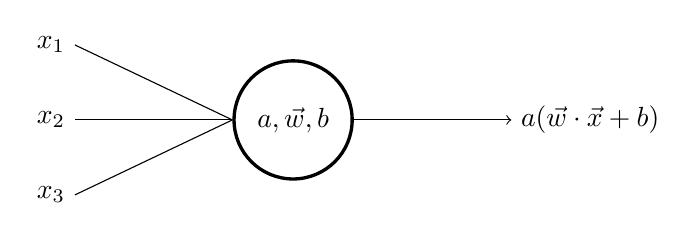
\begin{tikzpicture}[
neuron/.style={circle, draw=black, very thick, minimum size=1.5cm},
dot/.style={circle, draw=black, fill=black, minimum size=0.1cm, inner sep=0pt},
VLineVertex/.style={circle, draw=black, minimum size=0cm, inner sep=0pt},
]

\node[neuron] (neuron) {$a, \vec{w}, b$};
\node (x2) [left=2cm of neuron] {$x_2$};
\node (x1) [above=0.5cm of x2] {$x_1$};
\node (x3) [below=0.5cm of x2] {$x_3$};
\node (out) [right=2cm of neuron] {$a(\vec{w}\cdot\vec{x}+b)$};

\draw (x1.east) -- (neuron.west);
\draw (x2.east) -- (neuron.west);
\draw (x3.east) -- (neuron.west);
\draw [->] (neuron.east) -- (out.west);

\end{tikzpicture}
\caption[Neuron]{Depiction of a neuron with inputs $\vec{x}={(x_1, x_2, x_3)}^T$, weights $\vec{w}$, bias $b$ and activation function $a$.}\label{fig:neuron}
\end{figure}

\medskip
\textcolor{blue}{Use the introduction of the and-neuron from above to introduce the concept of networks in a familiar way. Having logic gates enables us to build more complex structures, such as full adders and hence we can, in principle, calculate any function a computer can calculate. Only afterwards introduce layers as a way of structuring and formalizing networks.}\\
\noindent Since all basic logic gates can be replicated by a neuron, it is a straight forward idea to connect them into more complicated structures, like a full-adder (see \autoref{app:Full_adder}). These structures are than called neural networks, as they are a network of neurons. The example of the full-adder demonstrates the principle of a \gls{nn} perfectly. Its premise is to connect multiple simple functions, the neurons, to form a network, that can solve tasks the individual building blocks can't.\\
In other words, a network aims to calculate some general function by connecting multiple easier functions together. This highlights the importance of the activation function, as it introduces nonlinearities into the network. Without these a neural network would not be able to approximate a nonlinear function such as the XOR-Gate used in \autoref{app:Full_adder} (section 6.1 in \cite{deep_learning_book}), which caused the loss of interest in \gls{nns} around 1940 (section 6.6 in \cite{deep_learning_book}).\medskip\\
Since \gls{nns} are the main subject of \autoref{sec:backpropagation} and since it will be a bit more mathematical, some notation and nomenclature is introduced to structure the networks.\\
Specifically each network can be structured into multiple layers. Each layer consists of one or multiple neurons and each neuron has inputs only from previous layers. Formally we write
\begin{equation}
\mathcal{L}:\R^{k\times l}\times\R^l\times\R^k\to\R^l;\ (W, \vec{b}, \vec{x})\mapsto\mathcal{L}(W,\vec{b},\vec{x})\coloneqq
\begin{pmatrix}
n_1\lr{{(W_1)}^T,b_1,\vec{x}}\\
\vdots\\
n_l\lr{{(W_l)}^T,b_l,\vec{x}}
\end{pmatrix},
\end{equation}
where $n_i$ is neuron $i$ on the layer and $W_i$ is the $i$-th row of a $k\times l$-matrix. In principle this definition can be extended to tensors of arbitrary dimensions. This would however only complicate the upcoming sections notationally and the principle should be clear from this minimal case, as dot products, sums and other operations have their according counterparts in tensor calculus. As a further step of formal simplification we will assume that all neurons $n_i$ share the same activation function $a$. This does not limit the ability of networks that can be written down, since if two neurons have different activation functions, they can be viewed as two different layers connected to the same previous layer. Their output will than be merged afterwards (see \autoref{fig:diff_activation_functions_layer}).\\
\begin{figure}
\centering
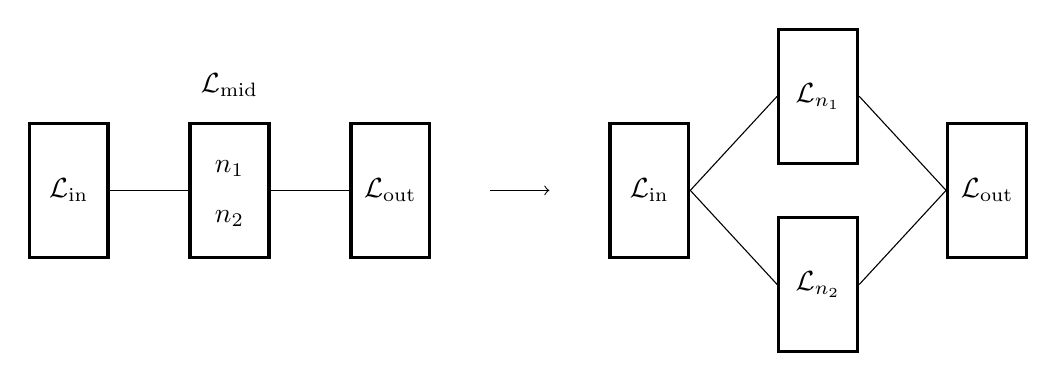
\begin{tikzpicture}[
neuron/.style={circle, draw=black, very thick, minimum size=1.4cm},
dot/.style={circle, draw=black, fill=black, minimum size=0.1cm, inner sep=0pt},
VLineVertex/.style={circle, draw=black, minimum size=0cm, inner sep=0pt},
layer/.style={rectangle, draw=black, very thick, minimum height=1.7cm, minimum width=1cm}
]

\node[layer] (in1) {$\mathcal{L}_\text{in}$};
\node[layer] (n1n2) [right=1cm of in1] {$\oset[4ex]{n_1}{n_2}$};

\node[layer] (out1) [right=1cm of n1n2] {$\mathcal{L}_\text{out}$};
\node (lmid) [above=0.2cm of n1n2] {$\mathcal{L}_\text{mid}$};

\node (arrow_start) [right=0.5cm of out1] {};
\node (arrow_end) [right=0.75cm of arrow_start] {};

\node[layer] (in2) [right=0.5cm of arrow_end] {$\mathcal{L}_\text{in}$};
\node (midpoint) [right=1.5cm of in2] {};
\node[layer] (ln1) [above=0.2cm of midpoint] {$\mathcal{L}_{n_1}$};
\node[layer] (ln2) [below=0.2cm of midpoint] {$\mathcal{L}_{n_2}$};
\node[layer] (out2) [right=1.5cm of midpoint] {$\mathcal{L}_\text{out}$};

%Connections part1
\draw (in1.east) -- (n1n2.west);
\draw (n1n2.east) -- (out1.west);

%Arrow
\draw[->] (arrow_start) -- (arrow_end);

%Connections part2
\draw (in2.east) -- (ln1.west);
\draw (in2.east) -- (ln2.west);
\draw (ln1.east) -- (out2.west);
\draw (ln2.east) -- (out2.west);
\end{tikzpicture}
\caption[Splitting different actvation functions into seperate layers]{Depiction of how a layer ($\mathcal{L}_\text{mid}$) consisting of neurons with different activation functions ($n_1$ and $n_2$) can be split into two separate layers ($\mathcal{L}_{n_1}$ and $\mathcal{L}_{n_2}$).}\label{fig:diff_activation_functions_layer}
\end{figure}

\noindent With this simplification one can write a layer simply as
\begin{equation}
\mathcal{L}(W,\vec{b},\vec{x})=a(W\cdot\vec{x}+\vec{b}),
\end{equation}
where it is understood, that the activation function $a$ acts component wise on the resulting $l$-dimensional vector.\\
In this fashion a network consisting of a chain of layers $\mathcal{L}_\text{in}$, $\mathcal{L}_\text{mid}$, $\mathcal{L}_\text{out}$ can be written as
\begin{align}
\mathcal{N} & \lr{W^\text{in}, \vec{b}^\text{in}, W^\text{mid}, \vec{b}^\text{mid}, W^\text{out}, \vec{b}^\text{out}, \vec{x}}\nonumber\\
\phantom{\mathcal{N}} & \coloneqq\mathcal{L}_\text{out}\lr{W^\text{out}, \vec{b}^\text{out}, \mathcal{L}_\text{mid}\lr{W^\text{mid}, \vec{b}^\text{mid}, \mathcal{L}_\text{in}\lr{W^\text{in}, \vec{b}^\text{in}, \vec{x}}}}\nonumber\\
\phantom{\mathcal{N}} & = a_\text{out}\lr{\vec{b}^\text{out}+W^\text{out}\cdot a^\text{mid}\lr{\vec{b}^\text{mid}+W_\text{mid}\cdot a_\text{in}\lr{\vec{b}^\text{in}+W_\text{in}\cdot \vec{x}}}}.
\end{align}
Hence a network can be understood as a set of nested functions.\\
An important point with the definitions above is that the layers get their input only from their preceding layers. Especially no loops are allowed, i.e. getting input from some subsequent layer is not permitted. A network of the first kind is called a \emph{feed forward neural network} (\gls{ffn}), as the input to the network is propagated from front to back, layer by layer and each layer gets invoked only once. There are also other architectures called \emph{recurrent neural networks} (\gls{rnn}), which allow for loops and work by propagating the activations in discrete time steps. These kinds of networks are in principle closer to the inner workings of the human brain, but in practice show worst performance and are therefore not used or discussed further in this work. \textcolor{red}{[Citations], maybe also mention that RNNs have shown good performance in time series data (which we are working with) but other studies (paper Frank sent around) have shown that TCN also do the job}\\
A \gls{ffn} can in general be grouped into three different parts called the input-, output- and hidden layer/layers. The role of the input- and output-layers is self explanatory; they are the layers where data is fed into the network or where data is read out. Therefore their shape is determined by the data the network is being fed and the expected return. The hidden-layers on the contrary are called ''hidden'', as their shape and size is not defined by the data. Furthermore the hidden layers do not see the input or labels directly, which means that the network itself has to ''decide'' on how to use them (page 165 in \cite{deep_learning_book}). \autoref{fig:hidden_layer} shows an example of a simple network with a single hidden layer. In principle there could be any number of hidden layers with different sizes. In this example the input is n-dimensional and the output 2-dimensional. If the input was changed to be (n-1)-dimensional, the same hidden-layer could be used, as its size does not depend on the data or output. Therefore, when designing a network architecture, one designs the shape and functionality of the hidden layers. How well it performs is mainly governed by theses layers. Two networks with different hidden layers are also called different architectures. The architecture of a neural network hence describes how all layers of the network behave and are connected. \textcolor{red}{[Can I find citation for these last statements?]}\\
A \gls{nn} is called \emph{deep}, if it has multiple hidden layers. The depth of a network analogously is number of layers at the longest path to an output layer. \textcolor{red}{[Citation]}
\begin{figure}
\centering
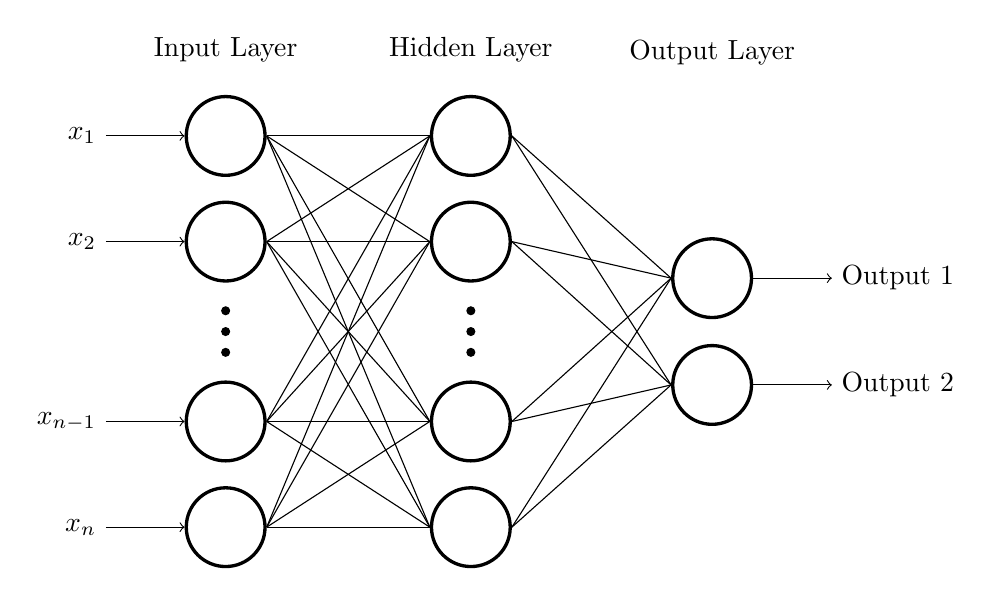
\begin{tikzpicture}[
neuron/.style={circle, draw=black, very thick, minimum size=1cm, transform shape},
dot/.style={circle, draw=black, fill=black, minimum size=0.1cm, inner sep=0pt, transform shape},
note/.style={circle, draw=black, minimum size=0pt, inner sep=0pt, transform shape},
]

%Input Layer neurons
\node[neuron] (inp_1) {};
\node[neuron] (inp_2) [below=0.3cm of inp_1] {};
\node[dot] (inp_v_1) [below=0.3cm of inp_2] {};
\node[dot] (inp_v_2) [below=0.15cm of inp_v_1] {};
\node[dot] (inp_v_3) [below=0.15cm of inp_v_2] {};
\node[neuron] (inp_3) [below=0.3cm of inp_v_3] {};
\node[neuron] (inp_4) [below=0.3cm of inp_3] {};
\node (inp_label) [above=0.3cm of inp_1] {Input Layer};

%Hidden Layer neurons
\node[dot] (hid_v_2) [right=3cm of inp_v_2] {};
\node[dot] (hid_v_1) [above=0.15cm of hid_v_2] {};
\node[dot] (hid_v_3) [below=0.15cm of hid_v_2] {};
\node[neuron] (hid_2) [above=0.3cm of hid_v_1] {};
\node[neuron] (hid_1) [above=0.3cm of hid_2] {};
\node (hid_label) [above=0.3cm of hid_1] {Hidden Layer};
\node[neuron] (hid_3) [below=0.3cm of hid_v_3] {};
\node[neuron] (hid_4) [below=0.3cm of hid_3] {};

%Output Layer neurons
\node[note] (out_mid) [right=3cm of hid_v_2] {};
\node[neuron] (out_1) [above=0.15cm of out_mid] {};
\node[neuron] (out_2) [below=0.15cm of out_mid] {};
\node (out_label) [above=3.25cm of out_mid] {Output Layer};

%Inputs
\node (x1) [left=1cm of inp_1] {$x_1$};
\node (x2) [left=1cm of inp_2] {$x_2$};
\node (x3) [left=1cm of inp_3] {$x_{n-1}$};
\node (x4) [left=1cm of inp_4] {$x_n$};

%Outputs
\node (o1) [right=1cm of out_1] {Output 1};
\node (o2) [right=1cm of out_2] {Output 2};

%Connections Input Layer - Hidden Layer
\draw (inp_1.east) -- (hid_1.west);
\draw (inp_1.east) -- (hid_2.west);
\draw (inp_1.east) -- (hid_3.west);
\draw (inp_1.east) -- (hid_4.west);

\draw (inp_2.east) -- (hid_1.west);
\draw (inp_2.east) -- (hid_2.west);
\draw (inp_2.east) -- (hid_3.west);
\draw (inp_2.east) -- (hid_4.west);

\draw (inp_3.east) -- (hid_1.west);
\draw (inp_3.east) -- (hid_2.west);
\draw (inp_3.east) -- (hid_3.west);
\draw (inp_3.east) -- (hid_4.west);

\draw (inp_4.east) -- (hid_1.west);
\draw (inp_4.east) -- (hid_2.west);
\draw (inp_4.east) -- (hid_3.west);
\draw (inp_4.east) -- (hid_4.west);

%Connections Hidden Layer - Output Layer
\draw (hid_1.east) -- (out_1.west);
\draw (hid_1.east) -- (out_2.west);

\draw (hid_2.east) -- (out_1.west);
\draw (hid_2.east) -- (out_2.west);

\draw (hid_3.east) -- (out_1.west);
\draw (hid_3.east) -- (out_2.west);

\draw (hid_4.east) -- (out_1.west);
\draw (hid_4.east) -- (out_2.west);

\draw[->] (x1) -- (inp_1.west);
\draw[->] (x2) -- (inp_2.west);
\draw[->] (x3) -- (inp_3.west);
\draw[->] (x4) -- (inp_4.west);

\draw[->] (out_1.east) -- (o1);
\draw[->] (out_2.east) -- (o2);
\end{tikzpicture}
\caption[Simple neural network]{A depiction of a simple network with a single input-, hidden- and output-layer. The input-data is a n-dimensional vector ${(x_1, \dotsc, x_n)}^T$ and the output is a 2-dimensional vector. In this picture it looks like the hidden layer has the same number of neurons as the input layer. This does not necessarily have to be the case. Lines between two neurons indicate, that the output of the left neuron serves as weighted input for the right one.}\label{fig:hidden_layer}
\end{figure}

\subsection{Backpropagation}\label{sec:backpropagation}
\textcolor{red}{The beginning of this section feels very wordy and repetitive. Break it down!}\\
In \autoref{sec:basics_neuron_network} the basics of a \gls{nn} where discussed and the example of a network replicating a binary full-adder showed the potential of these networks, when the weights and biases are chosen correctly. The example actually proofs that a sufficiently complicated network can - in principle - calculate any function a computer can, as a computer is just a combination of logic gates, especially binary full-adders.\footnote{There is an even stronger statement called the universal approximation theorem, which states that any Borel measurable function on a finite-dimensional space can be approximated to any degree with a \gls{nn} with at least one single hidden layer of sufficient size. (p. 194 \cite{deep_learning_book})}\cite{deep_learning_beginning}\\
The question therefore is how to choose the weights in a network for it to approximate some function optimally. For the binary full-adder the weights and biases were chosen by hand, as the problem the network was trying to solve was rather simple. A more general approach however would be beneficial, as not all problems are this simple. Therefore the goal is to design some network and let it learn/optimize the weights and biases such that the error between the actual function and the estimate of the network is minimal.\\
To do this, some known and labeled data is necessary, in order for the network being able to compare its output to some ground truth and adjust its weights and biases to minimize some error function. This way of optimizing the weights and biases is called \emph{training}. The data used during training is hence called training data or training set. To be a bit more specific, the analyzed data in this work is some time series. The output of this analysis will be some scalar number; the \gls{snr}. Therefore the network receives some data as input, of which the true \gls{snr}-value is known. This true value will be called \emph{label}\footnote{For regression problems this value is often also called target value. We will however stick to calling it the label for our training data.} from here on out. The network will produce some value from this input data and compare it to what \gls{snr} was provided as label. From there it will try to optimize the weights and biases to best fit the function that maps $\text{data}\to\text{\gls{snr}}$. This process of optimizing the weights and biases in the way described below is enabled by a process called backpropagation, as the error propagates from the last to the first layer. The meaning of this will become clearer in the upcoming paragraphs.\\
So far only the abstract term ''error'' was used. This error, in machine learning language, is called the \emph{loss function} and in general is defined by
\begin{equation}\label{def:general_loss}
L:\R^{l\times k}\times\R^{l\times k}\to\R;\ (y_\text{net}, y_\text{label})\mapsto L(y_\text{net}, y_\text{label}),
\end{equation}
where $l$ is the number of training samples used to estimate the error and $k$ is the dimension of the network output.\\
When doing a regressive fit, one of the standard error functions is the \emph{mean squared error} (\gls{mse}), which is the loss function mainly used in this work and that is defined by
\begin{equation}\label{def:loss_mean_squared_error}
L:\R^{l\times k}\times\R^{l\times k}\to\R;\ (y_\text{net}, y_\text{label})\mapsto L(y_\text{net}, y_\text{label})\coloneqq\frac{1}{l}\sum_{i=1}^l{(\vec{y}_{\text{net},i}-\vec{y}_{\text{label},i})}^2.
\end{equation}
A more thorough discussion and justification for using \gls{mse} as loss can be found in section 5.5 and 6.2.1.1 of \cite{deep_learning_book}.\\
To minimize this loss, the weights and biases of the different layers are changed, usually using an algorithm called \emph{gradient decent}. It works by calculating the gradient of some layer with respect to its weights and biases and taking a step in the opposite direction. For notational simplicity we'll denote the weights and biases of a network by $\theta$ and call them collectively parameters. It is understood that $\theta=\lr{W^{1},b^1, W^2, b^2, \cdots}$. Gradient decent is than given by
\begin{equation}\label{def:gradient_decent}
\theta '=\theta - \epsilon\ \nabla_\theta L\lr{y_\text{net}(\theta), y_\text{label}},
\end{equation}
where $\epsilon$ is called learning rate and controls how large of a step is taken on each iteration.\\
This formula assumes, that all samples from the training set are used to calculate the gradient. In practice this would be too computationally costly. Therefore the training set is split into multiple parts, called mini-batches. A step of the gradient decent is than made using only the samples from one mini-batch. This alteration of gradient decent goes by the name of \emph{stochastic gradient decent} (\gls{sgd}). The larger the mini-batch, the more accurate the estimate of the gradient and therefore the fewer steps are needed to get to lower values of the loss. Each step however takes longer to calculate. This means one has to balance the benefits and drawbacks of the mini-batch size.\medskip\\
The real work of training a network now lies in calculating the gradient $\nabla_\theta L\lr{y_\text{net}(\theta), y_\text{label}}$, which is a challenge, as $\theta$ usually consists of at least a few hundred thousand weights and biases. The algorithm, that is used to calculate this gradient, is called backpropagation or simply backprop and is mostly a iterative application of the chain rule.\\
For simplicity assume we have a network $\mathcal{N}\lr{\theta, \vec{x}}$ consisting of $n$ consecutive layers $\mathcal{L}^1,\cdots,\mathcal{L}^n$ with weights $W^1,\cdots,W^n$, biases $\vec{b}^1,\cdots,\vec{b}^n$ and activation functions $a_1,\cdots, a_n$. The network will be trained by minimizing the loss given in \eqref{def:loss_mean_squared_error}. Calculating the gradient $\nabla_\theta L\lr{y_\text{net}(\theta), y_\text{label}}$ requires to calculate $\nabla_{W^1}L, \cdots,\nabla_{W^n}L$ and $\nabla_{\vec{b}^1}L,\cdots,\nabla_{\vec{b}^n}L$, where
\begin{equation}\label{def:matrix_gradient}
\nabla_{W^i}L\coloneqq
\begin{pmatrix}
	\partial_{W^i_{11}}L & \cdots & \partial_{W^i_{1l}}L\\
	\vdots & \ddots & \vdots\\
	\partial_{W^i_{k1}}L & \cdots & \partial_{W^i_{kl}}L
\end{pmatrix},
\end{equation}
for $W^i\in \R^{k\times l}$ and
\begin{equation}\label{def:vector_gradient}
\nabla_{\vec{b}^i}L\coloneqq
\begin{pmatrix}
	\partial_{b^i_1}L\\
	\vdots\\
	\partial_{b^i_k}L
\end{pmatrix},
\end{equation}
for $\vec{b}^i\in\R^k$.\\
To calculate $\partial_{W^i_{jk}}L$ and $\partial_{b^i_j}L$, define
\begin{align}\label{def:backprop_z}
z^n & \coloneqq\vec{b}^n+W^n\cdot a_{n-1}\lr{z^{n-1}}\nonumber\\
z^1 & \coloneqq\vec{b}^1+W^1\cdot\vec{x},
\end{align}
such that
\begin{equation}
\mathcal{N}\lr{\theta,\vec{x}}=a_n\lr{z_n}.
\end{equation}
To save another index, we will assume a mini-batch size of 1. For a larger mini-batch size one simply has to average over the individual gradients, as sums and derivatives commute.\\
With this in mind, the loss is given by
\begin{equation}
L\lr{y_\text{net}, y_\text{label}}=L\lr{\mathcal{N}\lr{\theta,\vec{x}}, y_\text{label}}=L\lr{a_n\lr{z_n}, y_\text{label}}=\lr{a_n\lr{z_n}- \vec{y}_\text{label}}^2.
\end{equation}
To start off derive this loss by the parameter $\theta_j$
\begin{equation}
\partial_{\theta_j}\lr{a_n\lr{z_n}- \vec{y}_\text{label}}^2=\lr{\partial_{\theta_j}a_n\lr{z_n}}\lr{2\lr{a_n\lr{z_n}- \vec{y}_\text{label}}}
\end{equation}
From there calculate $\partial_{\theta_j}a_n\lr{z_n}$, remembering, that $a_n$ and $z_n$ are both vectors.
\begin{align}\label{def:start_backprop}
\partial_{\theta_j}a_n\lr{z_n} & = \partial_{\theta_j}\sum_i a_n^i\lr{z_{n,1}\lr{\theta_j},\dotsc, z_{n,k}\lr{\theta_j}} \vec{e}_i\nonumber\\
& = \sum_i \sum_{m=1}^k \lr{\partial_{\theta_j}z_{n, m}\lr{\theta_j}}\lr{\partial_{z_{n, m}} a_n^i\lr{z_{n,1}\lr{\theta_j},\dotsc, z_{n,k}\lr{\theta_j}}} \vec{e}_i\nonumber\\
& = \sum_i \lr{\lr{\partial_{\theta_j}z_n}\cdot \lr{\nabla_{z_n} a_n^i}}\vec{e}_i
\end{align}
Since all activation functions $a_n^i$ on a layer are the same, the gradient $\lr{\nabla_{z_n} a_n^i}$ simplifies to $\partial_z \restr{a(z)}{z=z_{n,i}}$. With this one gets
\begin{equation}\label{def:start_backprop_simple}
\partial_{\theta_j}a_n\lr{z_n} = \lr{\partial_{\theta_j} z_n} \odot \partial_z \restr{a_n(z)}{z=z_n},
\end{equation}
where $\odot$ denotes the Hadamard product.
The final step to understanding backpropagation is to evaluate $\partial_{\theta_j}z_n$. For now assume that $\theta_j$ is some weight on a layer that is not the last layer.
\begin{align}\label{def:backprop_recurs_1}
\partial_{\theta_j}z_n & = \partial_{\theta_j}\lr{\vec{b}^n+W^n\cdot a_{n-1}\lr{z_{n-1}}}\nonumber\\
& = \partial_{\theta_j}\lr{W^n\cdot a_{n-1}\lr{z_{n-1}}}\nonumber\\
& = W^n\cdot\partial_{\theta_j}a_{n-1}\lr{z_{n-1}}
\end{align}
Inserting \eqref{def:backprop_recurs_1} into \eqref{def:start_backprop_simple} yields the recursive relation
\begin{equation}\label{def:backprop_recursive_relation}
\partial_{\theta_j}a_n\lr{z_n} = \lr{W^n\cdot\partial_{\theta_j}a_{n-1}\lr{z_{n-1}}}\odot\partial_z \restr{a_n(z)}{z=z_n}.
\end{equation}
The recursion stops, when it reaches the layer the weight $\theta_j$ is located on and evaluates to (assuming $\theta_j$ is part of layer $k$)
\begin{equation}\label{def:recursion_stop_weight}
\partial_{\theta_j}a_k\lr{z_k}=\lr{\partial_{\theta_j}W^k}\cdot a_{k-1}\lr{z_{k-1}}.
\end{equation}
The derivative can also be expressed in an analytical form, by utilizing, that the Hadamard product is commutative and can be expressed in terms of matrix multiplications. To do so define
\begin{equation}
\left[\Sigma\lr{\vec{x}}\right]_{ij}=
\begin{cases}
	x_i,& i = j\\
	0,& \text{otherwise}
\end{cases}.
\end{equation}
With this definition equation \eqref{def:backprop_recursive_relation} can be written as
\begin{equation}
\partial_{\theta_j}a_n\lr{z_n} = \Sigma\lr{\partial_z \restr{a_n(z)}{z=z_n}}\cdot W^n\cdot\partial_{\theta_j}a_{n-1}\lr{z_{n-1}}
\end{equation}
and the recursion can be solved to yield
\begin{equation}\label{def:backprop_analytical_weight}
\partial_{\theta_j}a_n\lr{z_n} = \left[\prod_{l=0}^{n-k+1}\Sigma\lr{\restr{\partial_z a_{n-l}\lr{z}}{z=z_{n-l}}}\cdot W^{n-l}\right]\cdot \Sigma\lr{\restr{\partial_z a_k\lr{z}}{z=z_k}}\cdot\lr{\partial_{\theta_j}W^k}a_{k-1}\lr{z_{k-1}}.
\end{equation}
\textcolor{red}{If there is time, check the equations below, as I did not thoroughly recompute them.}\\
The same computation can be done if $\theta_j$ is a bias instead of a weight. When this computation is done, equation \eqref{def:backprop_recursive_relation} still holds, but the stopping condition \eqref{def:recursion_stop_weight} is simplified to
\begin{equation}
\partial_{\theta_j}a_k\lr{z_k}=\partial_{\theta_j}\vec{b}^k.
\end{equation}
From this the analytic form can be computed to be
\begin{equation}\label{def:backprop_analytical_bias}
\partial_{\theta_j}a_n\lr{z_n} = \left[\prod_{l=0}^{n-k+1}\Sigma\lr{\restr{\partial_z a_{n-l}\lr{z}}{z=z_{n-l}}}\cdot W^{n-l}\right]\cdot \Sigma\lr{\restr{\partial_z a_k\lr{z}}{z=z_k}}\cdot\partial_{\theta_j}\vec{b}^k.
\end{equation}
The recursive formula \eqref{def:backprop_recursive_relation} now justifies the term ''backpropagation''. When a sample is evaluated, it is passed from layer to layer starting at the front. Therefore this is called a \emph{forward pass}. The output the network gives for a single forward pass will probably differ from the label and hence has an error (quantified by the loss function). This error is used to calculate the gradient and adjusts the parameters of the network. The way this is done is given by \eqref{def:backprop_recursive_relation}. It starts at the last layer and propagates back through the network until it reaches the layer of the weight that should be adjusted.\\
With these formulae one could in principle calculate the gradient of the loss with respect to all parameters $\theta$ and use this gradient to optimize and train a network. In reality this would still be too slow and computationally costly. Instead each layer (or rather each operation) has a backpropagation method associated to it, that returns the gradient based on a derivative to one of its inputs and the gradient from the previous layer.\\
For clarification, consider an operation that multiplies two matrices $A$ and $B$ and say the gradient calculated by the backpropagation method of the previous layer returned $G$ as its gradient. The backpropagation method for the matrix multiplication now needs to implement the derivative with respect to $A$ and the derivative with respect to $B$. Thus it will return $G\cdot B^T$ when derived by $A$ and $G\cdot A^T$ when derived by $B$. (section 6.5.6 \cite{deep_learning_book})\\
The full backpropagation algorithm than only has to call the backpropagation methods of each layer/operation. (For a more thorough discussion see section 6.5 of \cite{deep_learning_book}.)

\subsection{Training and Terminology}\label{sec:training}
In the previous \autoref{sec:backpropagation} the backpropagation algorithm was introduced as the method used for the network to learn. It used some labeled data to compare its output to and adjust the parameters accordingly. This labeled data was called the training set. In principle the network could be trained over and over again on the same data to further improve the performance of the network. This is done to some extend in practice. An entire pass of the training set is called an \emph{epoch}. In theory, the worst one could fear for is a gradient that vanishes, as the global or a local minimum in the loss is reached.\\
In practice this is true only partially. At some point the network will start ''memorizing'' the samples it has seen in the training set. When a network shows this behavior during training it is called \emph{overfitting}. This is a problem not only known in machine learning but also with regressive fits and has the same reason; too many free parameters. Consider a parabola sampled at $n$ points. If a regressive fit is done, the best choice for the model would be a parabola $f(x)=a x^2+b x + c$ with the three free parameters $a$, $b$ and $c$. If $n\geq 3$ a regressive fit minimizing the \gls{mse} would recover the original parabola that was sampled by the $n$ points. However one could also use a polynomial of degree $m\geq n$ as a model to find a function that runs exactly through all $n$ points and thus minimizes the \gls{mse} to the same value of zero too. (see \autoref{fig:overfitting})\\
There are however two differences between the two cases. The most obvious one is the number of free parameters. The parabola has three parameters, whereas the polynomial of degree $m$ has $m+1$ free parameters. As $m\geq n$ was required, there is at least one parameter that cannot be fixed by the data and is therefore still free. The second difference is the behavior of the \gls{mse} when the fitted model is evaluated on a point, that is not part of the set of points, that was used to generate the fit. For the parabola the \gls{mse} will stay zero, for the polynomial of degree $m$ however the \gls{mse} will most likely be greater than zero, as the true parabola isn't matched. (Compare lower right of \autoref{fig:overfitting}) The first difference explains why overfitting takes place, there are too many parameters that can be varied, the second difference gives a way to detect when overfitting takes place. If the \gls{mse} rises on samples that were not used for the regression, overfitting takes place.\\
The same concept can than be applied to \gls{nns}; if the loss of a network is bigger on different data than that used during training, the network is said to overfit. This second set of samples is called the validation set, as it validates the training. Obviously the data in the validation set must stem from the same underlying procedure, that generated the training set. In the context of this work this means, that the waveforms of the training and validation set must share the same parameter-space.\\
Contrary to overfitting, there is also a phenomenon called \emph{underfitting}. This occurs, when the number of free, i.e. trainable, parameters of a network is too low. It manifests usually in an occasionally lower loss value of the validation set when compared to the training set. To overcome this issue one can simply increase the number of trainable parameters the network has. Increasing the number of trainable parameters is also called increasing the \emph{capacity} of the network.\\
Though underfitting is possible, overfitting is usually a lot more common. There are multiple ways to deal with a network, that overfits during training. The first one would be to reduce the capacity of the network. If that is not possible or worsens the results, the second most easy way is to increase the number of samples in the training set. In the realm of this work, this is a possibility, as we use simulated data, that can be generated on demand. For a lot of other applications however this is not feasible and other means are necessary. One way is to use a technique called regularization, which is explained in \autoref{sec:regularization} and applied to our networks as well. Another one, which will not be discussed in detail here, is data augmentation\footnote{Data augmentation is the process of applying transformations to the input samples, to artificially create more data. The transformation have to act in such a way that the resulting data is similar in its properties to the original data.}. (See section 7.4 of \cite{deep_learning_book})\\
To tune out the generalization error, which is the loss value of the validation set, one adjusts the architecture. If there are multiple different architectures, the best one is chosen by the performance on the validation set. In this way, the validation set is also used to fit the model, as in the end the human who trains the models selects the best performing network. Therefore all given results, that did not occur during training\footnote{An example of a result that comes from training the network would be the loss history.}, come from a third independent set. This set is than called the test set.\medskip\\
A general approach to increase the performance of a network is to increase its depth. This is due to two reasons. First of all it has been shown, that a deep network can separate the underlying function it is trying to learn into piecewise linear regions. The number of these regions is than exponential in the depth of the network. Secondly each layer can be viewed as a filter, that looks for certain features in the data. Having multiple stacked layers will enable the network to learn low level features on early layers and combine them into more difficult features on lower layers. (Section 6.4.1 \cite{deep_learning_book}) This idea will be expanded upon in the following \autoref{sec:cnn}. The depth is not the only parameter of a simple network, that can be scaled to increase performance. A systematic study can be found for instance in \cite{efficient_net}.\\
A common problem, that arises when training very deep \gls{nns} is the vanishing gradient problem; the gradient calculated by \eqref{def:backprop_analytical_weight} or \eqref{def:backprop_analytical_bias} is close to zero on early layers, which results in these layers not changing their weights enough. The reason for this behavior can also be understood from \eqref{def:backprop_analytical_weight} and \eqref{def:backprop_analytical_bias}. If the products satisfy $\left|\partial_z a_i(z)\cdot W^i\right|<1$ the gradient is exponentially diminished by the depth of the network.\\
The opposite can also happen. If $\left|\partial_z a_i(z)\cdot W^i\right|>1$ for most of the layers, the gradient will grow exponentially. This behavior is therefore called the exploding gradient problem. (Chapter 5 \cite{deep_learning_beginning})\\
To overcome these problems, one can simply train for longer periods in the case of the vanishing gradient problem (Chapter 5 \cite{deep_learning_beginning}), use multiple points at which the loss is calculated \cite{inception_module} or adjust the initialization of the weights. Another solution introduced by \cite{residual_connections_invention} are residual connections. These are connections of a layers input to its output. Specifically, the input of the layer is added back onto its output. The idea behind this connection is to make it easier for the network to learn an identity mapping by simply setting the weights of the layer to zero. This showed great improvements and the ability to have very deep networks\cite{residual_connections_invention}.
\begin{figure}
\centering
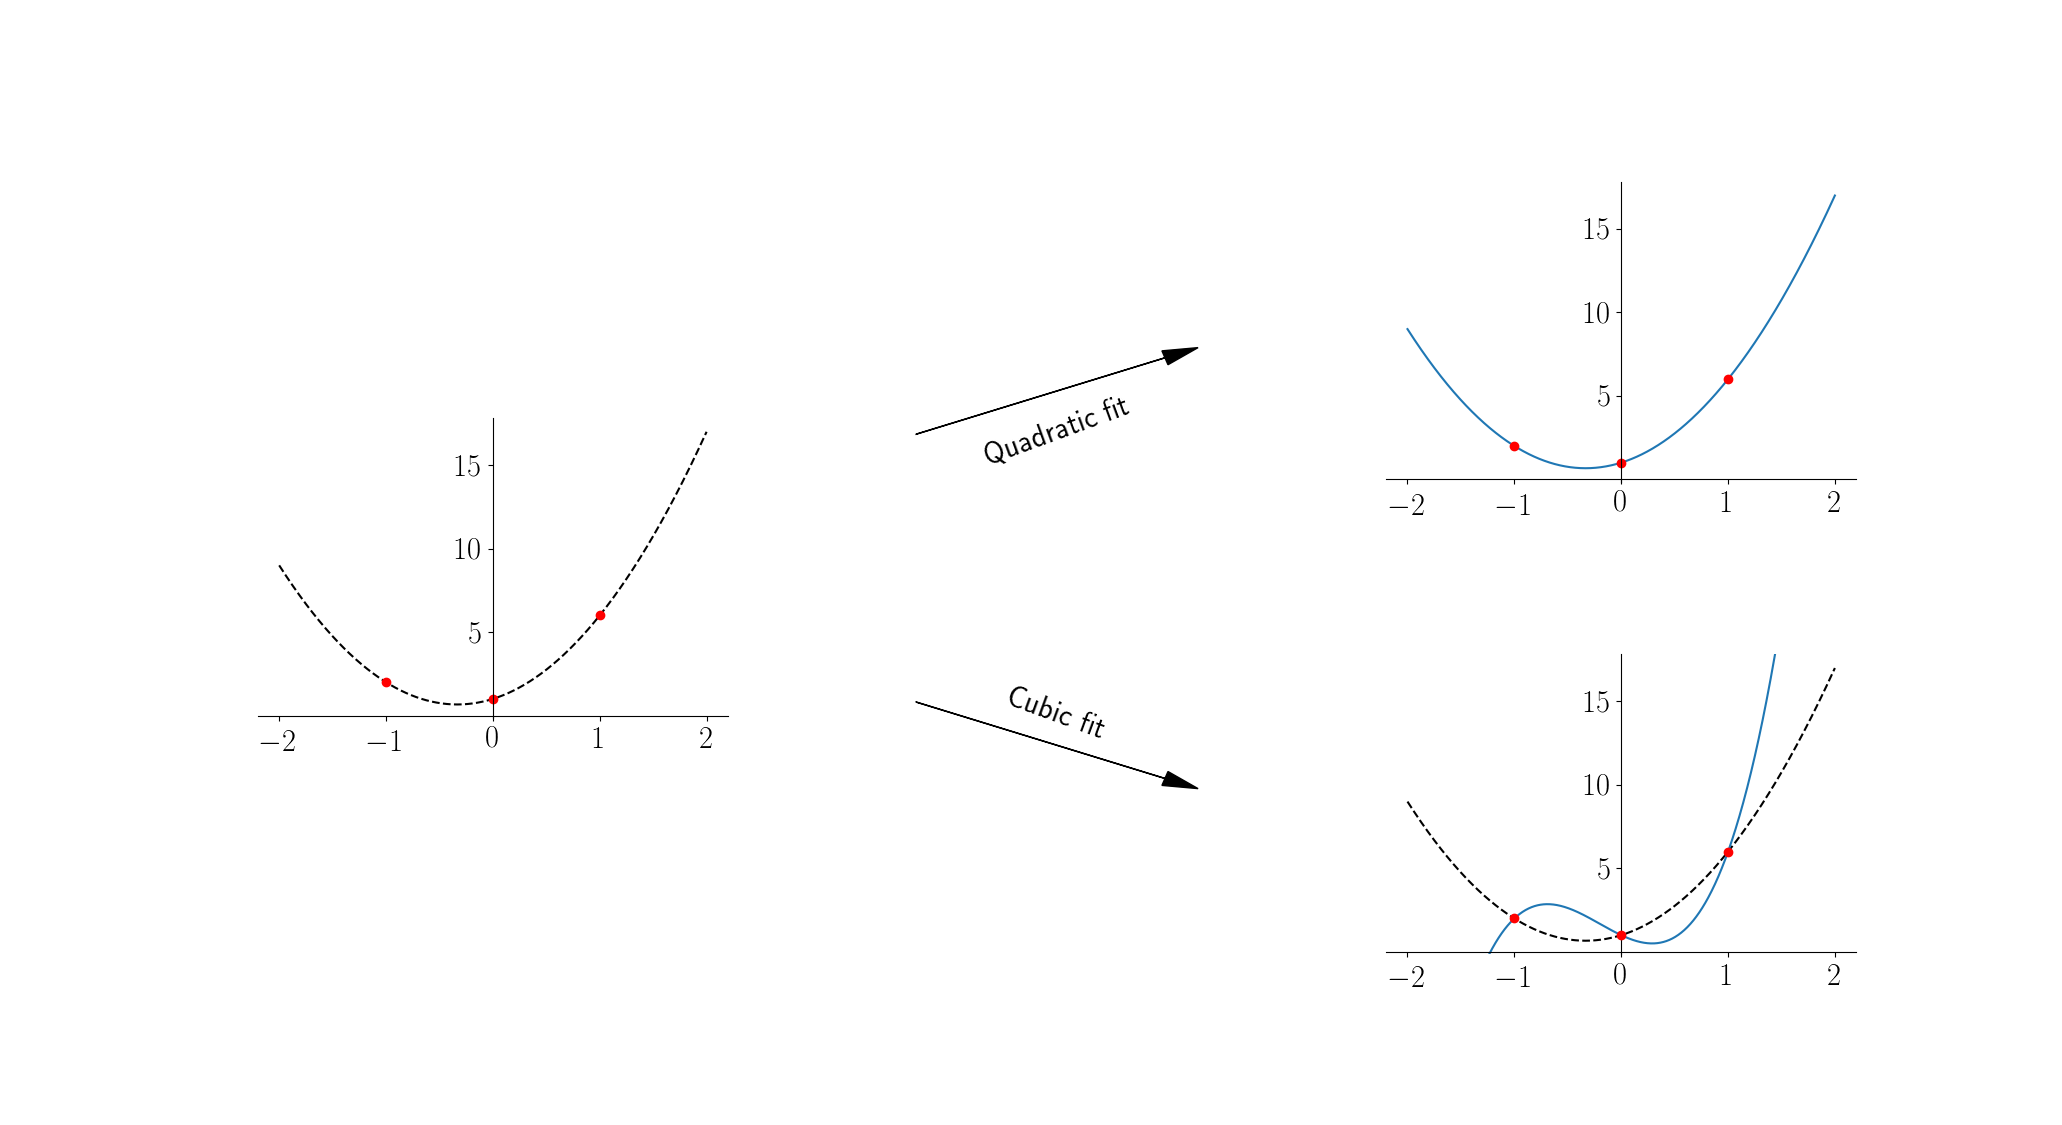
\includegraphics[width=\textwidth]{overfitting.png}
\caption[Overfitting]{Depiction of overfitting in the classical regression. On the left the originally sampled function $f(x)\coloneqq 3x^2 + 2x + 1$ is shown in dashed and black. The red dots are the samples that are being used for the regression on the right. The top right shows the regression, where $g(x)=a x^2 + b x + c$ was used as a basis and recovered the correct parameters $a=3$, $b=2$ and $c=1$. All free parameters are fixed by the data. The lower right plot shows a case of overfitting. The same three points are now used to fit the four free parameters $a$, $b$, $c$ and $d$ of the function $h(x)=a x^3 + b x^2 + c x + d$. The analytic solution returns $b=3$, $c=2-a$ and $d=1$ with $a$ being free. Therefore a possible regression could use $a=5$, which is used in the lower right plot. The points used for regression are all hit, hence the \gls{mse} is zero. However if another point on the black dashed line would be used, the fitted model would be off and the \gls{mse} would be non-zero.}\label{fig:overfitting}
\end{figure}

\subsection{Convolution Neural Networks}\label{sec:cnn}
In the previous sections only fully connected layers were used to build networks. These are layers, where each neuron is connected to every neuron on the previous layer. (See \autoref{fig:dense_layer}) These fully connected layers are called \emph{dense} layers. In this section a different kind of layer and variants of it will be motivated and introduced. It is the main driving force of modern neural networks and is called convolution layer.
\begin{figure}
\centering
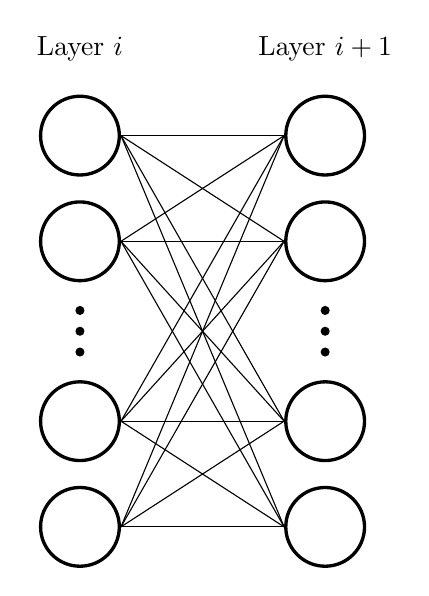
\begin{tikzpicture}[
neuron/.style={circle, draw=black, very thick, minimum size=1cm, transform shape},
dot/.style={circle, draw=black, fill=black, minimum size=0.1cm, inner sep=0pt, transform shape},
note/.style={circle, draw=black, minimum size=0pt, inner sep=0pt, transform shape},
]

%Input Layer neurons
\node[neuron] (inp_1) {};
\node[neuron] (inp_2) [below=0.3cm of inp_1] {};
\node[dot] (inp_v_1) [below=0.3cm of inp_2] {};
\node[dot] (inp_v_2) [below=0.15cm of inp_v_1] {};
\node[dot] (inp_v_3) [below=0.15cm of inp_v_2] {};
\node[neuron] (inp_3) [below=0.3cm of inp_v_3] {};
\node[neuron] (inp_4) [below=0.3cm of inp_3] {};
\node (inp_label) [above=0.3cm of inp_1] {Layer $i$};

%Hidden Layer neurons
\node[dot] (hid_v_2) [right=3cm of inp_v_2] {};
\node[dot] (hid_v_1) [above=0.15cm of hid_v_2] {};
\node[dot] (hid_v_3) [below=0.15cm of hid_v_2] {};
\node[neuron] (hid_2) [above=0.3cm of hid_v_1] {};
\node[neuron] (hid_1) [above=0.3cm of hid_2] {};
\node (hid_label) [above=0.3cm of hid_1] {Layer $i+1$};
\node[neuron] (hid_3) [below=0.3cm of hid_v_3] {};
\node[neuron] (hid_4) [below=0.3cm of hid_3] {};

%Connections Input Layer - Hidden Layer
\draw (inp_1.east) -- (hid_1.west);
\draw (inp_1.east) -- (hid_2.west);
\draw (inp_1.east) -- (hid_3.west);
\draw (inp_1.east) -- (hid_4.west);

\draw (inp_2.east) -- (hid_1.west);
\draw (inp_2.east) -- (hid_2.west);
\draw (inp_2.east) -- (hid_3.west);
\draw (inp_2.east) -- (hid_4.west);

\draw (inp_3.east) -- (hid_1.west);
\draw (inp_3.east) -- (hid_2.west);
\draw (inp_3.east) -- (hid_3.west);
\draw (inp_3.east) -- (hid_4.west);

\draw (inp_4.east) -- (hid_1.west);
\draw (inp_4.east) -- (hid_2.west);
\draw (inp_4.east) -- (hid_3.west);
\draw (inp_4.east) -- (hid_4.west);
\end{tikzpicture}
\caption[Dense layer]{\textcolor{red}{Insert description! Maybe inprove this graphic.}}\label{fig:dense_layer}
\end{figure}

\subsubsection{Convolution Layer}\label{sec:convolution_layer}
\textcolor{blue}{What are the advantages of convolution layers and why do we use them? Disadvantages?}
Dense layers have been the starting point for deep \gls{nns} and are used to derive a lot of the theory. In \autoref{sec:training} it was stated, that deeper networks usually perform better. This is however a problem for \gls{nns} that consist only of dense layers, as the number of trainable parameters grows exponentially \textcolor{red}{[Citation, can't find one]}, if the layer size is kept constant between two layers. This causes computational limits that limit the depth.\\
Another problem of fully connected layers is that they are rather static. Being static means, that it is hard for the network to adapt to slight changes in the data. To understand this, consider a network that learns to distinguish between cats and dogs. Say, that for the training set all animals are in the lower left hand corner of the image. The validation set than might have the animals not in the lower left, but the upper right corner. A \gls{nn} consisting purely of dense layers might not be able to adapt to this new position. Even if there are animals in the top right corner for the training set, the network might need a lot of layers and trainable parameters to learn all possible positions.\\
These restrictions led to the invention of the convolution layer in 1989. \cite{convolution_layer_invention} Though it was originally conceived in its 2 dimensional variant, only the 1 dimensional convolution layer will be explained here.\footnote{The core concepts are the same, thus the concept can easily be adapted to any number of dimensions.} Contrary to dense layers, the neurons of convolution layers are only connected to a few neurons on the previous layer. Furthermore these connections all share the same weight. Thus one can view a convolution layer as a filter of learnable weights that slide across the input, in a way convolving the the filter with the input data. (see \autoref{fig:simple_convolution})\\
The size of the filter, i.e. how many entries it spans, is called the \emph{kernel size}. If multiple convolution layers with the same kernel size are stacked, the number of trainable parameters increases only linearly with the depth, which is a huge improvement over dense layers.\\
The capacity of a convolution layer however is not only governed by the kernel size, but also by how many filters are run over the same data in parallel. If a convolution layer runs only a single filter over the data, it might learn to detect a single feature, like a vertical line. Therefore multiple filters, that have different weights, are usually run over the same input data. Each of these different filters will than be able to detect different features. The output these layers produce are called \emph{feature maps}.\\
Having multiple filters however changes the shape of the output from being 1 dimensional, with just a single filter, to being 2 dimensional with multiple filters. The data each filter outputs is still 1 dimensional and called a \emph{channel} of the final output. To be able to stack convolution layers, they take in a 2 dimensional input and are specified by the number of filters and the kernel size of all these filters\footnote{Usually all filters have the same kernel size.}. Each filter, that is convolved with the data, spans all channels. The kernel size only specifies how many entries in each channel are used. (see \autoref{fig:convolution_channels}) \textcolor{red}{This paragraph is hard to read and understand.}\\
As an example say we specify a convolution layer by having $32$ filters and a kernel size of $3$. Now we use this convolution layer on two different inputs. Input 1 has a shape of $4096\times 1$ and input 2 has a shape of $4096\times 2$. Notice, that input 1 in principle is still 1 dimensional, as it only has one channel. The data still has to be reshaped though to work with the general concept. For input 1, the filter would be of shape $3\times 1$ and the output shape of the convolution layer would be $4094\times 32$. Therefore the convolution layer would have $3\cdot 1\cdot 32=96$ trainable parameters. For input 2, the filter would need to span both channels and thus has the shape $3\times 2$, the output shape however is still $4094\times 32$. The number of trainable parameters however also doubles to $3\cdot 2\cdot 32=192$. All of the above disregarded possible bias-values.\medskip\\
Another advantage of the convolution layer are the shared weights. Shared weights means, that the value of two output neurons in the same channel only depends on the different input values, as the weights of the filter are the same for both of them. This being an advantage becomes clear, when considering the example from above, where a \gls{nn} tried to distinguish between cats and dogs. For a convolution layer the position of the animals is not of importance. If it developed a filter that can recognize cats or dogs, it will be able to find them regardless of where in the image they are positioned.\\
This behavior of the convolution layer is of special importance to our work, as it gives us time invariance. If the network learns to categorize the signals correctly, it does not really matter where in the data that signal is.\\
In principle convolution networks can even work on data without a predefined length, as the filters are simply shifted across the data. This behavior is however lost, when dense layers are introduced into a convolution network.\medskip\\
Having sparse connections in the convolution layers also leads to stacked convolution layers having a \emph{receptive field}. The receptive field of one output of a convolution layer is the number neurons on the input layer that have, through some path, an influence on its value. (see \autoref{fig:receptive_field})\medskip\\
Though convolution layers are quite different to dense layers, their training can still be easily described by the formalism developed in \autoref{sec:backpropagation}. The operations for a single filter can be expressed by using a sparse matrix and multiplying it by the input. For multiple filters, i.e. more output channels, this formalism just has to be extended to tensors.\\
A single filter $F$ of size $n$ has weights $\vec{w} = \lr{w_1, \dotsc, w_n}^T$. When applied to an input $\vec{x}$ of length $m>n$, the output has the length $m - n + 1$. Denote the convolution operation by $\ast$. The output is thus given by
\begin{equation}
{\left[\vec{x}\ast F\right]}_j = a\lr{\lr{\sum_{k=0}^{n-1} w_{k+1}\cdot x_{j+k}}+b},
\end{equation}
where $b$ is the bias and $a$ is the activation function of the layer. This can be rewritten as a matrix product
\begin{equation}
\sum_{j=1}^m {\left[\vec{x}\ast F\right]}_j \cdot\vec{e}_j = a\lr{W\cdot \vec{x}+\vec{b}},
\end{equation}
where $\vec{e}_j$ is the j-th standard basis vector and the filter $\lr{m-n+1}\times m$-matrix $W$ is given by
\begin{equation}
W =
\begin{pmatrix}
	w_1 & \dots & w_n & {} & 0 \\
	{} & \ddots & \ddots & \ddots & {}\\
	0 & {} & w_1 & \dots & w_n
\end{pmatrix}.
\end{equation}
The backpropagation algorithm than only needs to know about the gradient of $W$ with respect to the weights $\vec{w}$.
\begin{figure}
\centering
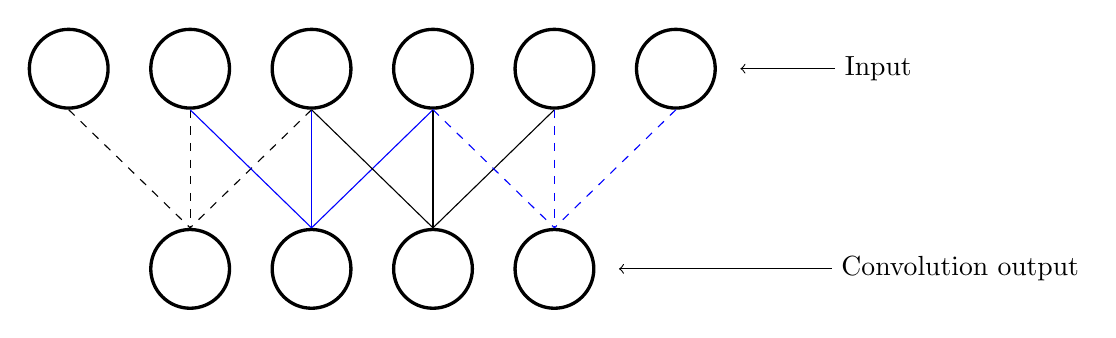
\begin{tikzpicture}[
neuron/.style={circle, draw=black, very thick, minimum size=1cm, transform shape},
dot/.style={circle, draw=black, fill=black, minimum size=0.1cm, inner sep=0pt, transform shape},
note/.style={circle, draw=black, minimum size=0pt, inner sep=0pt, transform shape},
]

%Layer 1 neurons
\node[neuron] (l11) {};
\node[neuron] (l12) [right=0.5cm of l11] {};
\node[neuron] (l13) [right=0.5cm of l12] {};
\node[neuron] (l14) [right=0.5cm of l13] {};
\node[neuron] (l15) [right=0.5cm of l14]{};
\node[neuron] (l16) [right=0.5cm of l15] {};

%Layer 2 neurons
\node[neuron] (l21) [below=1.5cm of l12] {};
\node[neuron] (l22) [below=1.5cm of l13] {};
\node[neuron] (l23) [below=1.5cm of l14] {};
\node[neuron] (l24) [below=1.5cm of l15] {};

%Labels
\node (label_1) [right=1.5cm of l16] {Input};
\node (label_2) [right=3cm of l24] {Convolution output};

%Markers
\node (m1) [right=0.05cm of l16] {};
\node (m2) [right=0.05cm of l24] {};

%Connections Layer 1 - Layer 2
\draw[dashed] (l11.south) -- (l21.north);
\draw[dashed] (l12.south) -- (l21.north);
\draw[dashed] (l13.south) -- (l21.north);

\draw[blue] (l12.south) -- (l22.north);
\draw[blue] (l13.south) -- (l22.north);
\draw[blue] (l14.south) -- (l22.north);

\draw (l13.south) -- (l23.north);
\draw (l14.south) -- (l23.north);
\draw (l15.south) -- (l23.north);

\draw[dashed, blue] (l14.south) -- (l24.north);
\draw[dashed, blue] (l15.south) -- (l24.north);
\draw[dashed, blue] (l16.south) -- (l24.north);

%Marker arrows
\draw[->] (label_1) -- (m1);
\draw[->] (label_2) -- (m2);
\end{tikzpicture}
\caption[Convolution 1D]{Example of a convolution layer with a kernel size of $3$. It highlights the sparse connectivity of the different neurons. Each of the output neurons is now only connected to three of the previous neurons. Each of the weights associated with the lines in the picture above is shared, i.e. the leftmost line (independant of its style and color) always represents the same weight. The same is true for the middle and right line in each of the groups. The size of the output is reduced due to the filter having a kernel size $>1$.}\label{fig:simple_convolution}
\end{figure}
\begin{figure}
\centering
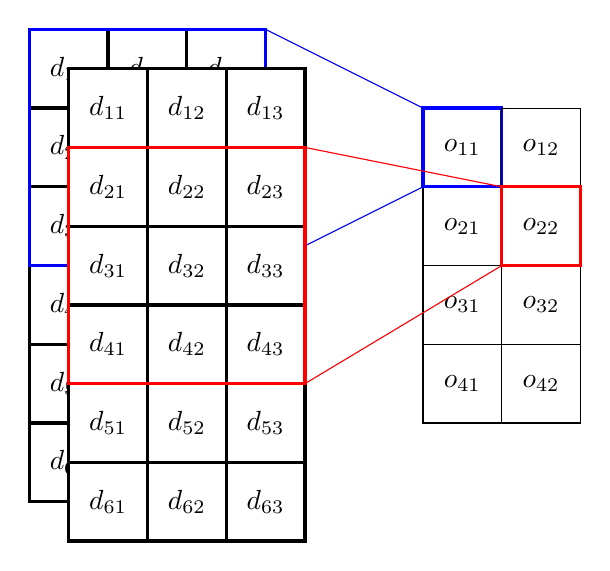
\begin{tikzpicture}[
neuron/.style={circle, draw=black, very thick, minimum size=1cm, transform shape},
dot/.style={circle, draw=black, fill=black, minimum size=0.1cm, inner sep=0pt, transform shape},
note/.style={circle, draw=black, minimum size=0pt, inner sep=0pt, transform shape},
]
\begin{pgfonlayer}{bg}
	\draw[black, very thick] (0,0) rectangle (1,-1) node[pos=0.5] {$d_{11}$};
	\draw[black, very thick] (0,-1) rectangle (1,-2) node[pos=0.5] {$d_{21}$};
	\draw[black, very thick] (0,-2) rectangle (1,-3) node[pos=0.5] {$d_{31}$};
	\draw[black, very thick] (0,-3) rectangle (1,-4) node[pos=0.5] {$d_{41}$};
	\draw[black, very thick] (0,-4) rectangle (1,-5) node[pos=0.5] {$d_{51}$};
	\draw[black, very thick] (0,-5) rectangle (1,-6) node[pos=0.5] {$d_{61}$};
	
	\draw[black, very thick] (1,0) rectangle (2,-1) node[pos=0.5] {$d_{12}$};
	\draw[black, very thick] (1,-1) rectangle (2,-2) node[pos=0.5] {$d_{22}$};
	\draw[black, very thick] (1,-2) rectangle (2,-3) node[pos=0.5] {$d_{32}$};
	\draw[black, very thick] (1,-3) rectangle (2,-4) node[pos=0.5] {$d_{42}$};
	\draw[black, very thick] (1,-4) rectangle (2,-5) node[pos=0.5] {$d_{52}$};
	\draw[black, very thick] (1,-5) rectangle (2,-6) node[pos=0.5] {$d_{62}$};
	
	\draw[black, very thick] (2,0) rectangle (3,-1) node[pos=0.5] {$d_{13}$};
	\draw[black, very thick] (2,-1) rectangle (3,-2) node[pos=0.5] {$d_{23}$};
	\draw[black, very thick] (2,-2) rectangle (3,-3) node[pos=0.5] {$d_{33}$};
	\draw[black, very thick] (2,-3) rectangle (3,-4) node[pos=0.5] {$d_{43}$};
	\draw[black, very thick] (2,-4) rectangle (3,-5) node[pos=0.5] {$d_{53}$};
	\draw[black, very thick] (2,-5) rectangle (3,-6) node[pos=0.5] {$d_{63}$};	
	
	\draw[blue, very thick] (0,0) rectangle (3, -3);
	
	\draw[blue] (3,  0) -- (5, -1);
	\draw[blue] (3, -3) -- (5, -2);
\end{pgfonlayer}

\filldraw[fill=white, draw=black, very thick] (0.5, -0.5) rectangle (1.5, -1.5) node[pos=0.5] {$d_{11}$};
\filldraw[fill=white, draw=black, very thick] (0.5, -1.5) rectangle (1.5, -2.5) node[pos=0.5] {$d_{21}$};
\filldraw[fill=white, draw=black, very thick] (0.5, -2.5) rectangle (1.5, -3.5) node[pos=0.5] {$d_{31}$};
\filldraw[fill=white, draw=black, very thick] (0.5, -3.5) rectangle (1.5, -4.5) node[pos=0.5] {$d_{41}$};
\filldraw[fill=white, draw=black, very thick] (0.5, -4.5) rectangle (1.5, -5.5) node[pos=0.5] {$d_{51}$};
\filldraw[fill=white, draw=black, very thick] (0.5, -5.5) rectangle (1.5, -6.5) node[pos=0.5] {$d_{61}$};

\filldraw[fill=white, draw=black, very thick] (1.5, -0.5) rectangle (2.5, -1.5) node[pos=0.5] {$d_{12}$};
\filldraw[fill=white, draw=black, very thick] (1.5, -1.5) rectangle (2.5, -2.5) node[pos=0.5] {$d_{22}$};
\filldraw[fill=white, draw=black, very thick] (1.5, -2.5) rectangle (2.5, -3.5) node[pos=0.5] {$d_{32}$};
\filldraw[fill=white, draw=black, very thick] (1.5, -3.5) rectangle (2.5, -4.5) node[pos=0.5] {$d_{42}$};
\filldraw[fill=white, draw=black, very thick] (1.5, -4.5) rectangle (2.5, -5.5) node[pos=0.5] {$d_{52}$};
\filldraw[fill=white, draw=black, very thick] (1.5, -5.5) rectangle (2.5, -6.5) node[pos=0.5] {$d_{62}$};

\filldraw[fill=white, draw=black, very thick] (2.5, -0.5) rectangle (3.5, -1.5) node[pos=0.5] {$d_{13}$};
\filldraw[fill=white, draw=black, very thick] (2.5, -1.5) rectangle (3.5, -2.5) node[pos=0.5] {$d_{23}$};
\filldraw[fill=white, draw=black, very thick] (2.5, -2.5) rectangle (3.5, -3.5) node[pos=0.5] {$d_{33}$};
\filldraw[fill=white, draw=black, very thick] (2.5, -3.5) rectangle (3.5, -4.5) node[pos=0.5] {$d_{43}$};
\filldraw[fill=white, draw=black, very thick] (2.5, -4.5) rectangle (3.5, -5.5) node[pos=0.5] {$d_{53}$};
\filldraw[fill=white, draw=black, very thick] (2.5, -5.5) rectangle (3.5, -6.5) node[pos=0.5] {$d_{63}$};

\draw[black] (5, -2) rectangle (6, -3) node[pos=0.5] {$o_{21}$};
\draw[black] (5, -3) rectangle (6, -4) node[pos=0.5] {$o_{31}$};
\draw[black] (5, -4) rectangle (6, -5) node[pos=0.5] {$o_{41}$};
\draw[black] (5, -1) rectangle (6, -2) node[pos=0.5] {$o_{11}$};
\draw[blue, very thick] (5, -1) rectangle (6, -2);

\draw[black] (6, -2) rectangle (7, -3) node[pos=0.5] {$o_{22}$};
\draw[black] (6, -3) rectangle (7, -4) node[pos=0.5] {$o_{32}$};
\draw[black] (6, -4) rectangle (7, -5) node[pos=0.5] {$o_{42}$};
\draw[black] (6, -1) rectangle (7, -2) node[pos=0.5] {$o_{12}$};
\draw[red, very thick] (6, -2) rectangle (7, -3);

\draw[red, very thick] (0.5, -1.5) rectangle (3.5, -4.5);

\draw[red] (3.5, -1.5) -- (6, -2);
\draw[red] (3.5, -4.5) -- (6, -3);
\end{tikzpicture}
\caption[Convolution multiple channels]{Depiction of a convolution layer with two filters, that have a kernel size of $3$. The input data $d_{11}$ to $d_{62}$ has two channels and is the same for both the blue and the red filter. The first channel of the output ($o_{11}$ to $o_{41}$) is produced by sliding the blue filter over the data, the second channel ($o_{12}$ to $o_{42}$) is produced by sliding the red filter over the data. Notice that the filters span all channels of the input data and only slide in 1 dimension.}\label{fig:convolution_channels}
\end{figure}
\begin{figure}
\centering
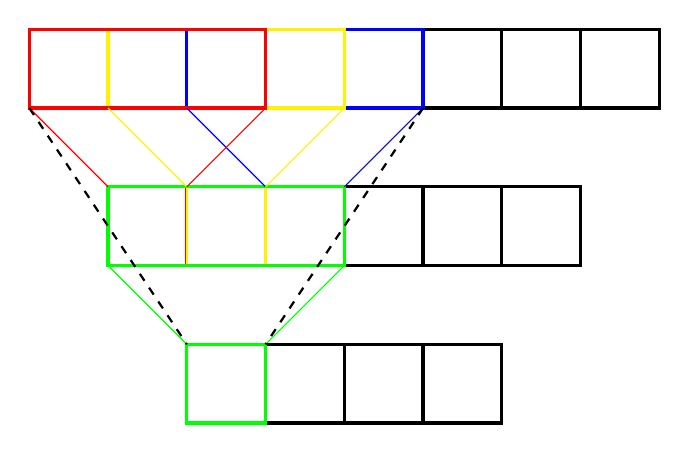
\begin{tikzpicture}[
neuron/.style={circle, draw=black, very thick, minimum size=1cm, transform shape},
dot/.style={circle, draw=black, fill=black, minimum size=0.1cm, inner sep=0pt, transform shape},
note/.style={circle, draw=black, minimum size=0pt, inner sep=0pt, transform shape},
]
%Layer 1
\draw[black, very thick] (0,  0) rectangle (1, -1);
\draw[black, very thick] (1,  0) rectangle (2, -1);
\draw[black, very thick] (2,  0) rectangle (3, -1);
\draw[black, very thick] (3,  0) rectangle (4, -1);
\draw[black, very thick] (4,  0) rectangle (5, -1);
\draw[black, very thick] (5,  0) rectangle (6, -1);
\draw[black, very thick] (6,  0) rectangle (7, -1);
\draw[black, very thick] (7,  0) rectangle (8, -1);

%Filter boxes layer 1
\draw[blue, very thick] (2,  0) rectangle (5, -1);
\draw[yellow, very thick] (1, 0) rectangle (4, -1);
\draw[red, very thick] (0, 0) rectangle (3, -1);

%Layer 2
\draw[red, very thick] (1, -2) rectangle (2, -3);
\draw[blue, very thick] (3, -2) rectangle (4, -3);
\draw[yellow, thick] (2, -2) rectangle (3, -3);
\draw[black, very thick] (4, -2) rectangle (5, -3);
\draw[black, very thick] (5, -2) rectangle (6, -3);
\draw[black, very thick] (6, -2) rectangle (7, -3);

%Filter box layer 2
\draw[green, very thick] (1, -2) rectangle (4, -3);

%Layer 3
\draw[black, very thick] (3, -4) rectangle (4, -5);
\draw[black, very thick] (4, -4) rectangle (5, -5);
\draw[black, very thick] (5, -4) rectangle (6, -5);
\draw[green, very thick] (2, -4) rectangle (3, -5);

%Connections layer 1 -- layer 2
\draw[blue] (2, -1) -- (3, -2);
\draw[blue] (5, -1) -- (4, -2);
\draw[yellow] (1, -1) -- (2, -2);
\draw[yellow] (4, -1) -- (3, -2);
\draw[red] (0, -1) -- (1, -2);
\draw[red] (3, -1) -- (2, -2);

%Connections layer 2 -- layer 3
\draw[green] (1, -3) -- (2, -4);
\draw[green] (4, -3) -- (3, -4);

%Receptive field connections
\draw[black, dashed, thick] (0, -1) -- (2, -4);
\draw[black, dashed, thick] (5, -1) -- (3, -4);
\end{tikzpicture}
\caption[Receptive field]{Three stacked convolution layers. Although all layers have a kernel size of $3$, the final layer is influenced by $5$ of the input values. Therefore the receptive field of the final layer is $5$. \textcolor{red}{Maybe change the colors and some presentation of this graphic. I don't like how it looks.}}\label{fig:receptive_field}
\end{figure}

\subsubsection{Pooling Layers}\label{sec:pooling_layers}
\textcolor{blue}{Explain what max pooling does and why it is useful, even when it is counter intuitive.}
Pooling layers are another special kind of layers, often used to increase performance of \gls{cnns}. Though there are many variations of the specific implementation, the core concept is grouping multiple activations of a single feature map into one activation. The most common pooling layer is the maximum pooling layer, as it puts greater emphasis on strong activations. \cite{max_pooling_invention} It works by grouping a certain number of input activations of the previous layer and assigning this group the maximum values of all the grouped neurons. (see \autoref{fig:max_pooling})\\
Though it does seems counter intuitive, that throwing away information helps the networks performance, the reasons are manifold. First of all pooling in general downsamples the data\footnote{There have been studies suggesting, that pooling works better than simply sub sampling the data. \cite{pooling_vs_subsampling}}. The lower number of datapoints results in fewer calculations per forward pass, fewer trainable parameters being used and thus less overfitting. Secondly, maximum pooling increases the impact of strong activations. These strong activations usually come from the parts of the data that resonate strongly with a convolution filter. If this resonance only applies for a small region in the data, there will only be few values on the feature map, that correspond to this resonance. Therefore pooling (in general) leads to greater spatial invariance. The downside of pooling is the loss of positional information. As a rule of thumb, pooling is useful for a decision ''is a feature present'', but falls short if the question ''where in the data is the feature present'' is also relevant.\\
Due to its improvement in spatial invariance, pooling also leads to the next layer having a greater receptive field.\medskip\\
All the actions described above act only on a single feature map, channel by channel. A similar approach can however also be taken for the channels themselves. Such a procedure is called \emph{dimensional reduction} and usually done through a convolution layer with a kernel size of $1$. This way, all channels are being connected through a weighted sum, where the weights are learned.\cite{dim_red_invention} Additionally a activation function can be used to introduce non-linear  combinations of the channels. In this way, dimensional reduction can not only be seen as a reduction in learnable parameters, but also as means to combine features of different channels. \cite{dim_red_interpretation} As the different feature maps are added together, this operation combines low level features into higher level ones.\\
The number of outgoing channels is given by the number of filters used in the convolution layer with kernel size $1$.
\begin{figure}
\centering
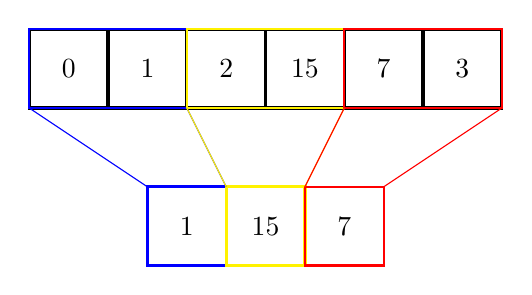
\begin{tikzpicture}[
neuron/.style={circle, draw=black, very thick, minimum size=1cm, transform shape},
dot/.style={circle, draw=black, fill=black, minimum size=0.1cm, inner sep=0pt, transform shape},
note/.style={circle, draw=black, minimum size=0pt, inner sep=0pt, transform shape},
]
%Input
\draw[black, very thick] (0,  0) rectangle (1, -1) node[pos=0.5] {0};
\draw[black, very thick] (1,  0) rectangle (2, -1) node[pos=0.5] {1};
\draw[black, very thick] (2,  0) rectangle (3, -1) node[pos=0.5] {2};
\draw[black, very thick] (3,  0) rectangle (4, -1) node[pos=0.5] {15};
\draw[black, very thick] (4,  0) rectangle (5, -1) node[pos=0.5] {7};
\draw[black, very thick] (5,  0) rectangle (6, -1) node[pos=0.5] {3};

%Filter boxes layer 1
\draw[blue, thick] (0,  0) rectangle (2, -1);
\draw[yellow, thick] (2, 0) rectangle (4, -1);
\draw[red, thick] (4, 0) rectangle (6, -1);

%Layer 2
\draw[blue, very thick] (1.5, -2) rectangle (2.5, -3) node[pos=0.5, black] {1};
\draw[yellow, very thick] (2.5, -2) rectangle (3.5, -3) node[pos=0.5, black] {15};
\draw[red, thick] (3.5, -2) rectangle (4.5, -3) node[pos=0.5, black] {7};

%Connections layer 1 -- layer 2
\draw[blue] (0, -1) -- (1.5, -2);
\draw[blue] (2, -1) -- (2.5, -2);
\draw[yellow] (2, -1) -- (2.5, -2);
\draw[yellow] (4, -1) -- (3.5, -2);
\draw[red] (4, -1) -- (3.5, -2);
\draw[red] (6, -1) -- (4.5, -2);
\end{tikzpicture}
\caption[Max Pooling layer]{An example of a Max pooling layer. It groups together two entries of its input and returns the maximum, thus halving the number of samples per feature map. This process is applied for all channels.}\label{fig:max_pooling}
\end{figure}

\subsubsection{Inception Module}\label{sec:inception_module}
\textcolor{blue}{Explain what it is, how it works. (cite google paper) ONLY IF IT IS REALLY USED IN THE FINAL ARCHITECTURE!}\\
Networks consisting of stacked convolution layers as introduced in \autoref{sec:convolution_layer} have had great success in image classification. \cite{deep_learning_book, alex_net, ILSVRC15} As the field of computer vision is one of the most prominent in machine learning and shows great advances, we use networks successfully applied there as a guideline for new architectures. Accordingly the module showcased in this section was developed for image classification and introduced in \cite{inception_module}.\\
The advantages of convolution layers over classical dense layers are manifold and discussed in further detail in \autoref{sec:convolution_layer}. One of the key advantages however is the comparatively low number of trainable parameters, as the connections are a lot more sparse. The number of these trainable parameters however is still quite large and limits the depth of a Deep-\gls{cnn}. This becomes especially obvious, when one scales the number of filters used in the convolution layers, throughout the network. If the number of filters of two consecutive convolution layers is scaled by a factor $c$, the number of trainable parameters increases by a factor of $c^2$. Scaling the number of filters is one way to increase the capacity of a network and reduce underfitting. \cite{inception_module} Another way to increase the capactity is to scale the convolution-kernel size. \textcolor{red}{Need to talk about over- and underfitting, model capacity and training data differences in a section before this one! (Probably best after the backprop section)} Larger kernels furthermore provide the capabiltiy to detect larger features within a certain part of the image. If they are too large however, the filter might be close to zero for a lot of the learnable parameters, which in turn wastes a lot of computational resources. In this situation an approach that utilizes sparse matrices or tensors would be quite beneficial, if the computational infrastructure supports it efficiently. The advantage gained by the lowered number of computations is however mostly outweight by the computational overhead created. Therefore sparse matrix operations are not feasible at the moment. \cite{inception_module}\\
A workaround for this problem is grouping multiple sparse operations together into matrices that are mostly sparse but contain dense submatrices. The matrix-operations can than be performed efficiently on the sparse matrices, by utilizing the efficient dense operations on the dense submatrices. This is the approach, the inception modules tries to take. They build a single module, that can be viewed as a layer from the outside. It contains multiple small convolution layers, that build up a larger, sparse filter. Using this new architecture, the GoogLeNet won the 2014 \gls{ilsvrc}\footnote{The \gls{ilsvrc} is a yearly competition for computer vision algorithms. It is widely used as a benchmark to judge how well a network (or any other computer vision software) does. It is always the same set of images, where each image belongs to one of about 1000 classes. The top 5 error rate is the relative number of times, the algorithm in use did not return the correct category within its top 5 choices.} image recognition competition in the category ''image classification and localization'', setting a new record for the top 5 error rate, thus proving the effectiveness of the new module. \cite{inception_module, ILSVRC15}\\
As the original work was used to handle 2 dimensional images and thus used 2D-convolutions, the module had to be slightly adjusted to fit the 1 dimensional requirements of the time series data in this work. This was a simple task however, as the difference between the two is simply the shape of the kernel and the way it is moved across the data. With Keras, there are predefined functions to handle 1D and 2D convolutions. The downside of converting the 2 dimensional inception module to a 1 dimensional one however is, that many of the incremental improvements to the module are not applicable, as they rely heavily on the 2D-structure. \cite{inception_v2_v3, inception_v4}\medskip\\
The following paragraphs will describe the module used in this work in greater detail.\\
The module consists of 4 independent towers, each consisting of different layers. The full module is depicted in \autoref{fig:inception_module}.\\
The module consists of three parallel convolution layers, i.e. each of the three layers share the same input. The difference between them is the kernel size. The convolution layers with a larger kernel a preceded by a convolution layer with $16$ filters and a kernel size of $1$. The purpose of this step is to reduce the number of channels used and is called dimensional reduction. This leads to a fixed input size for the larger kernels, regardless of the depth of the input. 
In the original architecture filters of size $1\times1$, $3\times3$ and $5\times5$ were used. Translating them directly to 1 dimensional equivalents, the module should use kernel sizes of $1$, $3$ and $5$. However we empirically found, that the smallest kernel sizes $1$, $2$ and $3$ performed best. \textcolor{red}{(Did I ever try 1,3,5? If not do so!)}\\
Finally a pooling layer as introduced in \autoref{sec:pooling_layers} is added as a fourth path. The reasoning behind this step is, that pooling layers have shown great improvements in traditional \gls{cnns} and thus the network should be provided with the option to choose this route as well. For this layer the dimensional reduction takes place only after the pooling procedure.\\
The output of each of these paths is than concatenated along the last axis of the tensor, i.e. along the different channels. For this reason all input to each of the layers is padded with zeros in such a way, that the shape (except for the channels) does not change.
\begin{figure}
\centering
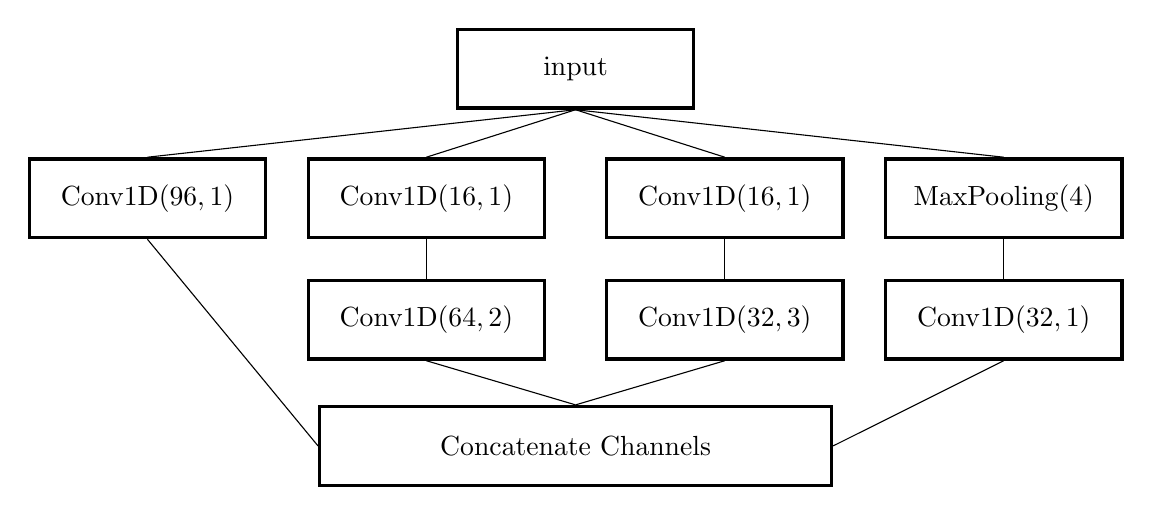
\begin{tikzpicture}[
neuron/.style={circle, draw=black, very thick, minimum size=1.0cm},
dot/.style={circle, draw=black, fill=black, minimum size=0.1cm, inner sep=0pt},
VLineVertex/.style={circle, draw=black, minimum size=0cm, inner sep=0pt},
layer/.style={rectangle, draw=black, very thick, minimum height=1cm, minimum width=3cm},
concat/.style={rectangle, draw=black, very thick, minimum height=1cm, minimum width=6.5cm}
]

%Nodes
\node[layer] (input) {input};
\node (midpoint) [below=1cm of input] {};
\node[layer] (l_2_dim_red) [left=0.25cm of midpoint] {Conv1D$\lr{16, 1}$};
\node[layer] (l_2_filter) [below=0.5cm of l_2_dim_red] {Conv1D$\lr{64, 2}$};
\node[layer] (l_1) [left=0.5cm of l_2_dim_red] {Conv1D$\lr{96,1}$};
\node[layer] (r_2_dim_red) [right=0.25 of midpoint] {Conv1D$\lr{16, 1}$};
\node[layer] (r_2_filter) [below=0.5cm of r_2_dim_red] {Conv1D$\lr{32, 3}$};
\node[layer] (r_1_pool) [right=0.5cm of r_2_dim_red] {MaxPooling$\lr{4}$};
\node[layer] (r_1_dim_red) [below=0.5cm of r_1_pool] {Conv1D$\lr{32, 1}$};
\node[concat] (concat) [below=2.5cm of midpoint] {Concatenate Channels};

%Connections
\draw (input.south) -- (l_1.north);
\draw (input.south) -- (l_2_dim_red.north);
\draw (input.south) -- (r_2_dim_red.north);
\draw (input.south) -- (r_1_pool.north);

\draw (l_2_dim_red.south) -- (l_2_filter.north);
\draw (r_2_dim_red.south) -- (r_2_filter.north);
\draw (r_1_pool.south) -- (r_1_dim_red.north);

\draw (l_1.south) -- (concat.west);
\draw (l_2_filter.south) -- (concat.north);
\draw (r_2_filter.south) -- (concat.north);
\draw (r_1_dim_red.south) -- (concat.east);
\end{tikzpicture}
\caption[Inception module]{Shown are the contents and connections of the inception module as used in this work. \textcolor{red}{(If the filter numbers and values change for the final architecture, change them here too.)} The layer Conv1D$\lr{x,y}$ is a 1 dimensional convolution layer with $x$ filters and a kernel size of $y$. Most of the convolution layers with a kernel size of $1$ are used for dimensional reduction. The only exception is the leftmost one, that consists of $96$ filters. The different filter sizes correspond to the ability of detecting features at different scales. The pooling layer is a 1 dimensional pooling layer, that only passes on the maximum value in a bin of size 4. The final layer concatenates the channels of the different towers. This also means, that each tower needs to have the same output-shape, excluding the channels. For this reason all inputs are automatically padded with zeros in such a way, that the output-shapes are correct.}\label{fig:inception_module}
\end{figure}

\subsubsection{Temporal Convolutional Networks}
\textcolor{blue}{Explain what they are, what their advantages are and list works that utilized them.}
Temporal convolutional networks (\gls{tcn}), as used in this work, were proposed by \cite{tcn_paper}. Their research suggests that this specialized \gls{cnn}-architecture outperforms \gls{rnns}, which were previously the norm for analyzing and processing sequence data.\\
A \gls{tcn} basically consists of multiple stacked convolution layers, that are slightly adapted in two different ways. For once, the filters are diluted, meaning, that the weighted sum of the convolution is not taken over successive input points. Instead the weighted sum uses points, skipping a set number of inputs in between. Secondly the connections are causal. This means, that output $y_i$ of the filter depends at most only on points $x_i, \dotsc,x_1$. Finally the input of each such layer is padded with zeros such, that the output matches the size of the input. (see (a) of \autoref{fig:tcn})\\
The advantage of the dilated convolution layers is, that the receptive field of the network grows exponentially with the depth, whereas without the dilution this growth is only linear. \textcolor{red}{[Citation]} The goal of the \gls{tcn} is to have a receptive field, that spans the entire input length. This still requires a decently deep network for inputs of considerable length. To combat the problem of the vanishing gradient, residual connections are also introduced. The dimensional reduction layer that is part of the residual connection is simply used to adjust the number of channels to be able to add the input and the output of the residual block together. The full structure of the residual block is shown in (b) of \autoref{fig:tcn}. The only adaption to the implementation that this work makes is the the replacement of the WeightNorm layer with a traditional BatchNormalization layer, as it is described in \autoref{sec:batch_norm}. This is done for convenience, as there is a pre-implemented version of batch normalization in the software library used. This replacement is valid, as weight normalization is described by the authors to be largely a fast approximation to full batch normalization. \cite{weigth_norm_invention}
\begin{figure}
\centering
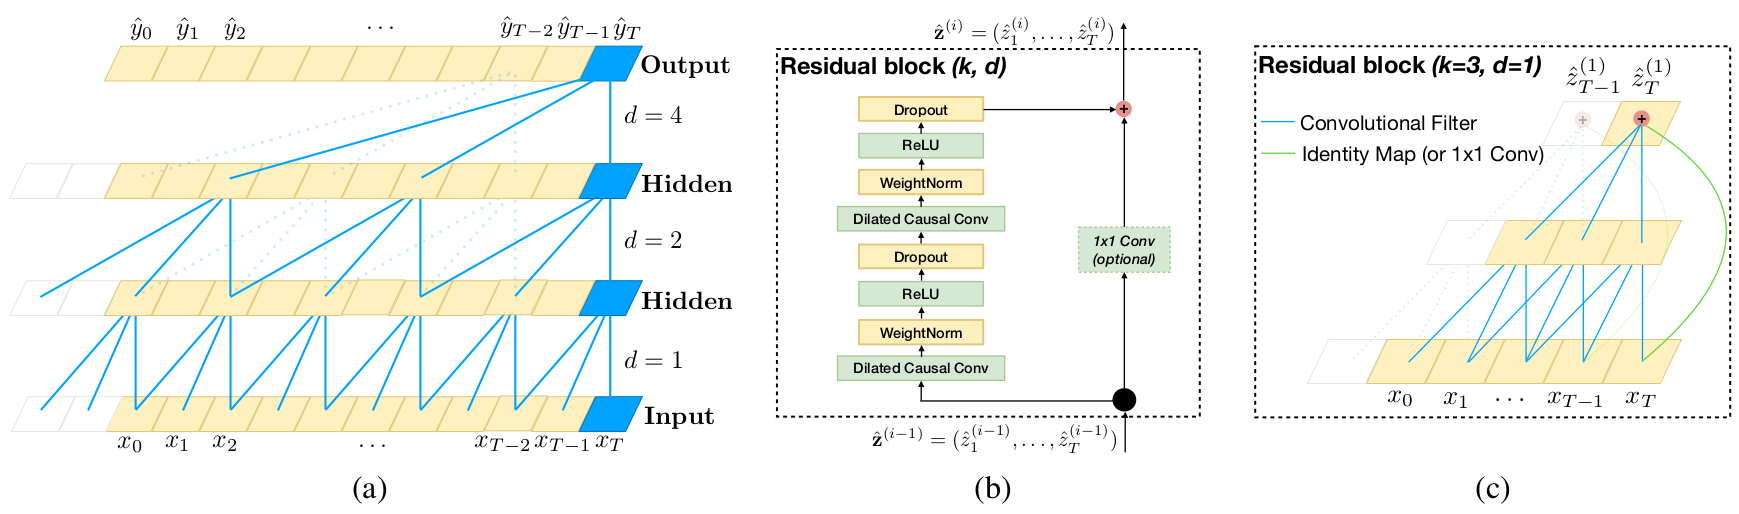
\includegraphics[width=\textwidth]{TCN.png}
\caption[TCN structure]{Architectural elements in a \gls{tcn}. Graphic taken from \cite{tcn_paper}. (a) Exponential increase of the receptive field in diluted convolution layers. Here the dilution factor $d$ scales as $2^i$ and the kernel size $k$ is set to $3$. The causal structure propagates through the layers, as no output is connected to an earlier input. (b) Multiple different layers are utilized for an entire module of the \gls{tcn}. Also a residual connection is used, to help earlier levels learn. Multiple of these units are stacked to form a \gls{tcn}. (c) An example of how the residual block from (b) could look like.}\label{fig:tcn}
\end{figure}


\subsection{Regularization}\label{sec:regularization}
As \cite{deep_learning_book} put it: ''Regularization is any modification we make to a learning algorithm that is intended to reduce its generalization error but not its training error.''. There are many ways, like reducing the number of trainable parameters or adjusting the loss function to prefer specific weights, to achieve this goal. This section however will only introduce two specialized methods, that are introduced as a layer into the network.

\subsubsection{Batch Normalization Layer}\label{sec:batch_norm}
\textcolor{blue}{Explain how batch normalization works and why it is useful. (cite according paper)}
Batch normalization was introduced in \cite{batch_normalization_invention} and is used to normalize the inputs of each layer. This helps the network learn faster and generalize more easily.\\
The normalization tries to fix the distribution of the inputs between different samples, as the layers would need to adapt their weights otherwise for different input distributions. Specifically the goal is to transform the data in a way, that the mean is $0$ and the variance is $1$. Normalizing data in such a way is in principle not problematic and a standard procedure only for the input layer. \textcolor{red}{[Citation]} The problem of normalizing the input of each individual layer is the backporpagation step, as it can lead to exploding biases. \cite{batch_normalization_invention}\\
To solve this issue, gradients of the normalization with respect to multiple inputs need to be computed. Batch normalization uses the samples of each mini-batch to compute the mean, variance and gradients. To reduce computational cost, the normalization is computed only over one dimension of the input. In this work, the mean and variance will be calculated for every channel and thus applied to each channel individually. Finally a linear transformation
\begin{equation}
y_i = \gamma \hat{x}_i + \beta
\end{equation}
is applied to the normalized data
\begin{equation}
\hat{x}_i = \frac{x_i - \mu_B}{\sqrt{{\sigma_B}^2 + \varepsilon}}.
\end{equation}
Here $x_i$ is the $i$-th sample of the mini-batch, $\mu_B$ is the mean and ${\sigma_B}^2$ is the variance of the activations calculated over the mini-batch. The factors $\beta$ and $\gamma$ are learned parameters and $\epsilon$ is a constant added for numerical stability.\\
The linear transformation is applied so that the batch normalization layer can learn to be the identity transformation. Otherwise the normalization could loose the ability to represent some function it previously could have represented.\medskip\\
The implementation in Keras differs from this approach in the sense, that the mean $\mu_B$ and variance ${\sigma_B}^2$ are only calculated for each individual batch during training. When the network is used to evaluate some data, it will use a fixed mean and variance, that was approximated over all batches during training. They call this the moving average $\mu_\text{mov}$ and moving variance $\sigma_\text{mov}^2$ respectively and adjust them after every batch by
\begin{align}
{\mu'}_\text{mov} & = m\cdot\mu_\text{mov} + \lr{1-m}\mu_B\nonumber\\
{{\sigma'}_\text{mov}}^2 & = m\cdot{\sigma_\text{mov}}^2 + \lr{1-m}{\sigma_B}^2,
\end{align}
where $m$ is the momentum used and usually set to a high value around $0.99$. Using this has the advantage, that only a finite number of samples have a non negligible effect on the mean- and variance value used during inference. Therefore drifts in the input distribution, which might occur during training, can be counteracted.

\subsubsection{Dropout Layer}
\textcolor{blue}{Explain what a dropout layer is, what it does, why it is useful.}\\
Dropout layers were introduced in 2014 by \cite{dropout_invention} and showed great improvements to lowering the generalization error. It works by dropping a random percentage of neurons from the network during training. Though this approach sounds counter intuitive, it has multiple benefits.\\
One viewpoint is using the dropout layer as a noise source for the network. By dropping some activations during training, the network can't be too strongly dependent on a single connection and has to learn multiple ways of detecting some feature. Therefore the network becomes less sensitive to small alterations of the input. Furthermore the dropout layer can be used as a first layer in a network and act as data augmentation, where it introduces further noise to the data, as  the same sample may experience different dropped connections. Therefore the effective number of samples the network sees during training is enlarged.\\
Another viewpoint is, that training a network with dropout layers does not only tryout the full architecture, but also all sub-networks, that can be created from the full architecture by dropping some connections. The number of sub-networks grows exponentially with the number of dropout layers. This viewpoint is the main selling point promoted by \cite{deep_learning_book} and \cite{dropout_invention}, as it allows to efficiently sample many networks and combine them.\\
During the evaluation process, the original paper \cite{dropout_invention} suggests reweighing the weights by the dropout probability, to get an averaging effect. This step is however not done in the software library Keras used in this work. \textcolor{red}{[Citation]}


\section{Network Topologies}\label{sec:network_topologies}
%\textcolor{blue}{The title needs to be improved!\\Explain what we are trying to do once more and how our net achieves that.}\\
\textcolor{red}{Need to introduce the optimizer we are using. Probably should do so in the beginning of the evolution section. Check entire work for ''diluted'' convolution and replace by ''dilated'' convolution.}\\
This section summarizes the results of our research, trying to find a deep learning algorithm that succeeds in detecting and classifying \gls{bns}-signals in noisy data. The goal was to not only classify the signals into the two categories ''pure noise'' and ''signal'' but also to give an estimate of the signals \gls{snr}.\\
%All software written for this work used the PyCBC software package \cite{pycbc} for any code involving gravitational wave data and the deep learning library Keras \cite{keras} to rapidly develop and test different network architectures. We used Tensorflow \cite{tensorflow} as the backend for Keras. \textcolor{red}{Should I cite the libraries here again? I did so in the introduction.}

\subsection{The Data Generating Process}\label{sec:data_generating_process}
%\textcolor{red}{Things missing: Mention training/validation split, mention that we shift the template around in the data (important for why we slide the generator in steps of 0.25s). ATTENTION!!! THE GENERATOR USED FOR THE TESTING SET CURRENTLY USES THE ANALYTIC PSD INSTEAD OF THE WHITEN FUNCTION! THIS IS DISPLAYED DIFFERENTLY IN THE TEXT! CORRECT EITHER THE GENERATOR OR THE TEXT! Take great care to carefully explain multirate filtering.}\\
%\textcolor{blue}{Explain how the data is generated (especially that it only contains gaussian noise). Explain how training/validation set are different from the testing set used in this work. Explain how we carefully chose the parameters, especially how we got the SNR-values. Also explain the mix-and-match approach, that noise can be pure or the same noise with different signals. Also the same signal can (but this isn't necessary) have multiple noise instances. The pure noise SNR was set to 4, as that is the average value for pure noise matched filtering returns. (One might want to alter this) Finally we were careful, that no noise instance or signal from the training set is used in the validation set.}\\
Training a \gls{nn} to detect and classify \gls{bns} signals requires a large set of mock data. Using the data without some processing, however, is not possible. This is due to the fact that \gls{bns} signals are more difficult to train for than \gls{bbh} signals, as they are a lot weaker and last for a longer duration\footnote{\gls{bbh} signals spend about \SI{1}{\s} within the sensitive frequency range of our detectors, whereas \gls{bns} signals can be visible in the whitened detector data for multiple tens of seconds \cite{gw170817} and when generated even last multiple hundred seconds.}. Training a \gls{nn} on data of such duration sampled at a frequency high enough to resolve the final cycles of the binary system is not feasible, as the required network would need too many trainable parameters. However, to retain most of the \gls{snr} in the data, it is not possible to crop it to only contain a small portion of the waveform. To overcome this issue note that even though \gls{bns} signals spend a long time in the sensitive region of the detectors, their frequency evolves rather slowly and starts at low values.\\
For the early inspiral phase of the signal, frequencies are around \SIrange{30}{100}{\hertz}. To resolve these frequencies, a sample rate of \SIrange{60}{200}{\hertz} is necessary. The higher sample rates are only required for the final few seconds. For these reasons we propose to represent the data using a new multi-rate approach. Using this method, the network does not receive the data at a fixed sample rate, but rather multiple inputs, each sampling parts of the signal at different rates.\\
We choose the largest window to encompass \SI{64}{\s} of data, where a signal is aligned such, that the high frequency cutoff is roughly \SI{0.5}{\s} from the end. Afterwards we chop the data into parts of duration \SI[parse-numbers=false]{2^i}{\s} and re-sample each of these parts to have a sample rate of \SI[parse-numbers=false]{2^{12-i}}{\hertz}, with $i=0,\dotsc ,6$. This way each sample rate contains exactly $4096$ samples.\\
The 7 re-sampled data segments, however, have overlaps. This is due to the fact, that the lower sample rates contain the data of the higher sample rates, e.g. the \SI{2}{\s} interval sampled at \SI{2048}{\hertz} also includes the \SI{1}{\s} interval sampled at \SI{4096}{\hertz}. For this reason and to reduce the number of input samples even further, we only use the first $2048$ samples for each rate, except the highest one. To keep things simple however, the highest sample rate is split into two parts, each containing $2048$ samples. Therefore each \SI{64}{\s} input interval is split and re-sampled to yield 8 inputs, each containing $2048$ samples. A depiction of this multi-rate sampling can be found in \autoref{fig:multirate_sampling}.
\begin{figure}
\centering
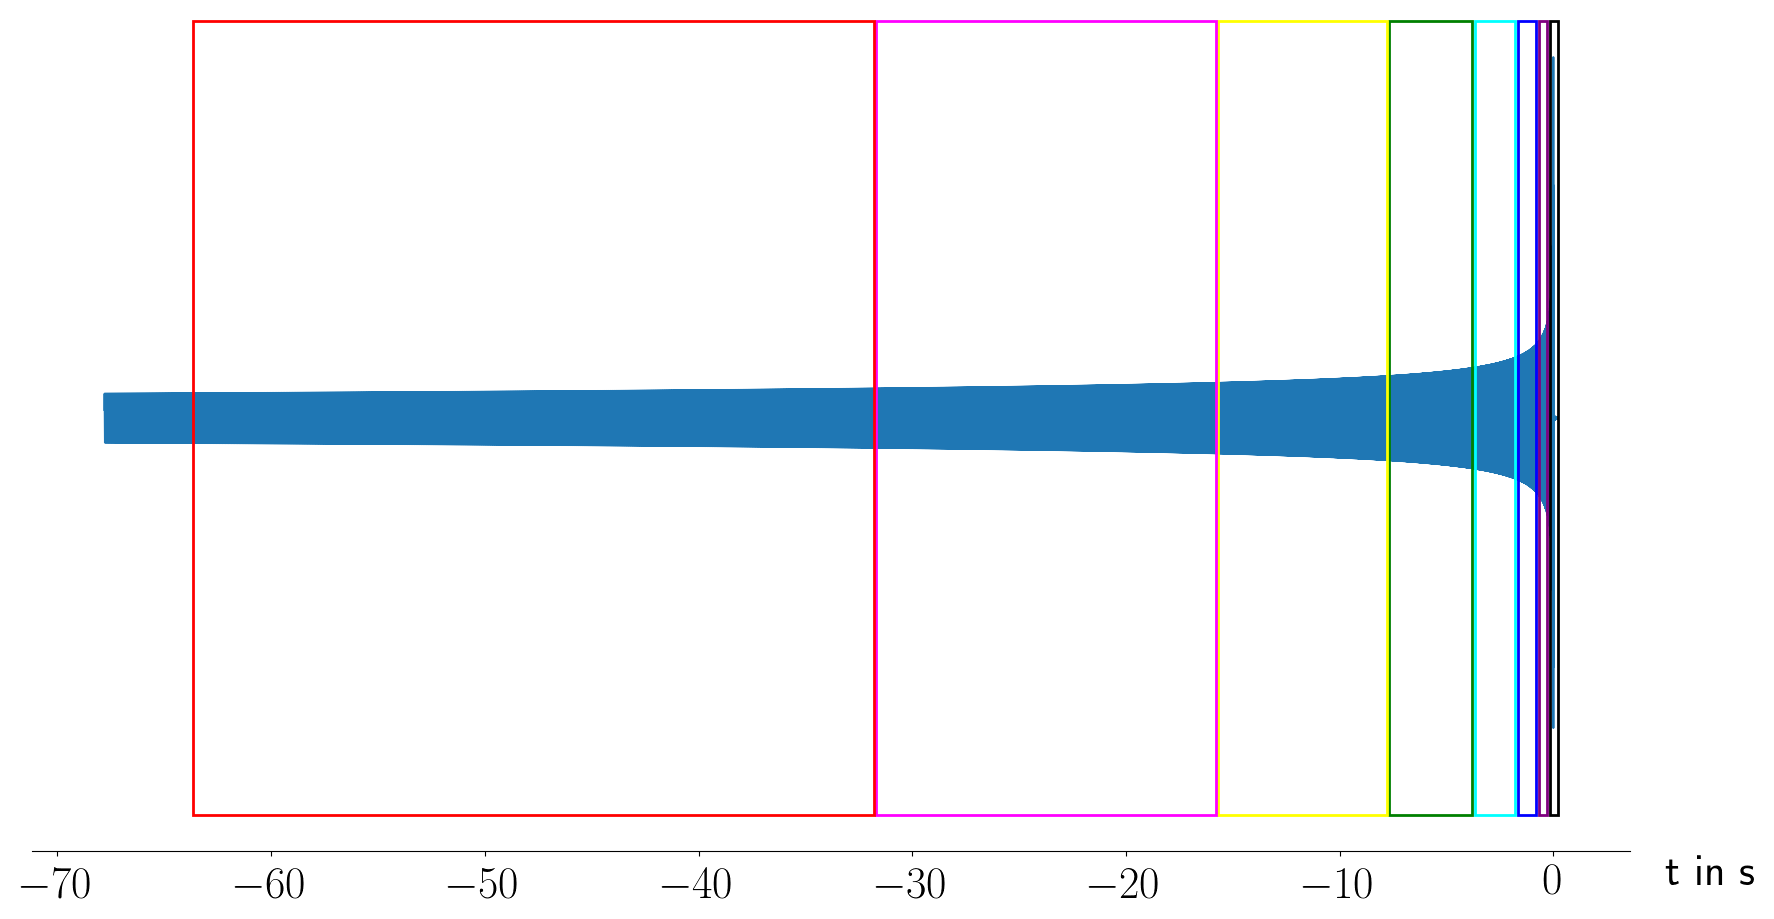
\includegraphics[width=\textwidth]{multirate_filtering_crop.png}
\caption[Multi-rate sampling]{The plot shows how each \gls{bns} signal is sampled at multiple rates. Only the last \SI{68}{\s} of the entire waveform are shown. Each sample rate and interval has its own color attributed. Specifically they are given by: black=(\SI{0.5}{\s}, \SI{4096}{\hertz}), purple=(\SI{0.5}{\s}, \SI{4096}{\hertz}), blue=(\SI{1}{\s}, \SI{2048}{\hertz}), cyan=(\SI{2}{\s}, \SI{4096}{\hertz}), green=(\SI{4}{\s}, \SI{1024}{\hertz}), yellow=(\SI{8}{\s}, \SI{512}{\hertz}), magenta=(\SI{16}{\s}, \SI{256}{\hertz}) and red=(\SI{32}{\s}, \SI{64}{\hertz}), where each tuple gives (segment duration, sample rate).}\label{fig:multirate_sampling}
\end{figure}
\medskip\\
A common drawback of training deep \gls{nns} is the need for large training sets. Luckily we are in a position where we can simulate our training samples and thus can generate an arbitrary amount. To do so we use the PyCBC software package \cite{pycbc}. The final training set contained $56250$ different signals and $161250$ different noise realizations. All of the noise samples were simulated using the analytic \gls{psd} \verb|aLIGOZeroDetHighPower| provided by PyCBC. Therefore all results obtained using this data only hold for stationary gaussian noise. All waveforms were generated using the approximant ''TaylorF2'', as implemented by PyCBC. \textcolor{red}{(Should this be Lal?)} Out of the 17 parameters that could have been varied, we fixed the spins to $0$ and neglected tidal effects for simplicity. Furthermore the coalescence time $t_\text{coal}$ is set to $0$ as well. The remaining $8$ parameters were chosen to represent a realistic distribution in order to estimate the potential of our approach in a real search. As such, both component masses $m_1$ and $m_2$ are uniformly distributed in the range \SIrange{1.2}{1.6}{M_\odot}. Specifically we do not explicitly require $m_1\geq m_2$ when generating the waveform. The coalescence phase $\Phi_0$  and the polarization angle $\psi$ are uniformly distributed on the interval $\left[0, 2\pi\right]$ and the inclination $\iota$ is distributed like $\arccos\lr{\text{uniform}\lr{-1, 1}}$. Finally the sky-position is isotropic, i.e. $\theta$ is distributed like $\arccos\lr{\text{uniform}\lr{-1, 1}}$ and $\varphi$ uniform in $\left[-\pi, \pi\right]$.\\
The luminsoity distance $r$ is chosen indirectly by fixing the \gls{snr} to some value. This is valid, as the \gls{snr} scales inversely with the distance. \textcolor{red}{(Is this true, or is for instance $SNR\approx 1/r^2$?))} In this work, the \gls{snr} is uniformly distributed on the interval $\left[8,15\right]$. One has to avoid one major pitfall when fixing or calculating the \gls{snr} and comparing it to other results. If one compares the \gls{snr} of two signals with the same parameters, the value will depend on the length of the segment used. According to \textcolor{red}{Reference to matched filtering section}, cutting off the waveform early might result in a lower or at least inaccurate value of the \gls{snr}. We therefore specify very precisely how we calculated the \gls{snr}. The waveforms are generated with a lower frequency cutoff of \SI{20}{\hertz}, which results in waveforms, with a duration of about \SI{500}{\s}. Afterwards the waveforms are projected onto the two detectors Livingston and Hanford and cropped in such a way, that they span \SI{96}{\s} and the shutoff lies within the last second. We vary the exact position of the highest amplitude between \SIrange{0.25}{0.75}{\s} from the end of the data stream and choose the signal that arrives at the latest point in time as reference. Only after the waveforms are cropped, we calculate the \gls{snr} of the pure signal (while assuming the \gls{psd} of the detector) using the waveform itself as a template. Since we are using multiple detectors, the \gls{snr} $\rho_i$ is calculated for each detector. The total \gls{snr} in the absence of noise is given by
\begin{equation}
\rho_\text{total} = \sqrt{\sum_i\rho_i^2}.
\end{equation}
Each waveform is than rescaled by multiplying with the factor $\text{\gls{snr}} / \rho_\text{total}$, where \gls{snr} is the target value. Each noise sample is labeled with \gls{snr} $4$ by convention. This value can in principle be picked freely but we chose it to resemble the average output of a matched filter search on pure noise. As a last step, before re-sampling the data as described above, the samples are whitened. To do so, we divide each of them by the amplitude spectral density given by $\sqrt{\text{\gls{psd}}}$. The \gls{psd} again is given by the analytic version \verb|aLIGOZeroDetHighPower| provided by PyCBC. Ideally one would use an estimate of the \gls{psd} to whiten the data. This is, however, not possible in our case, as we are storing signals and noise separately and only add them together at run time. Estimating the \gls{psd} would have the advantage of being more robust in a real search, as it would counteract drifts in the \gls{psd}.\\
The reason for storing noise and signals separately are resource constraints. To cover the entire parameter-space densely enough and avoid overfitting, a large number of samples is necessary. Initially we generated and stored the sum of signal and noise, instead of storing each category separately. This has multiple disadvantages, but also one key advantage; we can use the pure signal as a filter for the matched filtering \textcolor{red}{(Insert equation number here)}, thus  giving us an upper limit on the quality of the \gls{snr} a matched filter search could return. In that sense, we could monitor the performance and compare it to matched filtering directly during training. The disadvantages however at some point outweighed this advantage. The core one being the restricted number of samples. A file containing $500,000$ samples has a of \SI{\sim 200}{\giga\byte}. To train the networks on the data, we completely load it into system memory and need some overhead for formatting. To reduce these costs, we decided to split the signal- and noise-samples and only at runtime add together one instance of each category on the first layer of the network. The second advantage of this approach is less obvious. It enables us to easily feed the network the same signal submerged in multiple different noise realizations, which resulted in performance improvements for tasks similar to ours (Christoph Dreißigacker, personal communication, June 2019).\\
The split between training and validation set is treated with great care, assuring that not a single noise or signal sample from the training set is used during validation. Therefore the reported loss and accuracy values are representative of a real search. Though they are not the final statistic we report, they are tightly linked to those and give clues about the network and its efficiency.\\
The data used for training and validating the final network contained $75,000$ different \gls{gw}-signals and $215,000$ noise realizations\footnote{The numbers stated above were the number of samples in the training set. Here we are stating the numbers for the training and validation set combined, as they are stored in the same file. The numbers for the training set are a results of the split described below.}. We than generate a set number of unique index pairs $(s_i, n_i)$, where $s_i$ corresponds to a signal and $n_i$ to a noise sample. For the training set these indices may be selected from $s_i\in\left[0, 3/4s_t\right)$ and $n_i\in\left[0, 3/4n_t\right)$, where $s_t$ and $n_t$ are the total number of signals and noise samples respectively. If $3/4s_t\notin\mathcal{N}$ or $3/4n_t\notin\mathcal{N}$, the upper index is rounded to the nearest natural number. The total number of pairs generated is equal to the number of usable noise samples $3/4 n_t$. These index pairs represent all samples of the training/validation set that contain a \gls{gw}. In order to also supply pure noise samples to the learning algorithm, all noise realizations are also used during training. This is achieved by appending all index pairs $\lr{-1, 0}, \lr{-1, 1}, \dotsc, \lr{-1, 3/4n_t}$ to the list of index pairs generated before. Afterwards this list is shuffled. The \gls{nn} finally is fed with these $2\cdot 3/4 n_t$ samples through a function\footnote{Keras calls this function a generator.} that interprets the indices and reshapes the data. Overall the training set therefore consists of $322,500$ samples with a $1:1$-split between noise and signals. The validation set does have a $3:1$ split in favor of signals and contains the remaining $n_t / 4$ noise samples. Therefore, the validation set consists of $215,000$ samples.\\
The shape of the data depends on the network in use. Our final network expects a list of $16$ arrays, as we have $8$ different sample rates and a signal and noise input for each of them. The arrays are of shape $\lr{\text{mini-batch size, 2048, 2}}$. The last axis is the number of detectors used, whereas the second axis is the number of samples in the time series strain data.\medskip\\
Above we have only discussed the training and validation set in detail. The final results, however, are evaluated on the testing set. To eliminate most possible error sources, the testing set is generated completely independently from training and validation set, sharing only the distribution of parameters as discussed above. The testing set, furthermore, does not consist of individual samples, where each sample either contains a \gls{gw} aligned correctly or not, but is a set of continuous time series data. These large chunks are then handed to a generator function that chops each time series into overlapping blocks, i.e. sliding a window across the data. Each of these windows has a length of \SI{96}{\s}. The resulting chunk is whitened by dividing out the amplitude spectral density associated to the analytic \gls{psd} \verb|aLIGOZeroDetHighPower| and re-sampled to match the criteria of the network input. The window is than shifted by \SI{0.25}{\s} and the process repeated. The temporal resolution of \SI{0.25}{\s} was chosen because the waveforms are shifted around in the training set by \SI{\pm 0.25}{\s}. With the step chosen this way, we are guaranteed to have the maximum amplitude of the signal in the sensitive window of the network at some point. The result of sliding the network across the input data in the way described results in a \gls{snr} and p-score time series with time resolution \SI{0.25}{\s}. From these triggers can be generated by choosing some threshold based on the findings on the validation set.\\
The testing data was generated by Dr. Alexander Harvey Nitz using PyCBC but utilizing different functions.

\subsection{Evolution of the Architecture}\label{sec:evolution_of_architecture}
%\textcolor{blue}{Talk about the different things we tried, what didn't work and how we improved on them. (Improvement from convolution to inception, improvement from inception to collect-inception, improvement from inception to tcn-inception, improvement of tcn-collect-inception over collect-inception.)}\\
%\textcolor{red}{Talk about the different loss functions used for the two outputs. Also mention their loss weights and training algorithms? Talk about general points we found, i.e. using dropout makes loss a little less stable but improves performance even when a lot of samples are used. (compare (24.06.2019) and (25.06.2019 (1)), (19.06.2019) and (25.06.2019 (2))) Decreasing learning rate in Adam did not help (19.06.2019).}\\
This section gives an overview of the steps that were taken to arrive at the final architecture. It chronologically highlights the pivotal points along the way and showcases some ideas that did not work out.\\
As a starting point we tried to use an easy case, where the \gls{snr} was uniformly distributed between 10 and 50, with all other parameters fixed. The neutron stars were modeled with $m_1=m_2=$ \SI{1.4}{M_\odot}. The data was stored and loaded as the sum of signal and noise and contained data for the two detectors Hanford and Livingston. In general, the data contained samples of signals and pure noise realizations. Until stated otherwise, all of the following networks use this data.\\
To rate the performance of a network we didn't use the sensitivity of the network yet. Instead we used the variance and mean squared error of the recovered \gls{snr}-values compared to the label values in order to estimate performance, hoping that these simple statistics correlate strongly with the actual sensitivity.\medskip\\
The first architecture we used was very close in nature to that of \cite{huerta_parameter_estimation}, halving, however, the number of filters in each convolutional layer and using batch normalization in between the convolution and its activation. Therefore, we used a network of 3 stacked convolutional layers, each followed by a batch normalization, ReLU activation \textcolor{red}{(Never introduced the ReLU activation)} and maximum pooling layer. The number of filters was doubled after each convolutional layer. Since the input data to our network is sampled at multiple rates, this network has 14 input channels instead of 2. (7 input channels per detector, where each of the 7 channels corresponds to a single sample rate)\\
Though initially trained without pure noise samples and with only the \gls{snr} as training goal, we soon changed to use the data as mentioned in the beginning of this section. Furthermore, we added a second output. This second output gives a number between 0 and 1, where 1 corresponds to the network classifying the data as signal and 0 for classifying it as pure noise. If the output is neither 0 nor 1 one can use a threshold to determine if the output should correspond to a signal or pure noise. By default the threshold value is set to $0.5$. We will refer to the results this output gives as ''p-score'' throughout this work, even though it is not really a probability. As this second output tries to categorize the results into two different classes, it is inefficient to use mean squared error as a loss for this output. Instead we use a loss called categorical crossentropy, which is designed to optimize classification problems. As we are using two different losses now, the network will optimize the sum of the mean squared error from the \gls{snr}-output and the categorical crossentropy from the p-score output. This furthermore requires us to split the last layer into two.\\
%All of the following analysis is based purly on (13.02.2019) in \cite{network_wiki} and its limited information. Therefore, a lot of the statements below are only qualitative rather than quantitative.\\
Due to the limited statistics calculated at the time, a lot of the statements below are solely qualitative rather than quantitative.\\
The network was able to recover the \gls{snr} of signals rather well but has a large spread for the recovered \gls{snr} values of pure noise samples. The sensitivity can be eyeballed to reach 100\% only above \gls{snr} $\sim 25$ and dropping close to 0\% below \gls{snr} $\sim 20$. The latter is caused by the high \gls{snr} values assigned to certain noise samples, some reaching values of up to $\sim 20$. Furthermore, evaluating the second output on 3000 signals from the validation set gives an accuracy of about 95\% and a false positive rate of about 6\%. These numbers don't sound terrible but are in context. First of all, signals are expected to be in the \gls{snr}-range of 5-15 \textcolor{red}{[Citation]}. At these values the false positive rate seems to be a lot higher than the 6\% over the entire validation set. Secondly, a false positive rate of 6\% equates to a false alarm rate of about \SI[per-mode=fraction]{6e5}{\samples\per\month}\footnote{This crude calculation uses 0.5 as a threshold value. Therefore, one gets $6\times 10^5$ samples with the output being larger than 0.5 per month.}. Ideally the false alarm rate should not exceed 1 per 2 months above an \gls{snr} of about $8$, as that false alarm rate is the threshold used to alert astronomers \cite{pycbc_live}. A month for this work is defined to be \SI{30}{\days}.\medskip\\
From this point the first major iteration was the introduction of inception modules \cite{inception_module}. They replaced the simple convolutional layers of the architecture used previously.
%(see 15.02.2019 and 03.04.2019 in \cite{network_wiki})
 Furthermore, guided by \cite{inception_module}, the inception modules were preceeded by 2 convolutional layers. The implementation of the inception module was as a first step a direct adaptation of the original work \cite{inception_module}. It used kernel sizes of $\lr{1,3,5}$. With these kernel sizes, results did not improve but rather got worse. Increasing the filter sizes to $\lr{4,8,16}$, however, proved to be a useful change. The performance in mean squared error, variance and false positive rate improved significantly, with the false positive rate reaching $\sim 0.015\%$. By eye, the sensitivity also made an improvement as the loudest false positive was estimated to have \gls{snr} $\sim 15$. With this, the sensitive went up to 100\% around \gls{snr} 20 and only dropped to 0\% below \gls{snr} $\sim 12$. Though this is still not an impressive performance, it is a considerable improvement over the simple convolutional approach.\medskip\\
Having found the new inception architecture, we conducted a test to figure out which of the 7 sample rates benefit the network the most.
% To view the full results see 04.04.2019 and 05.04.2019 of \cite{network_wiki}.
 We found, that each sample rate, except for the \SI{64}{\hertz} one, benefits the results. Using only the sample rates (\SI{2048}{\hertz}, \SI{512}{\hertz}, \SI{128}{\hertz}) gave comparable results to using the channels (\SI{2048}{\hertz}, \SI{1024}{\hertz}, \SI{512}{\hertz}, \SI{256}{\hertz}, \SI{128}{\hertz}). Furthermore, shallower networks seemed to yield similar or improved performance, when compared to deeper ones. Shallower and deeper in this case refers to the number of stacked inception modules.\medskip\\
Having found that using only the sample rates (\SI{2048}{\hertz}, \SI{512}{\hertz}, \SI{128}{\hertz}) is at least a good approximation to using all sample rates, we tested a new architecture. Previously all sample rates were fed to the network in terms of channels of the same convolutional layer. The new architecture assigned a stack of inception modules for each sample rate. This way the channels only represent the different detectors. The result of each stack are than concatenated and fed to some final layers. In the beginning the stacks for different sample rates had different depth. We found however that the network functioned best when each stack had the same depth. Furthermore, results improved when the stacks were not too deep. We settled on an architecture that had a depth of 3 inception modules in each stack, deployed another 2 inception modules after concatenation and condensed them down to the ouput size by the use of 2 dense layers per output.\\
As a last step, we tested the performance of using the three sample rates mentioned above against using all sample rates. Here using all sample rates improved the results significantly. Therefore, the performance quoted below is derived from the network using all sample rates.
% For the full history on the evolution and architecture of these kinds of network see (12.04.2019 (2)) through (17.04.2019) in \cite{network_wiki}.
 From here on out, we will call a network that uses individual stacks of layers for each sample rate a collection network. Therefore we call the kind of network described above a ''collect-inception network''.\\
The final iteration of this architecture broke the previous records of mean squared error and variance against the label values. With a false positive rate of $\sim 0.3\%$, it did perform worse than the previous record holder. This was, however, not the metric we judged the performance by at that point in time. Therefore, this network was thought of as the best one. By eye, one can also estimate that the sensitivity didn't drop to 0\% even at \gls{snr} 10 and reaching 100\% at \gls{snr} $\sim 18$. In this aspect the network improved.\medskip\\
The performance of this newest iteration of the network was good enough for us to move on to a more difficult data set. For this one we only changed the \gls{snr} range. Instead of varying it between 10 and 50, we went down to varying it between 8 and 15. Furthermore, we introduced sensitivity and false alarm rate as new metrics to gauge performance. We calculate both of these statistics for each of the two outputs and in the following way.\\
The false alarm rate is a measure that tells us how many outputs above a given value are to be expected in a month of data, when the network evaluates it. To estimate this function we need to sample
\begin{equation}\label{def:false_alarm_rate}
f(x)=\text{number of noise samples estimated louder than }x\text{ per month}.
\end{equation}
To explain how we estimate this function, we will talk only about \gls{snr}. The process for the p-score, however, is equivalent.\\
The values for $x$ we can sample are the predictions of the network over all pure noise samples. We will denote the number of pure noise samples by $m$. Each of these noise samples $n_i$ is evaluated by the network and assigned a \gls{snr} value of $x_i$. To estimate $f_i\coloneqq f(x_i)$, we define $f_i'\coloneqq \left|\left\{ x_j > x_i | j\in \left[1, m\right]\right\}\right|$. $f_i'$ therefore is a number of samples. To convert it to samples per month, we calculate the observation time, i.e. the time the total number of samples $m$ corresponds to. To do so, we observe that for each signal the waveform is allowed to move around in the noise background by \SI{\pm 0.25}{\s}. Therefore, when we evaluate a continuous time series, we need to shift the network across the data with a step-size of \SI{0.25}{\s}. With this information the observation time $m$ samples cover is $m\cdot\vphantom{0.25}$\SI{0.25}{\s}. Therefore, $\frac{f_i'}{m\cdot 0.25}$ is in units ''samples per second''. From this we find $f_i=\frac{f_i'}{m\cdot 0.25}\cdot2,592,000$\SI[per-mode=fraction]{}{\samples\per\month} as an estimate for $f$. We usually plot these results in a semi-log-scale plot, as the false alarm rate drops exponentially when going to higher \gls{snr}s.\\
To explain the sensitivity, we will again only go into detail about how we do this in terms of \gls{snr}, as the process for the p-score is equivalent.\\
The sensitivity is a measure of how large the percentage of samples in a certain \gls{snr} bin are that get assigned a value larger than some threshold. We choose this threshold as the largest value that was assigned to some noise sample in our validation set, as we want to keep false alarms as low as possible. Therefore the first thing we do is find this maximal value. In a second step we look at all samples from the validation set, that contain a signal. For each of these signals the \gls{snr} value was chosen when injecting it into noise. For this reason, we can bin the samples based on this known value. Therefore, the x-values are the \gls{snr} values. (This is also true when calculating the sensitivity from the p-score.)\\
The corresponding y-value is the number of samples in a bin assigned a higher value than our threshold over the total number of samples in a bin. In the case that a bin is empty, we assign it the value 0.\\
For the first few iterations the sensitivity is calculated slightly wrong, as the p-score output was used in the case of the \gls{snr}-sensitivity to judge whether or not we were looking at a false positive. In that sense a false positive was a noise sample, where the p-score was greater than $0.5$, thus impacting the threshold used. As the outputs for \gls{snr} and p-score tend to be highly correlated however, the differences was not significant and most of the values are close to the real sensitivities. The false alarm rates were also not calculated correctly for the first few runs, as they were always scaled by the same factor, regardless of how many samples the validation set actually contained. We try to not report these bad false alarm rates.\medskip\\
After using the previously best known architecture and taking a quick look at the sensitivity it was able to reach, we were inspired by \cite{tcn_idea} to try a new kind of network, called temporal convolutional network (\gls{tcn}). Their results suggested that a stack of dilated convolutional layers outperforms normal convolutional layers. Their idea was backed up by findings of \cite{tcn_paper}, who showed that \gls{tcn} are better suited for sequence data than other architectures. We could however not directly test their implementation as they did not reveal their entire architecture. \textcolor{red}{(I don't have access to the quoted paper in its present state, so maybe they did reveal it. Can I get access?)}\\
As we are training for \gls{snr} and p-score, one immediate problem of a pure \gls{tcn} would be the output shape. This kind of network was originally designed to generate and alter sequence data and thus returns a tensor of the same length per channel as its input had. This would be great, if we could generate a \gls{snr} time series for all inputs as training goal. We would then simply get an estimate of the \gls{snr} time series as output from our network (compare \cite{cnn_magiacal_bullet}). It is, however, not trivial to do so and for our purposes impractical\footnote{Defining a \gls{snr} time series for data that is sampled at multiple rates is the technical difficulty. The impracticality does only come in, when we store noise and signals separately, as we would need to generate the \gls{snr} time series on the fly, which is computationally expensive.}. The first intuitive solution to the problem of reshaping would simply be to use dense layers to scale down the output to the desired dimensions. We did try this approach
%rather late (see (25.07.2019 (1)) in \cite{network_wiki})
 but had no success. Instead, inspired by \cite{dnn_denoising}, we tried to use the \gls{tcn} as a denoising stage in front of every input stack of the collect-inception-network. To do so, we fed each input to a \gls{tcn} and added an auxiliary output afterwards. This output used a mean squared error loss to fit the pure waveform in the Livingston detector. The output of the \gls{tcn} is than added back onto the input and fed into a stack of 3 inception modules. The result of each such stack are finally concatenated and fed into dense layers. Each \gls{tcn} consisted of 12 dilated convolutional layers. The number of convolutional layers was chosen such that the receptive field of the \gls{tcn} covers the entire length of the input, i.e. 4096 samples. The idea behind adding the \gls{tcn}-output back onto the input was to amplify signals, whilst not throwing away information, if the \gls{tcn} was not able to recover a signal.\\
 % Details of this architecture and the results we found can be viewed at (03.06.2019) in \cite{network_wiki}. \textcolor{red}{(Insert image of general architecture)}\\
Using the \gls{tcn} as a denoiser required us to change the way the samples are fed to the network, as we needed the pure \gls{gw}-signal for the training goal. Thus, instead of feeding the network the sum of signal and noise, it receives the two parts separately and adds them together on the first layer. When evaluating real samples the network will be fed the sum of signal and noise instead. This is not a problem though, as one of the two inputs can simply receive zeros as input. This is a change to the data generation we decided to keep. For a detailed reasoning as to why we decided to keep that change see \autoref{sec:data_generating_process}.\\
The performance of this network exceeded those of any previous network by a considerable margin. Now judging by sensitivity rather than mean squared error or variance, it dropped below 80\% sensitivity only for \gls{snr}s smaller 12 and didn't considerably drop below 20\% at all. The sensitivity improved especially at low \gls{snr}s. Using $37,500$ noise samples the false alarm rate can be resolved up to about \gls{snr} 9, as that is the value of the loudest sample. Below \gls{snr} 9 the false alarm rate is rather high with a lowest value of about \SI[per-mode=fraction]{300}{\samples\per\month}. Using more noise samples would enable us to finer resolve the false alarm rate. As it is not feasible during development, to evaluate each individual network on a large set of data, we will only use the sensitivity to get a rough estimate of the performance and compare different algorithms in that regard. For the final network a large testing set will be used in order to more finely resolve the false alarm rate and to make stronger statements on the sensitivity.\\
From here on out we will refer to a network of the kind described in this part as \gls{tcn}-collect-inception network or \gls{tcin}. Though it improves almost all statistics we are using, when compared to a standard collect-inception network, it comes at a cost. This cost is the memory the network needs in order to be trained. In the form used for these results, it used \SI{30}{\giga\byte} of video memory on a NVIDIA GV100 while already reducing the mini-batch size to only 24. This graphics card is currently the only one that has enough memory to support such an architecture. The availability of this hardware is very limited and thus does not allow for rapid development. A smaller alternative would therefore be beneficial.\\
We also conducted a test, trying to determine if the \gls{tcn} is able to reconstruct the original waveform from a noisy time series. These tests showed that it is not consistently able to do so. Using mean average percentage error as a loss function and setting the noise free signal as the training goal for a pure \gls{tcn}, the loss did not fall below $70,000$. Trying to train the \gls{tcin} without the use of an auxiliary loss function, however, proved to deteriorate performance.
% (see (24.07.2019 (2) in \cite{network_wiki} for details)
 Therefore, other \gls{tcin}s use the auxiliary outputs as well.\medskip\\
After the success of \gls{tcin}s, we searched for simpler architectures to reduce memory constrains. For that reason we tried using an old record holder, a simple inception network that was very memory efficient. To improve its performance, residual connections were added to every inception layer where it was possible to do so without needing to use dimensional reduction layers. This choice was motivated by a conversation with Christoph Dreißigacker and the results of \cite{residual_connections_invention}. The residual connections are meant to help the network learn as it is more easily able to recover the identity mapping between the input of an inception module and its output.
% (see (26.06.2019 (1)) and (27.06.2019 (1)) in \cite{network_wiki})
 The total network consisted of 8 stacked inception modules with one intermediate pooling layer and 6 residual connections. Networks using mainly inception modules and combining them with residual connections will be called inception-res networks from here on out. The inception modules were preceded by two convolutional layers. The different sample rates were fed to the network as different channels of the same input layer. It also only used the three sample rates (\SI{2048}{\hertz}, \SI{512}{\hertz}, \SI{128}{\hertz}). By accident, the kernel sizes in the inception modules were set to $(1,2,3)$. This did, however, prove to be beneficial to the network.\\
The results this network produced were incredible and outperformed anything we had seen so far. Sensitivities stayed close to or above 60\% for all \gls{snr} bins and the loudest noise sample was estimated at an \gls{snr} of $\sim 7.8$. One thing that seemed strange though, was the plot of recovered \gls{snr}s against the label values. For some specific \gls{snr} values, the predictions were scattered but lower by a significant margin. This can be seen as streaks when plotting the recovered against the label values, as done in \autoref{fig:streak_plot}.\smallskip\\
\begin{figure}
\centering
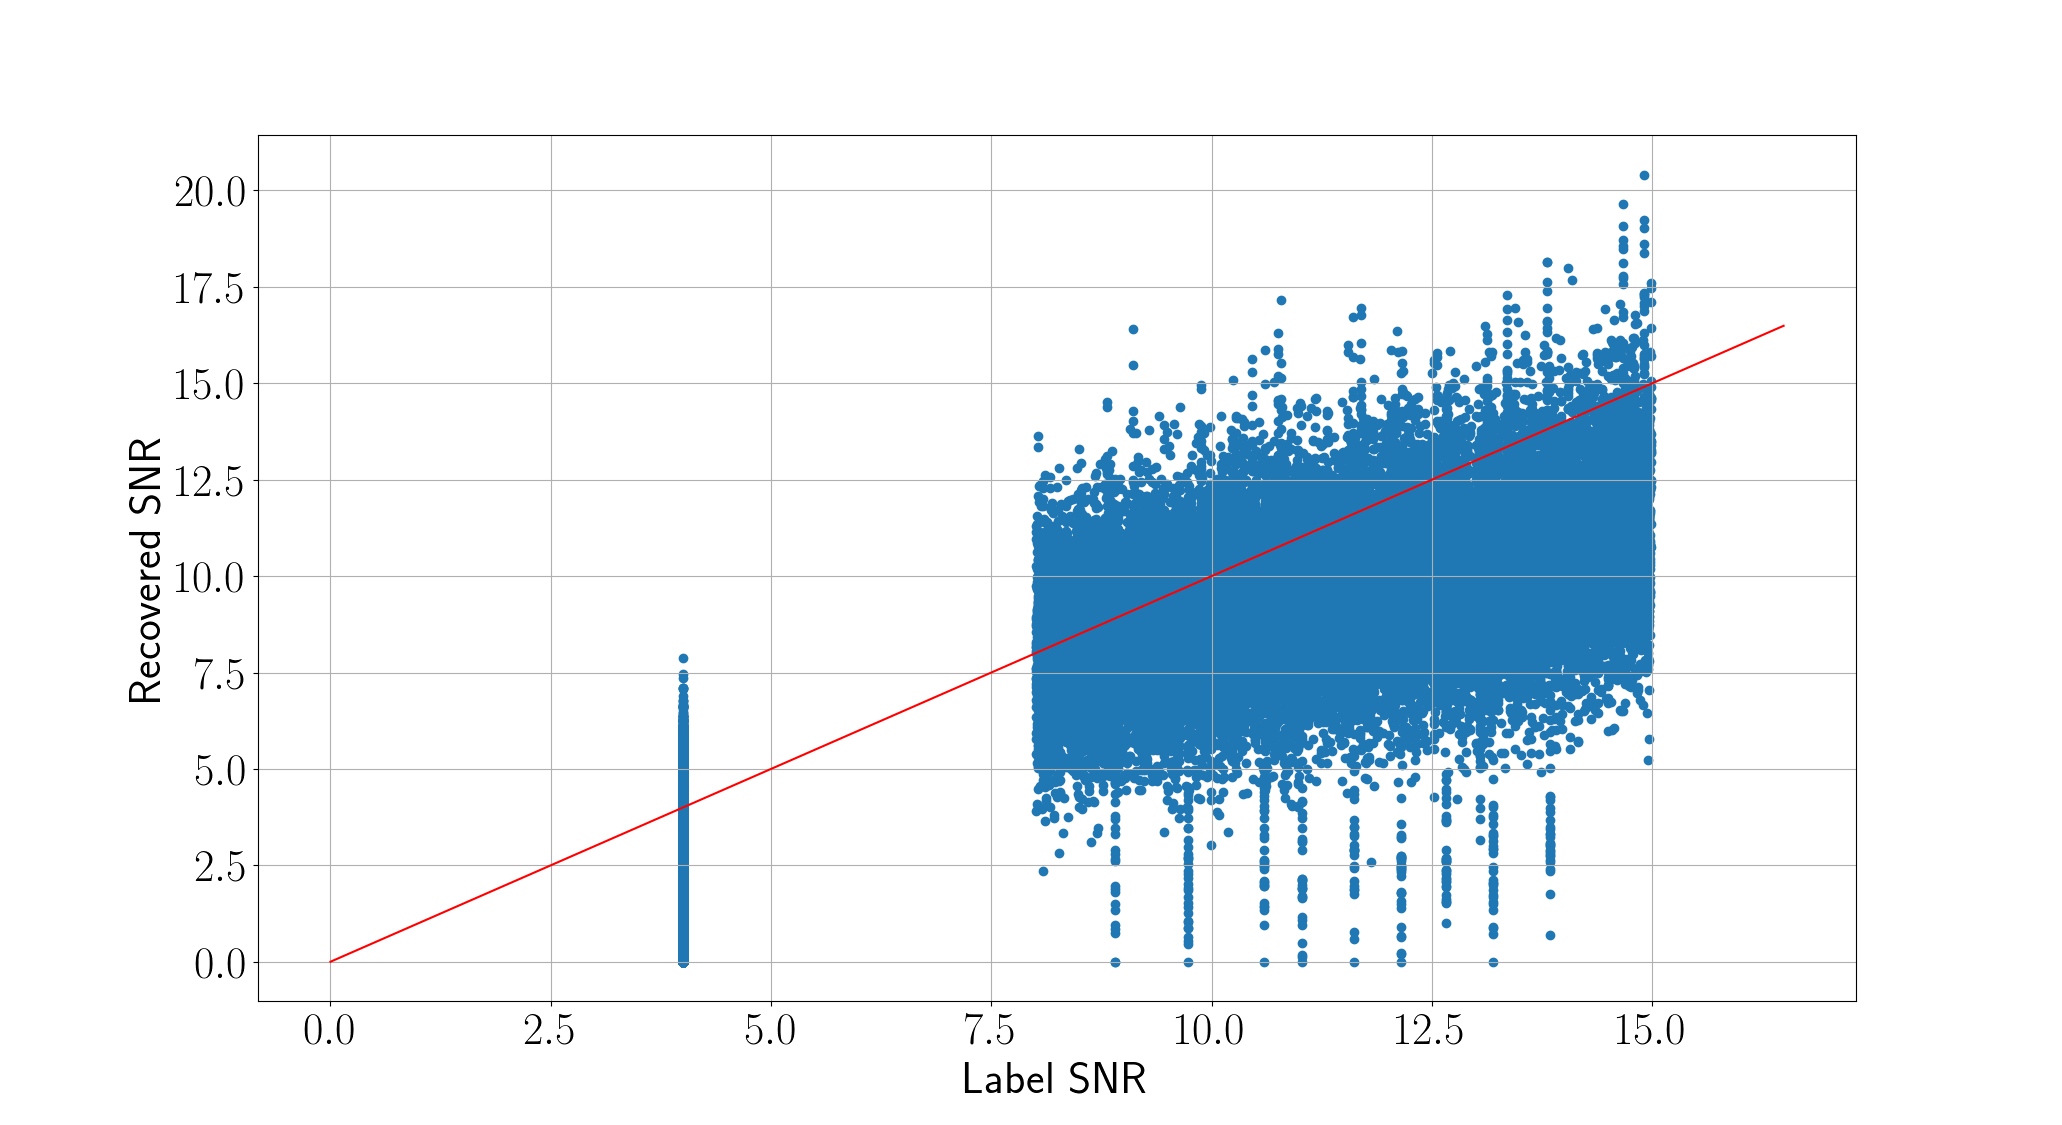
\includegraphics[width=0.75\textwidth]{streak_plot.png}
\caption[Plot of recovered values showcasing an error]{Shown are the recovered \gls{snr} values on the y-axis and the label values on the x-axis. Each \gls{snr} label has multiple y-values assigned to it, as the same waveform is submerged in multiple different noise realizations. The red line indicates where the dots should lie if the network recovered them without error. The dots roughly follow this line with the exception of a few streaks going down to 0. These are the waveforms that resonate strongly with the signal that was mistakenly added to every pure noise sample. Later iterations of the architecture reduced the number of streaks down to a single one.}\label{fig:streak_plot}
\end{figure}
The observed behavior and the incredible performance was due to a bug in how the network was fed with data. The generator combines a pure waveform with one noise realization to create a signal sample and is supposed to combine an array of zeros with a noise realization for a pure noise sample. A missing ''if''-statement led to the array of zeros always being replaced with the waveform that was the last in the list of available waveforms. Therefore, instead of pure noise, the network always saw noise plus one specific waveform. The same error with the exact same waveform was present in both the training and the validation set which made this error hard to catch. In fact the error was only discovered about two weeks after it first occurred. Finding the bug this late led to the optimization of the architecture for this flawed data. The best performing network had a sensitivity of more than 95\% over the entire \gls{snr} range for this flawed data, even once we used more difficult data, i.e. varying more parameters than just the \gls{snr}.\\
Though this mistake might at first seem like a waste of time, it actually helped in two aspects. Firstly, it showed the possibility for a network to consistently recover a single sample from different noise realizations and being able to model it well enough. The hurdle for a general search isn't trivial from this point, as in an optimal case we would expect the network to generalize the structure of the waveforms it was trained on and interpolate a template bank, but it is a starting point. Secondly, the optimization led to architectures with improved performance over for instance the \gls{tcin}s, when evaluated on non-flawed data. For this reason, we will list a few of the notable improvement here.\smallskip\\
The first observation was that the mistake of using filter sizes $(1,2,3)$ was actually an improvement over using $(4,8,16)$, which was previously used and found to be beneficial.
% (see (27.06.2019 (2)) in \cite{network_wiki}).
 Another feature introduced was the reduced number of input samples. Before the different sample rates had some overlap in the time domain, i.e. the last second of the data was sampled by all 7 rates, the last 2 seconds were sampled by all but the highest sample rate and so on. As the higher sample rates also contain all the information the lower sample rates do, this overlap was thrown away. For a detailed description of how this non overlapping multi-rate sampling works see \autoref{sec:data_generating_process}. A study, testing the two different approaches to sampling the data and reducing the number of input samples by simply using less sample rates, showed that using all sample rates is beneficial, while cropping the overlapping part of the data has no considerable negative effect.\\
 % (see 02.07.2019 (2) and following in \cite{network_wiki})\\
With the performance these architectures suggested, we moved to more difficult data, altering not only the \gls{snr} but also component masses $m_1, m_2$, coalescence phase $\Phi_0$, sky-position $\theta, \varphi$ and inclination $\iota$. As expected, the performance decreased a bit using more difficult data. Trying to recover the old performance led to one of the final improvements to the architecture. Instead of using a single inception stack, we introduced an architecture that is a mixture of the collect-inception networks and the pure inception networks. It uses the same inputs as the collect-inception networks, but cascades down concatenating two stacks after two inception layers, reducing the initial 8 stacks to 4. These 4 stacks each are fed through two further inception layers before being concatenated again. This procedure is repeated a third time, which results in a single stack of inception layers which is than fed to dense layers, in order to get the outputs. See \autoref{fig:cascade_inception_res_net} for an overview of the architecture. We will still refer to networks with a similar structure as collect-inception-res networks.\\
It again improved results a by a little. The sensitivity now didn't drop below 97\% for any of the bins, with the loudest noise sample having an \gls{snr} $\sim 8$. This is the last and best performing iteration of the network we found before the bug in the generating process was discovered and fixed. It therefore is still one of the core structures of the final architecture.\medskip\\
\begin{figure}
\centering
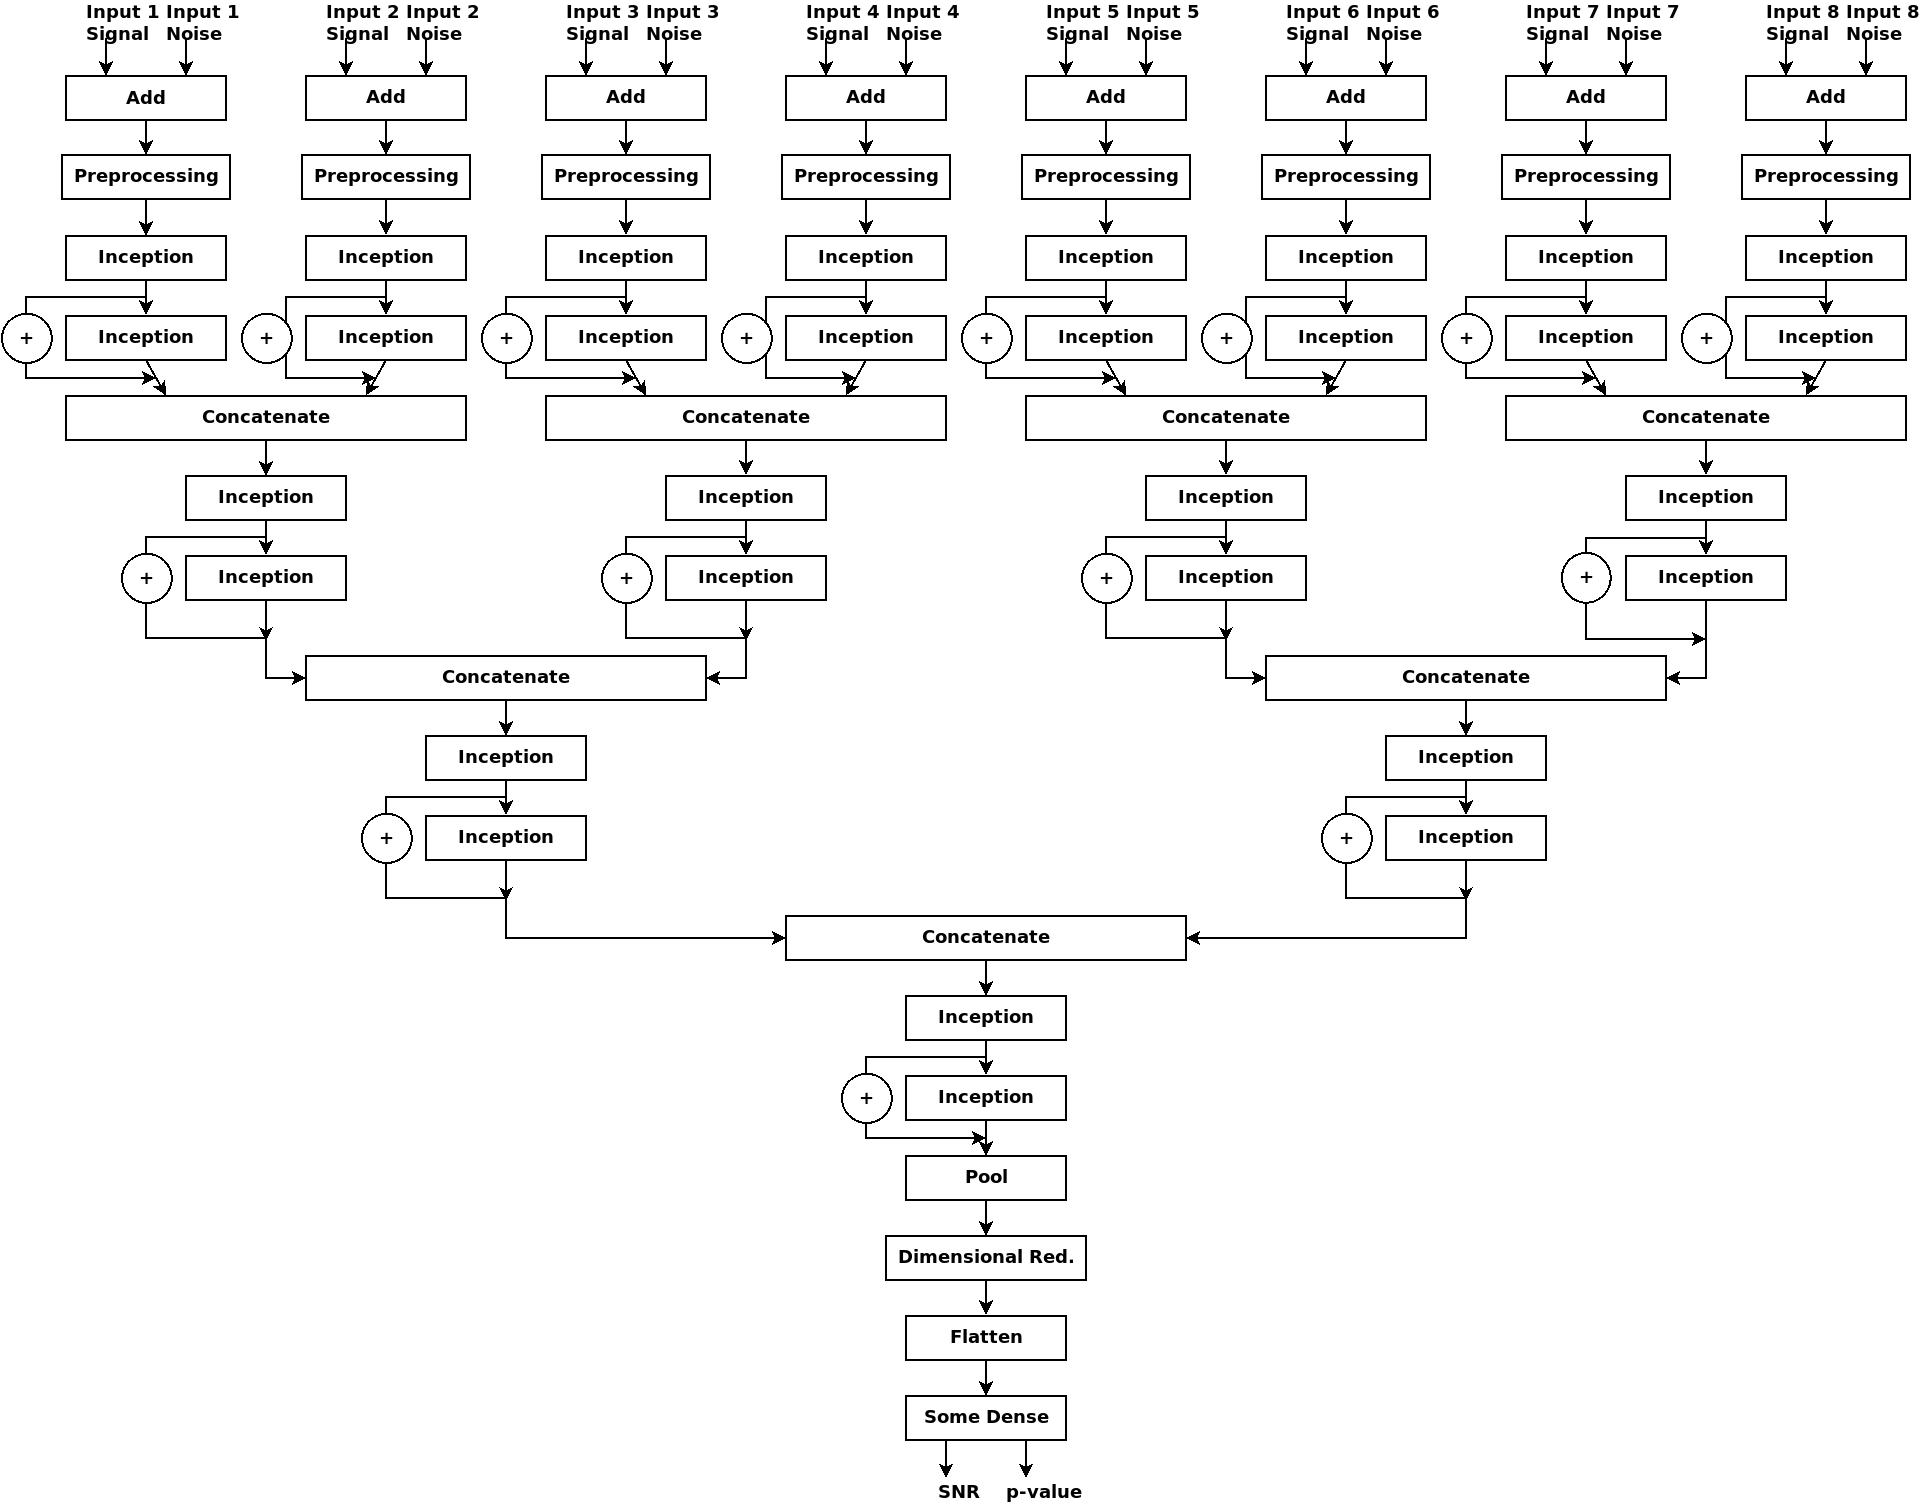
\includegraphics[width=\textwidth]{collect_inception_res_net_rev_1.png}
\caption[Cascading architecture of a collect-inception-res network]{The rough architecture of a cascading collect-inception-res network is shown. The preprocessing layers contain 2 convolutional layers as well as some dropout and batch normalization. The block labeled ''Some Dense'' actually consists of two separate stacks of dense layers, that reduce the output of the last inception layer down to the appropriate size. \textcolor{red}{Work on this graphic and make it a bit larger.}}\label{fig:cascade_inception_res_net}
\end{figure}

\noindent Using the corrected data generator with the previously well performing inception-res networks on data, where all previously mentioned parameters were being varied, showed how big the impact of the error was. The sensitivity dropped from 95\% in every \gls{snr} bin to below 20\% in the loudest bin. The collect-inception-res network held up a bit better, dropping to 40\% sensitivity in the loudest bin. From this point we tried to recover some of the lost performance by developing new features and implementing them into the collect-inception-res network.\medskip\\
One of the first tests was training the network to just optimize the p-score rather than both \gls{snr} and p-score, as this second output usually performed a little better than the \gls{snr} output. This did however not work and decreased the performance of the network significantly, reaching only $\sim 12\%$ at the loudest point. Using the original architecture with both outputs but adding in one more inception module per stack also resulted in worse performance overall. This decrease, however, was not quite as significant, dropping only to 30\% in the loudest bin.\smallskip\\
One of the prominent problems the network has is that estimating pure noise with a large \gls{snr} value significantly decreases sensitivity. An overestimated noise sample is a lot worse than an underestimated signal, as the former has an effect on all \gls{snr} bins. Therefore we tried to implement a loss function that mimics this behavior, by growing exponentially for overestimating noise and only linearly for underestimating it. For signals this behavior is mirrored, i.e. the loss grows exponentially for underestimating signals and linearly for overestimating them. The details on how this loss looks like and how it was derived can be found in \autoref{app:custom_loss}. It turned out that this approach also didn't help but rather decreased the sensitivity of the network. It even seemed to push the two categories closer together. Further research in this area might prove useful though.\medskip\\
% (see 21.07.2019 in \cite{network_wiki}). Other tests (e.g. (22.07.2019 (2)) in \cite{network_wiki}) showed similar results.\medskip\\
Another approach we took was close in nature to that of SincNet \cite{sincnet}. SincNet convolves the input data with a parameterized filter, that is used in standard signal processing. This has two main advantages. Firstly, the filters the network applies become more interpretable and thus reveal more insight into what the network is actually trying to accomplish. Secondly, the number of trainable parameters is reduced as we don't need to train a large convolution kernel but rather some parameters of a known function. Their implementation used the parametrized layer only as the first layer of the architecture and showed improvements over other purely convolutional approaches when trying to recognize speakers \cite{sincnet_speach}. Based on this work we used our adaptation only as a first layer, too. Instead of using Sinc-functions, we tried to use sums of sine waves. The convolution kernel is thus given by $\sum_{i=1}^n A_i\cdot\sin\lr{f_i t + \varphi_i}$, where $A_i$, $f_i$ and $\varphi_i$ are learned parameters and $t$ is used to sample the function. The general idea behind this approach is to enable the network to construct a crude template of a general waveform by combining multiple sine waves. To restrict the available frequencies, the layer is given a low and high frequency cutoff. This restriction is necessary to determine the shape of the convolution kernel. To sample a sine wave of frequency $f$, according to Nyquist, one needs to sample at least with a rate of $2f$. Therefore the sample rate is given by $\diff t = \frac{1}{2 f_\text{high}}$. As we want to fit at least one complete cycle of the lowest frequency into our kernel, the number of samples in the kernel is given by $N=\frac{f_\text{low}}{2f_\text{high}}$. By default the convolution kernel will always be filled with samples, e.g. a sine wave of frequency $f=2f_\text{low}$ will manage two full cycles in the convolution kernel. We called this layer ''Wave-Convolution'' or ''WConv1D'' in short and will from here on out refer to it by this name.\\
To get a quick estimate of how well this new approach does we devised a simple network consisting of only two convolution-type layers and two dense layers to get the correct output. We than compare two iterations of this network, one trained with the new Wave-Convolution layer and one using a usual convolutional layer. All other parameters are kept constant. For the convolutional layer, we choose the kernel size in such a way that the number of trainable parameters is on a comparable scale.\\
First tests of this new layer did apply some false windowing and used a skewed methodology. The results produced by these early tests lost out to pure convolutional quite strongly and thus this approach was not further pursued. Revisiting the idea close to finishing this project and fixing the errors previous runs made paints a different but not clear picture. Now the WConv1D layer significantly outperforms the traditional convolutional layer, almost doubling the sensitivity in every bin. The results are however questionable in multiple ways. Firstly, both networks experienced strong overfitting, thus rendering the training almost meaningless. Therefore, the difference in performance may be down to pure chance. Secondly, the networks were only followed by a single convolutional layer before being fed into the final dense layers. The test setup therefore doesn't consider the impact on deep networks. Furthermore, the convolution kernel used for the convolutional network was of size 288, which is well beyond the usual kernel sizes of 16 used in \gls{cnn}s designed for filtering \gls{gw} data. It is thus questionable if the extra effort required would justify the use of a WConv1D layer. Finally, the layer was not compared in state of the art networks derived above. Therefore, a lot more research would be necessary to determine the use of this new approach.\medskip\\
As no architectural alteration proved to be highly beneficial to the performance of the network for the difficult data where a lot of parameters are varied, we went back to using the data that only varies the \gls{snr}. We than combined the general approach of the \gls{tcin} with the new cascading architecture and found that it outperforms the traditional \gls{tcin}. This combination is the final architecture we tried and will be explained in further detail in \autoref{sec:final_architecture}. We then used this final architecture and trained it on the data described in \autoref{sec:data_generating_process} to finally evaluate it.\medskip\\
We conclude this section with a few statements about general findings of our research.\\
Using dropout layers in the initial layers after normalizing the input generally had a positive effect on the achievable sensitivities, even when the number of input samples was chosen large enough to avoid overfitting. It generally however comes with the disadvantage of the loss being a lot more jumpy throughout the training and trends in the loss being washed out.\\
We used the \gls{sgd} variant ''Adam'' as an optimizer for most of our runs and did not see improvements when trying different ones like ''AdaDelta'' or standard \gls{sgd}. We also briefly tried modifying the learning rate but could not improve results, thus staying with the default learning rate of $10^{-3}$.\\
Finally, when training a network and monitoring the sensitivity throughout the training process, we noticed drops to zero sensitivity at some point. These got more frequent as training went on. We hypothesize that this drop is due to the network trying to split noise and signals rather strongly. If one of the noise samples resonates strongly with the network and it ''thinks'' to have seen a signal, it will push the value for this sample higher and higher. The p-score additionally will saturate at 1. We therefore recommend to stop training the network after a few of these dips to 0 sensitivity occurred.


\subsection{Final Network}
\textcolor{blue}{Talk about how the final network looks, how it performs and what could be imporved.}\\
\textcolor{red}{First final network stored at tcn\_collect\_inception\_res\_net\_rev\_6\_248201905643}\\
Trying to optimize a \gls{nn} to a specific task is a problem that has no specified end. Therefore, the architecture discussed in this section is only the best of our current efforts. We will start off by discussing it and the underlying design decisions in detail and afterwards evaluate the performance on a long set of continuous strain data.
\subsubsection{Architecture}\label{sec:final_architecture}
\textcolor{blue}{Explain the architecture and the reasoning behind it. Talk about the size of the model, where it could be trained and what the drawbacks of the architecture are. (Drawbacks: Large memory size (hence small batch size), very deep $\to$ slow training and maybe vanishing gradients, hyper-parameter-optimization is hard, not everywhere are residual connections (fixable by further dimensional reduction))}\\
All illustrations for this section can be found in \autoref{app:illustrations_final_architecture}.\\
The final architecture is a collect-inception-res network with \gls{tcn}s as denoisers for every stack. Each stack is attributed its own sample rate and they cascade down to the two outputs. The first output is supposed to give an estimate of the \gls{snr} of the input data whereas the second one gives a p-score, a value that is used for pure binary classification, i.e. just gives information about whether or not a \gls{gw} is present in the data. To stress again, the p-score is not a probability but just a value that is bounded by 0 and 1 that, when a threshold is applied, gives a binary answer. A high-level overview of the network is shown in \autoref{fig:high_level_final_network}.\\
We will now give a detailed description of each module depicted in \autoref{fig:high_level_final_network}, working our way down from the input. We will only discuss each module once, as all of them share the same parameters.\\
The inputs are labeled 1 to 8, each consisting of an individual input for signal and noise. The order of these inputs is the reversed order of the chopped up time series, i.e. input 1 corresponds to the last \SI{0.5}{\s} of data sampled at \SI{4096}{\hertz}, input 2 is the interval from \SIrange{0.5}{1}{\s} sampled at \SI{4096}{\hertz} and so on. The final input thus is the last \SI{32}{\s} sampled at \SI{64}{\hertz} (for details see \autoref{sec:data_generating_process}). The first layer in each stack simply adds the two stack-inputs for signal and noise together. This sum is then fed to a \gls{tcn}.\\
The \gls{tcn} stacks 11 blocks of dilated convolutional layers with causal connections on top of each other. Every block has a total kernel size of three and the dilation is set to $2^i$, where $i$ is the depth of the \gls{tcn}. Furthermore, each block consists of two stacked convolutional layers with dilation rate $2^i$, each followed by a  batch normalization, ReLU activation and dropout layer. The latter has a dropout rate of 0.1. Finally, the entire block is preceeded by a dimensional reduction layer and wrapped with a residual connection. (see \autoref{fig:tcn_block}) The implementation follows \cite{tcn_paper}, replacing their weight normalization by batch normalization, as Keras does not provide a weight normalization layer. The depth was chosen such that the receptive field of the \gls{tcn} encapsulates all $2048$ input samples.\\
Each of the \gls{tcn} has their own training goal, which is given by the corresponding signal input. The loss for this part is chosen to be \gls{mse} and added to the total loss with a weight factor of $0.1$. The weight is set so low as the \gls{tcn} is not able to reliably recover the waveform from the input data and we don't want the network to try and optimize just the \gls{tcn}s without optimizing the final outputs we care about. With this training goal, the \gls{tcn} is meant to act as a denoiser to the input data. Its output is then added back onto the input, to amplify any signal it found. To avoid throwing away information the \gls{tcn} could not recover, we only amplify the signal and don't just feed the output itself to the following layers.\\
As a next step we do some preprocessing for the following collect-inception-res network. The authors of \cite{inception_module} found that using a few simple convolutional layers before a stack of inception modules helps the network learn. We could verify these findings when testing different inception networks and thus included this preprocessing step. It starts of with a batch normalization layer, followed by a dropout layer with a dropout rate of $0.25$. They are followed by two stacked blocks of convolution, batch normalization and ReLU activation, separated by a max pooling layer with pool size 4. See \autoref{fig:preprocessing} for a visual aid.\\
The main workhorse for the collect-inception-res network are the inception blocks. Each of them contain two stacked inception modules, separated by a batch normalization layer. The second inception module also utilizes a residual connection. The first one could be equipped with a residual connection as well if it was preceded by a  dimensional reduction layer, adjusting the number of channels to $224$. Within the inception modules, we empirically chose the number of filters to be descending for an increasing kernel size. We furthermore found that kernel sizes $(1,2,3)$ work best in these modules. These parameters could probably be optimized even further, but we could not do so in a feasible amount of time. The inception block is depicted in \autoref{fig:inception_block}.\\
All concatenation layers except the final one are furthermore equipped with another auxiliary output that use the \gls{snr} label as a training goal. To reduce each of these layers down to a single value we use a stack of one average pooling layer with pool size 8, one dimensional reduction layer with 16 filters and one final dense layer with a single neuron and a ReLU activation function. The output of the dimensional reduction is flattened to be usable for a dense layer. This action was taken to help against vanishing gradients and was inspired by the architecture of \cite{inception_module}. The loss used is \gls{mse} and is also weighted by $0.1$.\\
The post-processing consists of a max pooling layer with pool size 4, a dimensional reduction layer with 32 filters and, depending on the output, two dense layers with neuron numbers $(2,1)$ for the \gls{snr} output and $(3,2)$ for the p-score output. For the \gls{snr} output we use a ReLU activation function and for the p-score output a softmax activation function. The loss for the \gls{snr} output is \gls{mse} and has a weight of $1$ whereas the p-score output uses a categorical crossentropy as loss and a weight of $0.5$ to have more of an emphasis on the \gls{snr}. The postprocessing step is shown in detail in \autoref{fig:postprocessing}.\medskip\\
This architecture was derived empirically by the process described in \autoref{sec:evolution_of_architecture} as it showed the best performance in regards to the sensitivity on the validation set. The specifics of the performance are discussed in the next section. It does, however, come with multiple drawbacks. The general problem of this architecture is its size and complicated structure. The first obvious complication is the size of necessary video memory. The model takes about \SI{18}{\giga\byte} to train with a mini-batch size of 24. The GPU with the largest memory we could use for a full training run was a NVIDIA Titan V with a capacity \SI{\sim 12}{\giga\byte}. To train this network on such limited memory required us to decrease the mini-batch size to 16. Even though the network just barely fit into memory and Tensorflow stated that additional performance might be gained if more memory was available. This is backed by the GPU utilization that constantly jumped between 20\% and 100\%. Overall each epoch training on the stated $322,500$ sample plus the validation step took \SI{\sim 6}{\hour} to finish.\\
As each epoch takes such a long time, it is very difficult to optimize the hyper parameters, like number of inception modules, kernel sizes within these modules, number of filters in these modules, dropout rate, etc.\\
Finally, a network of this depth is always vulnerable to the vanishing gradient problem. We try to combat this with the auxiliary outputs and their loss functions but cannot rule it out.

\subsubsection{Network Performance}\label{sec:network_performance}
\textcolor{blue}{Evaluate the performance of the network. Show sensitivity curves, talk about speed advantages, how does it in both cases compare to matched filtering? How does it compare to related works? (Reference the BNS-Net paper, what is different between our approach and theirs? Why does theirs seem to work a lot better? Does it?)}
%\textcolor{blue}{Compare the speeds of both methods, the accuracy. What kind of drawbacks does the network have, what are its advantages, how should it be used and understood? (Not as a standalone method of analysis but rather as a starting point for samplers and a quick way of estimate certain properties.)}


\section{Conclusions}
\begin{comment}
\textcolor{blue}{Well duh, give a conclusion and maybe outlook.}\\
\textcolor{red}{Mention that the PyCBC Live pipeline has probably (talk to Alex about this) a higher latency than our search (they have latency on average \SI{16}{\s} \cite{pycbc_live}) but already give rough parameter estimation and sky localization which we can't do. They furthermore are a lot more sensitive.}
\begin{itemize}
	\item First time anybody tested sensitivity of a \gls{nn} for \gls{bns} signals at such a low false alarm rate
	\item Computationally very efficient therefore lower latency (need to quantify this)
	\item At the moment network probably too complicated and therefore hyper parameters probably not optimal
	\item Introduced new architecture of using a TCN as denoiser. Also the cascading architecture is new and promising
	\item Network not yet ready to use
	\item Couldn't work with real detector data yet, as it also wouldn't be sensible with our sensitivity
	\item Still interesting as it has shown potential with easier data
\end{itemize}
\end{comment}
This work has explored a completely new set of architectures in their application to \gls{gw} data analysis. We introduced the concept of using multiple sample rates to reduce the number of input samples to the network and thus decrease the size of the network, while retaining a lot of the information of the long signals that are emitted by \gls{bns} systems. Testing multiple different architectures led to the use of inception modules and the \gls{tcn}s as amplifiers for the input signal. Our design process led to a very deep and wide architecture utilizing multiple techniques pioneered for image recognition tasks. To the best of our knowledge we are also the first to use the \gls{snr} as a training goal, thus providing a direct ranking statistic for every event.\\
We have for the first time tested the sensitivity of a \gls{nn}-based search at very low false alarm rates for \gls{bns} signals. The final architecture suggests that it might be possible to reach meaningful false alarm rates that are low enough to alert astronomers of possible \gls{gw} events. Though we have not managed to fully reach the goal of acceptable sensitivities at a false alarm rate of \SI[per-mode=fraction]{1}{\sample\per\month}, our network significantly improves upon previously tested architectures.\\
We do, however, find that a search pipeline using our \gls{nn} to detect \gls{bns} signals is not yet sensible. Current matched filter pipelines are superior in every aspect. Not only are they more sensitive to the signals we used to train our network, but are also computationally more efficient, which was the main reason to explore machine learning search pipelines. The gap in efficiency is mostly down to the high complexity of the final architecture. We furthermore did not test the sensitivity of the network on real detector data which contains non Gaussian noise transients and can thus not claim any implications for a real search.\\
Using the \gls{snr} as training goal has proven to be a difficult problem. Using it to generate detection candidates yields slightly worse sensitivities at low false alarm rates. At high false alarm rates this difference vanishes. We did, however, find that this output is a lot more fragile and can produce realistic detection values for unrelated data. The p-score is a lot more resilient to such inputs and can also be interpreted as a ranking statistic, rather than a binary output.\\
We hope that our work, although not yielding a useful search pipeline will prove useful to the field of utilizing machine learning algorithm to detect \gls{gw}s. This thesis has tested multiple new approaches to the architecture and has found great improvements over the current state of the art convolutional architectures, by deploying inception modules. We have furthermore given an overview of a process which we believe produces reliable estimates of false alarm rates and sensitivities by sliding our network across a continuous input.\smallskip\\
As a next step we would like to improve the complexity of our architecture while retaining its sensitivity. Doing so would yield better computational efficiency and enable us to do more efficient hyper parameter exploration, which in turn will hopefully improve the performance even further. We will also test different formats for the input data, as others have used shorter parts but sampled at a higher rate. Finally, as a long term goal, we would like to incorporate and test real detector data and turn this approach into an independent search pipeline. To give security against data that accidentally resonates strongly with the network this pipeline should be backed up by a matched filter pipeline that only covers a small parameter space.


\section{Acknowledgments}
\textcolor{red}{Acknowledge Frank, Alex, Christoph, AEI, spell and grammar checkers.}

\appendix

\section{Full Adder as Network}\label{app:Full_adder}
To create a full adder from basic neurons, the corresponding logic gates need to be defined. The equivalent neuron for an ''and''-gate was defined in \autoref{sec:basics_neuron_network}. There are two more basic neurons which will be defined here. The neuron corresponding to the ''or''-gate, which is given by the same activation function \eqref{def:step_activation}, weights $\vec{w}={(w_1, w_2)}^T=(1,1)$ and bias $b=-0.5$, and the neuron equivalent to the ''not''-gate, which is given by the activation function \eqref{def:step_activation}, weight $w=-1$ and bias $b=0.5$. These definitions are summarized in \autoref{tab:neuron_logic_gates}.
\begin{table}[H]
\begin{center}
\begin{tabular}{c|c|c}
''and''-neuron & ''or''-neuron & ''not''-neuron\\
\hline
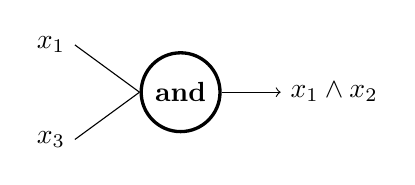
\begin{tikzpicture}[
neuron/.style={circle, draw=black, very thick, minimum size=1.0cm},
dot/.style={circle, draw=black, fill=black, minimum size=0.1cm, inner sep=0pt},
VLineVertex/.style={circle, draw=black, minimum size=0cm, inner sep=0pt},
]

\node[neuron] (neuron) {\textbf{and}};
\node (place) [left=1cm of neuron] {};
\node (x1) [above=0.25cm of place] {$x_1$};
\node (x3) [below=0.25cm of place] {$x_3$};
\node (out) [right=0.75cm of neuron] {$x_1\land x_2$};

\draw (x1.east) -- (neuron.west);
\draw (x3.east) -- (neuron.west);
\draw [->] (neuron.east) -- (out.west);

\end{tikzpicture} & 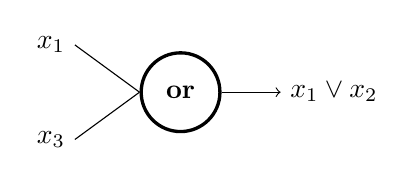
\begin{tikzpicture}[
neuron/.style={circle, draw=black, very thick, minimum size=1.0cm},
dot/.style={circle, draw=black, fill=black, minimum size=0.1cm, inner sep=0pt},
VLineVertex/.style={circle, draw=black, minimum size=0cm, inner sep=0pt},
]

\node[neuron] (neuron) {\textbf{or}};
\node (place) [left=1cm of neuron] {};
\node (x1) [above=0.25cm of place] {$x_1$};
\node (x3) [below=0.25cm of place] {$x_3$};
\node (out) [right=0.75cm of neuron] {$x_1\lor x_2$};

\draw (x1.east) -- (neuron.west);
\draw (x3.east) -- (neuron.west);
\draw [->] (neuron.east) -- (out.west);

\end{tikzpicture} & 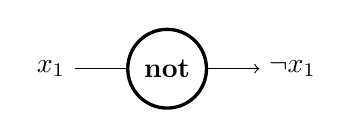
\begin{tikzpicture}[
neuron/.style={circle, draw=black, very thick, minimum size=1.0cm},
dot/.style={circle, draw=black, fill=black, minimum size=0.1cm, inner sep=0pt},
VLineVertex/.style={circle, draw=black, minimum size=0cm, inner sep=0pt},
]

\node[neuron] (neuron) {\textbf{not}};
\node (x1) [left=0.65cm of neuron] {$x_1$};
\node (out) [right=0.65cm of neuron] {$\lnot x_1$};

\draw (x1.east) -- (neuron.west);
\draw [->] (neuron.east) -- (out.west);

\end{tikzpicture}\\
\hline
\begin{tabular}{c c}
$\vec{w}=(1,1)$ & $b=-1.5$
\end{tabular} &
\begin{tabular}{c c}
$\vec{w}=(1,1)$ & $b=-0.5$
\end{tabular} &
\begin{tabular}{c c}
$w=-1$ & $b=0.5$
\end{tabular}\\
\hline
\begin{tabular}{c c|c}
$x_1$ & $x_2$ & $a(x_1+x_2-1.5)$\\
\hline
$0$ & $0$ & $0$\\
$0$ & $1$ & $0$\\
$1$ & $0$ & $0$\\
$1$ & $1$ & $1$\\
\end{tabular} &
\begin{tabular}{c c|c}
$x_1$ & $x_2$ & $a(x_1+x_2-0.5)$\\
\hline
$0$ & $0$ & $0$\\
$0$ & $1$ & $1$\\
$1$ & $0$ & $1$\\
$1$ & $1$ & $1$\\
\end{tabular} &
\begin{tabular}{c|c}
$x_1$ & $a(-x_1+0.5)$\\
\hline
$0$ & $1$\\
$1$ & $0$\\
\end{tabular}
\end{tabular}
\end{center}
\caption[Logic gates as neurons]{A summary and depiction of the main logic gates written as neurons. All of them share the same activation function \eqref{def:step_activation}.}\label{tab:neuron_logic_gates}
\end{table}
\medskip
\noindent Using the basic logic gates a more complex structure - the ''XOR''-gate - can be built. A ''XOR''-gate is defined by its truth table (see \autoref{tab:xor}).
\begin{table}[H]
\centering
\begin{tabular}{c c|c}
$x_1$ & $x_2$ & $x_1\veebar x_2$\\
\hline
$0$ & $0$ & $0$\\
$0$ & $1$ & $1$\\
$1$ & $0$ & $1$\\
$1$ & $1$ & $0$
\end{tabular}
\caption[Truth table for  the ''XOR''-gate]{Truth table for the ''XOR''-gate.}\label{tab:xor}
\end{table}
It can be constructed from the three basic logic operations ''and'', ''or'' and ''not''
\begin{equation}
x_1\veebar x_2 = \lnot\lr{\lr{x_1\land x_2}\lor\lnot\lr{x_1\lor x_2}}.
\end{equation}
Therefore, the basic neurons from \autoref{tab:neuron_logic_gates} can be combined to create a ''XOR''-network (see \autoref{fig:xor_net}).\\
To simplify readability from here on out a neuron called ''XOR'' will be used. It is defined by the network of \autoref{fig:xor_net} and has to be replaced by it, whenever it is used.\\
With this ''XOR''-neuron a network, that behaves like a full-adder, can be defined. A full-adder is a binary adder with carry in and carry out, as seen in \autoref{fig:full_adder}.
\begin{figure}[H]
\centering
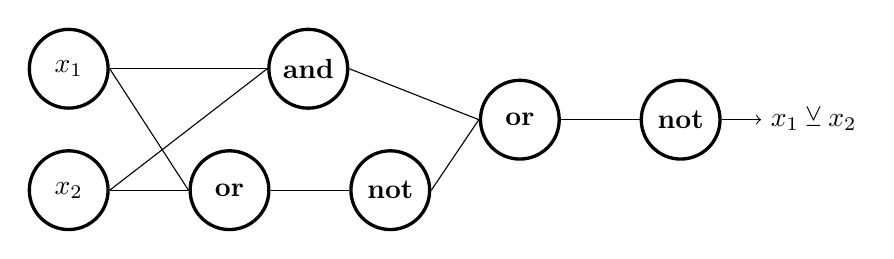
\begin{tikzpicture}[
neuron/.style={circle, draw=black, very thick, minimum size=1.0cm},
dot/.style={circle, draw=black, fill=black, minimum size=0.1cm, inner sep=0pt},
VLineVertex/.style={circle, draw=black, minimum size=0cm, inner sep=0pt},
]

\node[neuron] (out_not) {\textbf{not}};
\node[neuron] (final_or) [left=1cm of out_not] {\textbf{or}};
\node (between) [left=1cm of final_or] {};
\node[neuron] (bot_not) [below=0.25cm of between] {\textbf{not}};
\node[neuron] (bot_or) [left=1cm of bot_not] {\textbf{or}};
\node[neuron] (x2) [left=1cm of bot_or] {$x_2$};
\node[neuron] (x1) [above=0.5cm of x2] {$x_1$};
\node[neuron] (top_and) [right=2cm of x1] {\textbf{and}};
\node (out) [right=0.5cm of out_not] {$x_1\veebar x_2$};

%Input
\draw (x1.east) -- (top_and.west);
\draw (x2.east) -- (top_and.west);
\draw (x1.east) -- (bot_or.west);
\draw (x2.east) -- (bot_or.west);

%First and second layer connections
\draw (top_and.east) -- (final_or.west);
\draw (bot_or.east) -- (bot_not.west);
\draw (bot_not.east) -- (final_or.west);

%Final connection
\draw (final_or.east) -- (out_not.west);

%Output
\draw [->] (out_not.east) -- (out.west);
\end{tikzpicture}
\caption[''XOR''-network]{The definition of a network that is equivalent to an ''XOR''-gate.}\label{fig:xor_net}
\end{figure}
\begin{figure}[H]
\centering
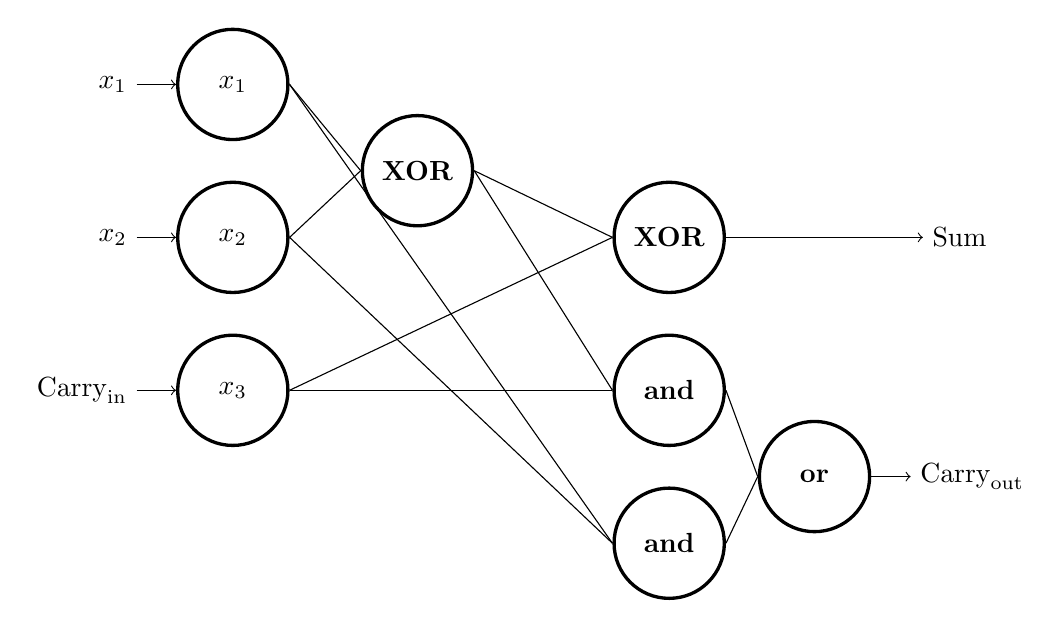
\begin{tikzpicture}[
neuron/.style={circle, draw=black, very thick, minimum size=1.4cm},
dot/.style={circle, draw=black, fill=black, minimum size=0.1cm, inner sep=0pt},
VLineVertex/.style={circle, draw=black, minimum size=0cm, inner sep=0pt},
]

\node[neuron] (x1) {$x_1$};
\node[neuron] (x2) [below=0.5cm of x1] {$x_2$};
\node[neuron] (x3) [below=0.5cm of x2] {$x_3$};
\node (center_xor1) [below=0.25cm of x1] {};
\node[neuron] (xor1) [right=1.5cm of center_xor1] {\textbf{XOR}};
\node[neuron] (xor2) [right=4.1cm of x2] {\textbf{XOR}};
\node[neuron] (and1) [below=0.5cm of xor2] {\textbf{and}};
\node[neuron] (and2) [below=0.5cm of and1] {\textbf{and}};
\node (center_or1) [below=0.25cm of and1] {};
\node[neuron] (or1) [right=1cm of center_or1] {\textbf{or}};
\node (out_sum) [right=2.5cm of xor2] {Sum};
\node (out_car) [right=0.5cm of or1] {$\text{Carry}_\text{out}$};

%Inputs
\node (x1_in) [left=0.5cm of x1] {$x_1$};
\node (x2_in) [left=0.5cm of x2] {$x_2$};
\node (car_in) [left=0.5cm of x3] {$\text{Carry}_\text{in}$};

%Draw lines
%Input arrows
\draw[->] (x1_in.east) -- (x1.west);
\draw[->] (x2_in.east) -- (x2.west);
\draw[->] (car_in.east) -- (x3.west);

%Input connections
\draw (x1.east) -- (xor1.west);
\draw (x1.east) -- (and2.west);
\draw (x2.east) -- (xor1.west);
\draw (x2.east) -- (and2.west);
\draw (x3.east) -- (xor2.west);
\draw (x3.east) -- (and1.west);

%xor1 connections
\draw (xor1.east) -- (xor2.west);
\draw (xor1.east) -- (and1.west);

%Third layer connections
\draw[->] (xor2.east) -- (out_sum.west);
\draw (and1.east) -- (or1.west);
\draw (and2.east) -- (or1.west);

%Or out
\draw[->] (or1.east) -- (out_car.west);
\end{tikzpicture}
\caption[Full adder network]{A network replicating the behavior of a binary full adder.}\label{fig:full_adder}
\end{figure}
\newpage

\begin{comment}
\section{Indication of a Local Minimum}\label{app:network_does_not_learn}
Sometimes during training only a local minimum is found. The most notable of these minima is when the network just picks a fixed value in the interval and appoints it to any input. It is therefore useful to spot this behavior during training and consider restarting. Therefore the value for a constant output will be calculated in this appendix.
\medskip\\
To start off the loss function will be assumed to be the mean squared error. Furthermore it is assumed, that the \gls{snr}-values lie within the interval $\left[a,b\right]$. The mean squared error of a chosen point $x$ to every point in this interval is given by
\begin{equation}
f(x)\coloneqq\frac{1}{b-a}\int_a^b\diff y\ \lr{x-y}^2=\frac{1}{3\lr{b-a}}\lr{\lr{b-x}^3-\lr{a-x}^3}.
\end{equation}
To minimize this one could in principle solve $\frac{\partial f}{\partial x}\mbe 0$ and it would yield the correct result. However it should at least intuitively be obvious that the point that minimizes the mean squared error to every point in the interval is the mean value of the interval $x=\frac{a+b}{2}$.\\
Therefore if the network has to choose values out of a given interval $\left[a,b\right]$, minimize the mean squared error and the training finds a local minimum that leads to the network always returning a fixed value, this value should be
\begin{equation}
f\lr{\frac{a+b}{2}}=\frac{1}{3\lr{b-a}}\lr{\lr{\frac{b-a}{2}}^3-\lr{\frac{a-b}{2}}^3}=\frac{1}{12}\lr{b-a}^2.
\end{equation}
In this work another common case is the network having to choose a \gls{snr}-value from some continues interval $\left[a,b\right]$ or pick a discrete value $c$. The interval corresponds to the data containing some \gls{gw}-signal and the fixed point with value $c$ is the \gls{snr}-value assigned to pure noise during training. (The following is by no means a strictly mathematical derivation but simply a quick way to calculate the expected value.) The mean squared error is hence given by
\begin{align}
g(x) & \coloneqq\lim_{n\to\infty}\lr{\frac{1}{n}\sum_{i=1}^{n}\lr{x-y_i}^2}\text{ with }
\begin{cases}
	y_i=a_i\in\left[a,b\right]\text{, probability }p\\
	y_i=c\text{, probability }(1-p)
\end{cases}\nonumber\\
& = \lim_{n\to\infty}\lr{\frac{1}{n}\sum_{i=1}^{p\cdot n}\lr{x-a_i}^2}+\lim_{n\to\infty}\lr{\frac{1}{n}\sum_{i=1}^{(1-p)\cdot n}\lr{x-c}^2}\nonumber\\
& = \lim_{n\to\infty}\lr{\frac{1}{n}\sum_{i=1}^{p\cdot n}\lr{x-a_i}^2}+\lim_{n\to\infty}\lr{\frac{(1-p)\cdot n}{n}\lr{x-c}^2}\nonumber\\
& \overset{(\ast)}{=} \lim_{n\to\infty}\lr{\frac{p}{n}\sum_{i=1}^{n}\lr{x-a_i}^2}+(1-p)\lr{x-c}^2\nonumber\\
& = p\underbrace{\lim_{n\to\infty}\lr{\frac{1}{n}\sum_{i=1}^{n}\lr{x-a_i}^2}}_{=f(x)}+(1-p)\lr{x-c}^2\nonumber\\
& = p f(x) + (1-p)\lr{x-c}^2,
\end{align}
where the step in $(\ast)$ is not trivial and would need a mathematical proof, but intuitively should be clear. \textcolor{red}{(If there is time, find a proof.)} For large $n$ all $a_i$ should contribute equally to the mean value and hence $p$ is just a proportionality factor.\\
With $\partial_x f(x)=2x-a-b$ one gets
\begin{equation}
\partial_x g(x) \mbe 0 \Leftrightarrow x = \frac{p}{2}\lr{a+b}+\lr{1-p}c
\end{equation}
as expected. The value of $g$ at this point will be the expectation value of the mean squared error if the network predicts a single value and optimizes this value. In this work $p$ is the probability of looking at data containing a \gls{gw}, i.e. the fraction of data-points containing a \gls{gw} over the total number of data-points.
\end{comment}

\section{Deriving Custom Loss}\label{app:custom_loss}
For this work the binary decision of ''signal'' vs. ''no-signal'' is more important for the performance of the network, than how accurate the predicted \gls{snr}-value is. Therefore, we would like the network to have a bias towards underestimating the \gls{snr}-values of pure noise examples and overestimate those of \gls{gw}-signals. To achieve this behavior, we tried to use a new loss function, that exponentially penalizes overestimating pure noise samples and underestimating \gls{gw}-signals. For backpropagation to work properly, the loss will need to be differentiable and its derivative needs to be continuous everywhere.\\
As a starting point we will use the pure noise case first and adapt it to the full loss later on. We start at a distribution of values we want to achieve and later turn it into an error function. This distribution should exponentially decay for values larger than some fixed value and decay like $1/x$ for values smaller than this fixed value. The exponential part was inspired by the solution of the hydrogen atom, though the decay for this case goes like $x^2$. For this reason, we matched
\begin{align}
f_1(x) & = x^2 e^{-x}\\
f_2(x) & = \frac{1}{a-b\cdot x}
\end{align}
for $x=1$, which gave
\begin{equation}
f(x)\coloneqq
\begin{cases}
	x^2 e^{-x}, & x \geq 1\\
	\frac{1}{e}\frac{1}{2-x}, & x < 1
\end{cases}.
\end{equation}
This distribution has its maximum value $\frac{4}{e^2}$ at $x=2$. For convenience, we will use
\begin{equation}
\text{dist}(x)\coloneqq f(x+2)
\end{equation}
from here on out, as the maximum is now centered at $x=0$. To get an error function from this distribution, that grows exponentially for $x>0$ and has a value of $0$ for $x=0$, define
\begin{equation}
\text{Err}(x)\coloneqq \frac{4}{e^2 \text{dist}(x)} - 1.
\end{equation}
To define a loss, that can behave differently for different label values, the error needs to transform based on some measure. Specifically it will need to have some transition between exponential growth for large values of $x$ and exponential growth for small values of $x$. To achieve this behavior, we rotate the error-function $\text{Err}$ around the y-axis and project it onto the x-y-plane afterwards. Therefore we get
\begin{equation}\label{def:err_rotate}
\text{Err}_\text{rotate}(x,\varphi)\coloneqq \text{Err}\lr{x/\cos\lr{\varphi}}.
\end{equation}
For $\varphi\in\left[0,\pi\right]$ this function is defined everywhere but $\varphi=\frac{\pi}{2}$.\\
To get a loss as defined in \eqref{def:general_loss} from \eqref{def:err_rotate}, it needs to depend not only on the value the network returns but also on the label. Furthermore, the exponential behavior should be governed by the label value, as we want exponential growth for positive differences, when the label is small, and for negative differences, when the label is large. To achieve this, the rotation angle will be dictated by the label value.\\
Therefore we want a function $g$, that is $0$ for all label values smaller than some minimum $a$ and $\pi$ for all label values larger than some maximum value $b$. In between $a$ and $b$, the function needs to be a smooth. The parts will be matched in a way to assure $g\in C^1(\R)$. With this one can find
\begin{equation}
g(x,a,b)\coloneqq
\begin{cases}
0, & x < a\\
\pi, & x>b\\
\pi p\lr{\frac{x-a}{b-a}}
\end{cases},
\end{equation}
with
\begin{equation}
p(x)\coloneqq 3x^2-2x^3.
\end{equation}
In principle the loss for given values $a$ and $b$ could than be written as
\begin{equation}\label{def:loss_original}
L_\text{exp}\lr{y_\text{net}, y_\text{label}}=\text{Err}_\text{rotate}\lr{z, g(y_\text{label},a,b)},
\end{equation}
with $z=y_\text{net}-y_\text{label}$. There are however problems with this definition. First of all, the exponential part is smaller than the linear part for small values of $z$. This is especially true for values $\left| z\right| <2$. This is a problem, as the \gls{snr}-value assigned to pure noise and the smallest signal \gls{snr}-value are about $4$ apart. Therefore, there would be an overlapping region for pure noise and small \gls{snr} signals, that is favored by the loss.\\
To solve this issue one can simply introduce a squish factor $s$, which the input to the error is multiplied by
\begin{equation}\label{def:loss_squished}
L_\text{squish}\lr{y_\text{net}, y_\text{label}}\coloneqq \text{Err}_\text{rotate}\lr{s\cdot z, g(y_\text{label},a,b)}.
\end{equation}
This however introduces a new problem. With even a relatively small squish factor of $s=3$, the exponential grows very fast, which causes exploding gradients. To keep the gradients at bay, a cutoff is introduced to the function. To still have a non zero gradient, this cutoff is not flat, but is a linear function with a slope of $\pm s\frac{4}{e}$, which is the same slope as the linear part of \eqref{def:loss_squished}. To keep the entire loss of class $C^1$, the exponential part and the cutoff are connected by a spline polynomial. For this, we chose to start the spline polynomial at some value $k-1$ from the origin and have it connect to the linear part in a distance of $1$. We restrict $k>1$.\\
With
\begin{gather}
%u = \max\left[\text{Err}_\text{rotate}\lr{s\cdot z + k, g(y_\text{label},a,b)},\ \text{Err}_\text{rotate}\lr{s\cdot z + k - 1, g(y_\text{label},a,b)}\right]\nonumber\\
u = \text{Err}\lr{s\cdot k}\nonumber\\
%l = \min\left[\text{Err}_\text{rotate}\lr{s\cdot z + k, g(y_\text{label},a,b)},\ \text{Err}_\text{rotate}\lr{s\cdot z + k - 1, g(y_\text{label},a,b)}\right]\nonumber\\
l = \text{Err}\lr{s\cdot\lr{k-1}}\nonumber\\
\Delta_1 = \frac{4 s^2 (k-1)}{\lr{2+s\cdot (k-1)}^3}e^{s\cdot (k-1)}\nonumber\\
\Delta_2 = s\frac{4}{e}\nonumber\\
a_1 = \Delta_2 + \Delta_1 - 2\lr{u-l}\nonumber\\
a_2 = 3\lr{u-l} - 2\Delta_1 - \Delta_2
\end{gather}
and
\begin{equation}
p_2(z)\coloneqq a_1 \lr{z-k+1}^3 + a_2\lr{z-k+1}^2 + \Delta_1 \lr{z-k+1} + l
\end{equation}
one gets
\begin{equation}
L_\text{large}\lr{y_\text{net}, y_\text{label}}\coloneqq
\begin{cases}
	\text{Err}_\text{rotate}\lr{s\cdot z, g(y_\text{label},a,b)}, z>-k+1\\
	p_2\lr{-z}, z\in\left[-k, -k+1\right)\\
	s\frac{4}{e}\left|z\right|+\text{Err}_\text{rotate}\lr{-s\cdot k, g(y_\text{label},a,b)}-s\cdot k\frac{4}{e}, z<-k\\
\end{cases}
\end{equation}
and
\begin{equation}
L_\text{small}\lr{y_\text{net}, y_\text{label}}\coloneqq
\begin{cases}
	\text{Err}_\text{rotate}\lr{s\cdot z, g(y_\text{label},a,b)}, z<k-1\\
	p_2\lr{z}, z\in\left[k-1, k\right)\\
	s\frac{4}{e}\left|z\right|+\text{Err}_\text{rotate}\lr{s\cdot k, g(y_\text{label},a,b)}-s\cdot k\frac{4}{e}, z>k\\
\end{cases}.
\end{equation}
The complete loss is than given by
\begin{equation}
L_\text{full}\lr{y_\text{net}, y_\text{label}}=
\begin{cases}
L_\text{small}\lr{y_\text{net}, y_\text{label}}, y_\text{label}<\frac{a+b}{2}\\
L_\text{large}\lr{y_\text{net}, y_\text{label}}, y_\text{label}>\frac{a+b}{2}
\end{cases}.
\end{equation}
For this work, we choose values $a=4, b=8$ and $k=2.2$.
\begin{figure}[H]
\centering
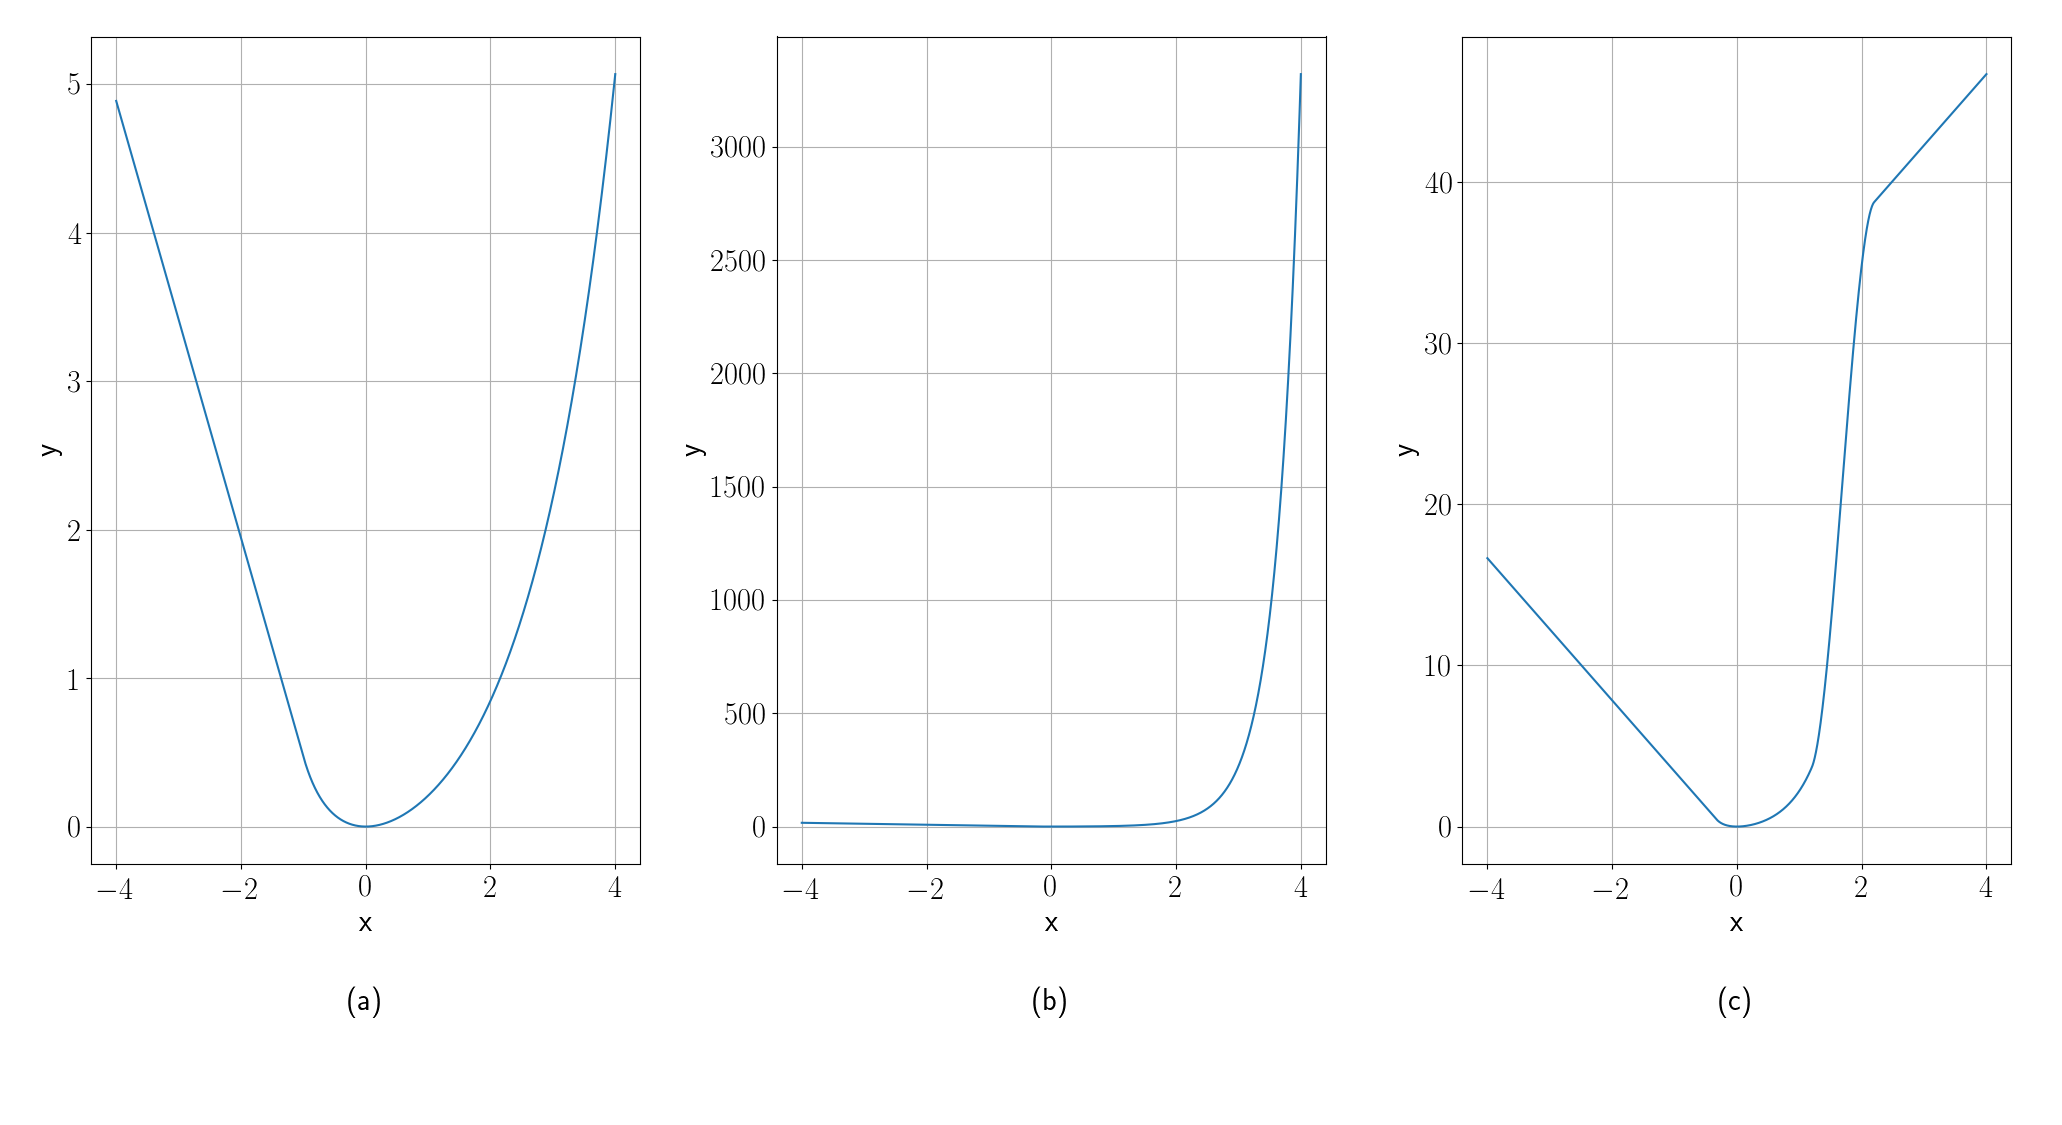
\includegraphics[width=\textwidth]{loss_evolution.png}
\caption[Loss iterations]{Three different stages of the custom loss function. (a): The loss as defined in \eqref{def:loss_original}. For $\left|x\right|<2$ the eyponential part is actually smaller than the linear part. This is not desirable, as for most of our testing the label for pure noise is about $4$ away from the smallest label for a signal. (b): To fix the issue of a too small exponential for some purposes, one can introduce a squish factor, that simply multiplies the input by some fixed value. In this case a squish factor of 3 was used. The values in general are a lot larger. (c): Having a large squish factor as in (b) introduces the problem of too large gradients. For this purpose, a cutoff can be introduced. This cutoff grows linearly with the same slope as the linear part of \eqref{def:loss_squished}. The transition between the exponential and linear part however needs to be of class $C^1$, so that the backpropagation algorithm can optimize. Therefore a spline polynomial connects the two parts.}\label{fig:loss_evolution}
\end{figure}
\clearpage

\section{Illustrations Final Architecture}\label{app:illustrations_final_architecture}
\begin{figure}[H]
\centering
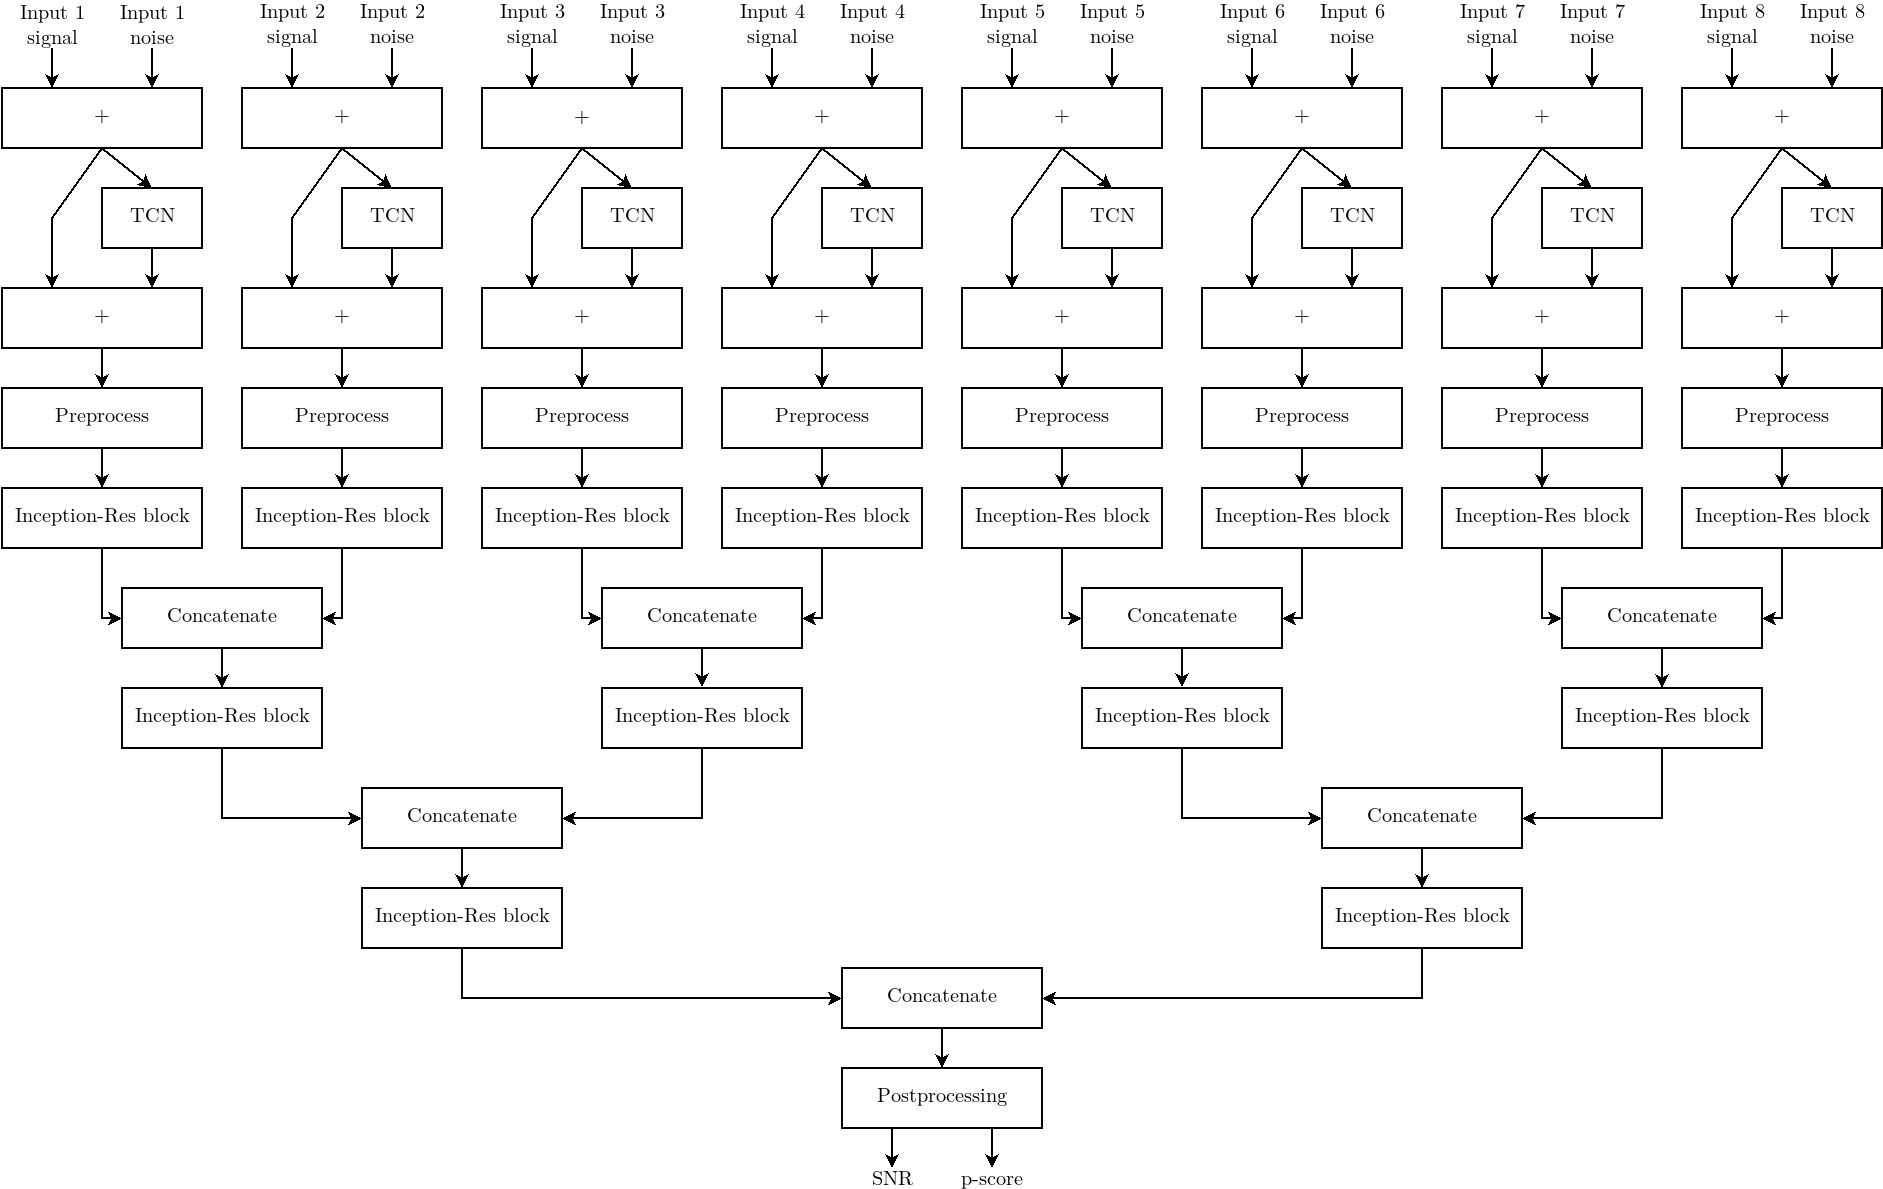
\includegraphics[angle=-90, origin=c, height=0.65\textheight]{Final_architecture.png}
\caption[Overview final architecture]{Shown is a high level overview of the final neural network architecture. The illustration does not show the auxilliary outputs after every \gls{tcn} and after all but the last concatenation layer. The first set of auxilliary ouputs are simply the outputs of the \gls{tcn} and trained for the pure waveform. The second set of auxilliary outputs takes the output of the concatenation layers and feeds them through an average pooling and a dimensional reduction layer, before condensing them down to a single number. This number is trained to be the \gls{snr} label. The reason or these auxilliary outputs is to combat the vanishing gradient problem.}\label{fig:high_level_final_network}
\end{figure}
\begin{figure}[h]
\centering
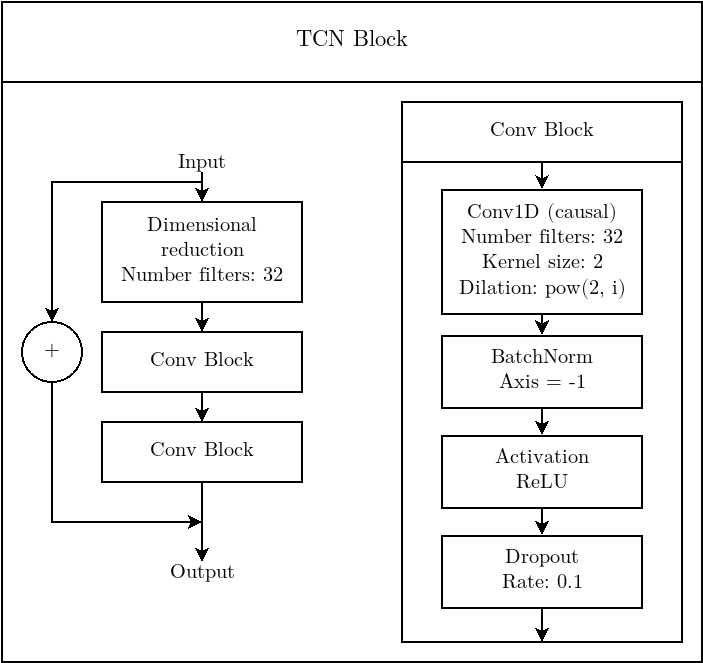
\includegraphics[width=0.5\textwidth]{TCN-block.png}
\caption[TCN-Block]{Shown is a single \gls{tcn}-block at depth $i$. A complete \gls{tcn} stacks multiple of these on top of each other.}\label{fig:tcn_block}
\end{figure}
\begin{figure}[h]
\centering
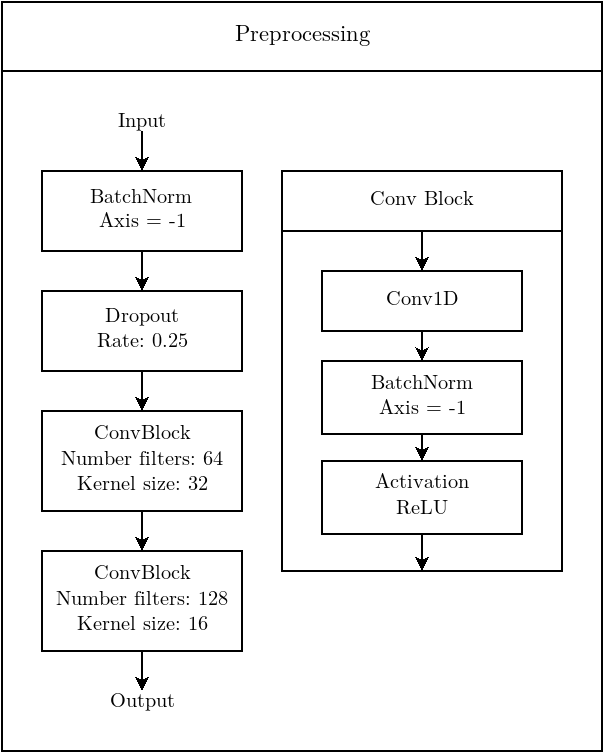
\includegraphics[width=0.5\textwidth]{Preprocessing.png}
\caption[Preprocessing of inception network]{Shown are the specific layers of the preprocessing step in the final network. A ConvBlock with a specified kernel size and number of  filters is understood to have a convolution layer with these properties.}\label{fig:preprocessing}
\end{figure}
\begin{figure}[h]
\centering
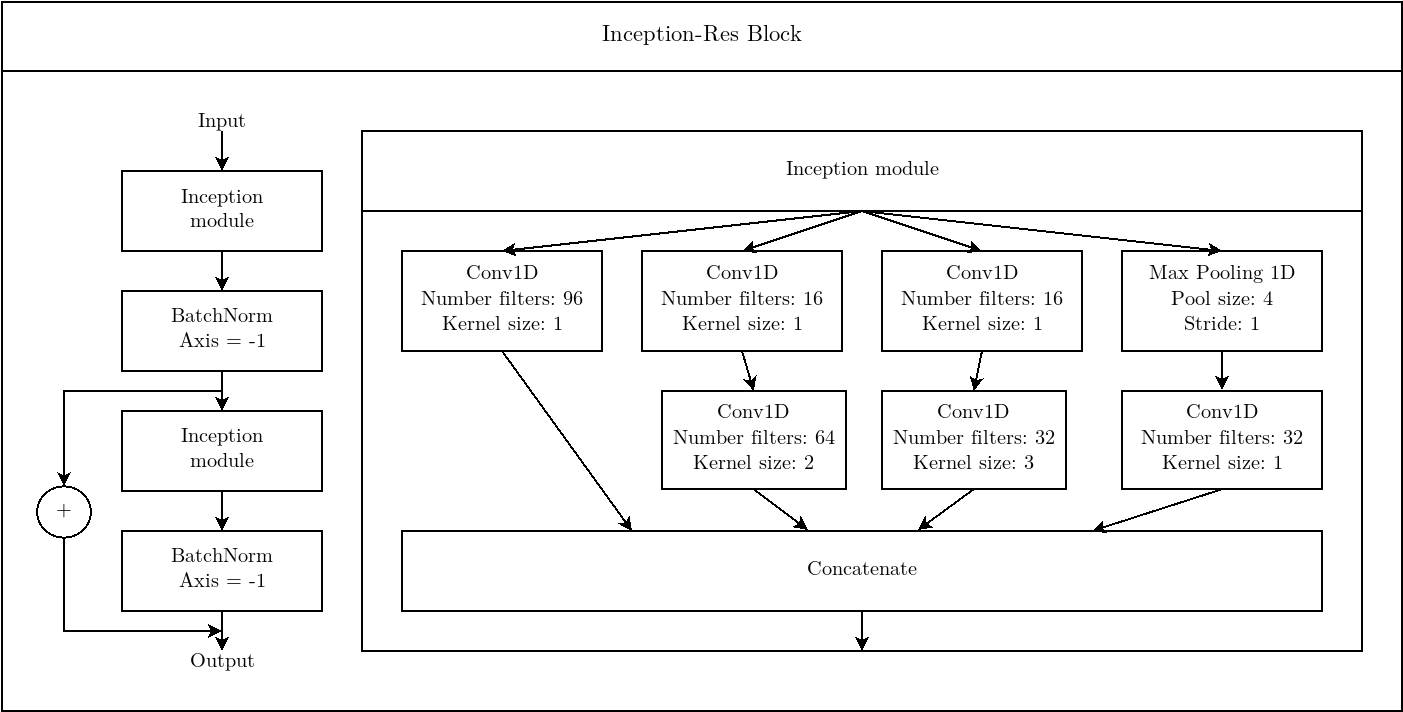
\includegraphics[width=\textwidth]{Inception_stack.png}
\caption[Inception-Res Block]{Shown is an inception block of the final architecture. Each one contains two inception modules, which are depicted to the right. Each layer of the inception module is equipped with a ReLU activation function and all convolution layers pad their input in such a way that the output has the same size as the input.}\label{fig:inception_block}
\end{figure}
\begin{figure}[h]
\centering
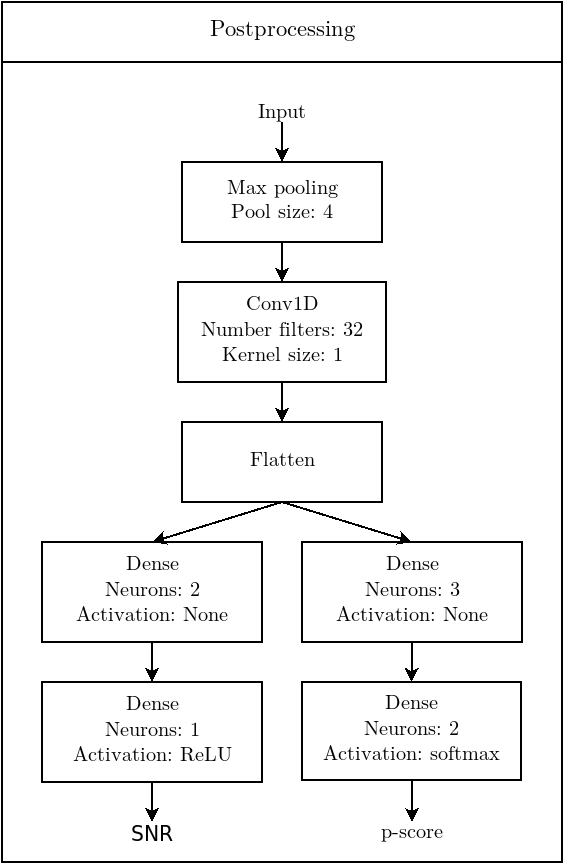
\includegraphics[height=0.5\textheight]{postprocessing.png}
\caption[Postprocessing of inception network]{Shown are the specific layers of the postprocessing step. They are mainly used to reduce the output of the collect-inception network that preceed it to the wanted quantities and their shapes.}\label{fig:postprocessing}
\end{figure}


\newpage
$\ $
\newpage

\printglossaries

\newpage
$\ $
\newpage
\printbibliography[heading=bibintoc]

\end{document}
